%%%%%%%%%%%%%%%%%%%%%%%%%%%%%%%%%%%%%%%%%
% Masters/Doctoral Thesis 
% LaTeX Template
% Version 2.5 (27/8/17)
%
% This template was downloaded from:
% http://www.LaTeXTemplates.com
%
% Version 2.x major modifications by:
% Vel (vel@latextemplates.com)
%
% This template is based on a template by:
% Steve Gunn (http://users.ecs.soton.ac.uk/srg/softwaretools/document/templates/)
% Sunil Patel (http://www.sunilpatel.co.uk/thesis-template/)
%
% Template license:
% CC BY-NC-SA 3.0 (http://creativecommons.org/licenses/by-nc-sa/3.0/)
%
%%%%%%%%%%%%%%%%%%%%%%%%%%%%%%%%%%%%%%%%%

%----------------------------------------------------------------------------------------
%	PACKAGES AND OTHER DOCUMENT CONFIGURATIONS
%----------------------------------------------------------------------------------------

\documentclass[
11pt, % The default document font size, options: 10pt, 11pt, 12pt
%oneside, % Two side (alternating margins) for binding by default, uncomment to switch to one side
english, % ngerman for German
singlespacing, % Single line spacing, alternatives: onehalfspacing or doublespacing
%draft, % Uncomment to enable draft mode (no pictures, no links, overfull hboxes indicated)
%nolistspacing, % If the document is onehalfspacing or doublespacing, uncomment this to set spacing in lists to single
%liststotoc, % Uncomment to add the list of figures/tables/etc to the table of contents
%toctotoc, % Uncomment to add the main table of contents to the table of contents
%parskip, % Uncomment to add space between paragraphs
%nohyperref, % Uncomment to not load the hyperref package
headsepline, % Uncomment to get a line under the header
%chapterinoneline, % Uncomment to place the chapter title next to the number on one line
%consistentlayout, % Uncomment to change the layout of the declaration, abstract and acknowledgements pages to match the default layout
]{MastersDoctoralThesis} % The class file specifying the document structure

%\usepackage[hyphens]{url}
\usepackage{setspace}
\usepackage{float}
\usepackage{subcaption}
%\usepackage{showframe}
\usepackage{microtype}
\usepackage{threeparttable}
\usepackage{graphicx}
\usepackage{adjustbox}
\usepackage[utf8]{inputenc} % Required for inputting international characters
\usepackage[T1]{fontenc} % Output font encoding for international characters
\usepackage{verbatim} % for comments
\usepackage{palatino} % Use the Palatino font by default

\usepackage[backend=bibtex,style=authoryear,natbib=true,doi=false,isbn=false,url=false]{biblatex} % Use the bibtex backend with the authoryear citation style (which resembles APA)

% \addbibresource{example.bib} % The filename of the bibliography
\addbibresource{references.bib} % mendeley

\usepackage[autostyle=true]{csquotes} % Required to generate language-dependent quotes in the bibliography

\usepackage[colorinlistoftodos,prependcaption,textsize=tiny]{todonotes}

% TODO disable hyphenation (for docx)
% \usepackage[none]{hyphenat}
% \usepackage[document]{ragged2e} 
% \raggedleft

%----------------------------------------------------------------------------------------
%	MARGIN SETTINGS
%----------------------------------------------------------------------------------------

\geometry{
	paper=a4paper, % Change to letterpaper for US letter
	inner=2.5cm, % Inner margin
	outer=3.8cm, % Outer margin
	bindingoffset=.5cm, % Binding offset
	top=1.5cm, % Top margin
	bottom=1.5cm, % Bottom margin
	%showframe, % Uncomment to show how the type block is set on the page
}

%----------------------------------------------------------------------------------------
%	THESIS INFORMATION
%----------------------------------------------------------------------------------------

\thesistitle{The Social AR Continuum:\\
Wearable AR for Sharing Social Experiences} % Your thesis title, this is used in the title and abstract, print it elsewhere with \ttitle
\supervisor{
Prof. Robert W. \textsc{Lindeman}\\
Prof. Mark \textsc{Billinghurst}\\
Dr. Gun \textsc{Lee}\\
Dr. Tobias \textsc{Langlotz}
} % Your supervisor's name, this is used in the title page, print it elsewhere with \supname

\examiner{} % Your examiner's name, this is not currently used anywhere in the template, print it elsewhere with \examname
\degree{Doctor of Philosophy} % Your degree name, this is used in the title page and abstract, print it elsewhere with \degreename
\author{Alaeddin \textsc{Nassani}} % Your name, this is used in the title page and abstract, print it elsewhere with \authorname
\addresses{} % Your address, this is not currently used anywhere in the template, print it elsewhere with \addressname

\subject{} % Your subject area, this is not currently used anywhere in the template, print it elsewhere with \subjectname
\keywords{} % Keywords for your thesis, this is not currently used anywhere in the template, print it elsewhere with \keywordnames
\university{\href{http://www.canterbury.ac.nz}{University of Canterbury}} % Your university's name and URL, this is used in the title page and abstract, print it elsewhere with \univname
\department{\href{http://hitlabnz.org/}{HIT Lab NZ}} % Your department's name and URL, this is used in the title page and abstract, print it elsewhere with \deptname
% \group{} % Your research group's name and URL, this is used in the title page, print it elsewhere with \groupname
\faculty{\href{http://www.canterbury.ac.nz/engineering/}{College of Engineering}} % Your faculty's name and URL, this is used in the title page and abstract, print it elsewhere with \facname

\AtBeginDocument{
\hypersetup{pdftitle=\ttitle} % Set the PDF's title to your title
\hypersetup{pdfauthor=\authorname} % Set the PDF's author to your name
\hypersetup{pdfkeywords=\keywordnames} % Set the PDF's keywords to your keywords
}

\begin{document}

\frontmatter % Use roman page numbering style (i, ii, iii, iv...) for the pre-content pages

\pagestyle{plain} % Default to the plain heading style until the thesis style is called for the body content

%----------------------------------------------------------------------------------------
%	TITLE PAGE
%----------------------------------------------------------------------------------------

\begin{titlepage}
\begin{center}

\vspace*{.06\textheight}
{\scshape\LARGE \univname\par}\vspace{1.5cm} % University name
\textsc{\Large Doctoral Thesis}\\[0.5cm] % Thesis type

\HRule \\[0.4cm] % Horizontal line
{\huge \bfseries \ttitle\par}\vspace{0.4cm} % Thesis title
\HRule \\[1.5cm] % Horizontal line
 
\begin{minipage}[t]{0.4\textwidth}
\begin{flushleft} \large
\emph{Author:}\\
{\authorname} % Author name - remove the \href bracket to remove the link
\end{flushleft}
\end{minipage}
\begin{minipage}[t]{0.4\textwidth}
\begin{flushright} \large
\emph{Supervisors:} \\
{\supname} % Supervisor name - remove the \href bracket to remove the link  
\end{flushright}
\end{minipage}\\[3cm]
 
\vfill

\large \textit{A thesis submitted in fulfilment of the requirements\\ for the degree of \degreename}\\[0.3cm] % University requirement text
\textit{in the}\\[0.4cm]
\deptname\\[2cm] % Research group name and department name
 
\vfill

{\large \today}\\[4cm] % Date
%\includegraphics{Logo} % University/department logo - uncomment to place it
 
\vfill
\end{center}
\end{titlepage}

% TODO: remove this 
\listoftodos

%----------------------------------------------------------------------------------------
%	DECLARATION PAGE
%----------------------------------------------------------------------------------------

\begin{declaration}
\addchaptertocentry{\authorshipname} % Add the declaration to the table of contents
\noindent I, \authorname, declare that this thesis titled, \enquote{\ttitle} and the work presented in it are my own. I confirm that:

\begin{itemize} 
\item This work was done wholly or mainly while in candidature for a research degree at this University.
\item Where any part of this thesis has previously been submitted for a degree or any other qualification at this University or any other institution, this has been clearly stated.
\item Where I have consulted the published work of others, this is always clearly attributed.
\item Where I have quoted from the work of others, the source is always given. With the exception of such quotations, this thesis is entirely my own work.
\item I have acknowledged all main sources of help.
\item Where the thesis is based on work done by myself jointly with others, I have made clear exactly what was done by others and what I have contributed myself.
\end{itemize}
 
\noindent Signed:\\
\rule[0.5em]{25em}{0.5pt} % This prints a line for the signature
 
\noindent Date:\\
\rule[0.5em]{25em}{0.5pt} % This prints a line to write the date
\end{declaration}

\cleardoublepage

%----------------------------------------------------------------------------------------
%	QUOTATION PAGE
%----------------------------------------------------------------------------------------

\vspace*{0.2\textheight}

\noindent\enquote{\itshape Thanks to my solid academic training, today I can write hundreds of words on virtually any topic without possessing a shred of information, which is how I got a good job in journalism.}\bigbreak

%----------------------------------------------------------------------------------------
%	ABSTRACT PAGE
%----------------------------------------------------------------------------------------

\begin{abstract}
\addchaptertocentry{\abstractname} % Add the abstract to the table of contents

The primary goal of the work reported in this thesis is to explore, develop and evaluate novel interaction techniques for Augmented Reality (AR) wearable headsets, focusing on how they can be used to share social experiences with family and friends. AR has the potential to provide an intuitive and natural approach to sharing our social experiences in life with others while being co-present. In order to better visualise and interact with social networks on wearable AR devices, we introduce the concept of the ``Social AR Continuum'', which describes the space of sharing experiences on AR in various dimensions. This work discusses the advantages and limitations of various implementations and techniques of shared social experiences on wearable AR.  

Based on Human-Computer Interaction methodologies, we conducted user studies to evaluate user presences and system usability of our implementation for visualising, sharing and interacting with social experiences on AR headsets. The work focused on the essential Social AR Continuum dimensions of representing contacts, sharing data and interactions, developed user interfaces on these dimensions and evaluated them using user studies. Our results show that using AR to share social experiences can increase users' social presence. The results are summarised as design recommendations to help interface designers better design shared social experiences on wearable AR systems. 

% Content: Can you insert in this where each of the user studies will be discussed? Also, don't you think the Social AR Continuum deserves its own chapter? Seems like one of the main topics of the thesis, and something you can attach your name to, so it should be highlighted. Also, there you can outline many possible axes, then go deep on the three you have chosen to explore. This indicates fertile areas that others can explore within the Continuum.

\end{abstract}


%----------------------------------------------------------------------------------------
%	ACKNOWLEDGEMENTS
%----------------------------------------------------------------------------------------

\begin{acknowledgements}
\addchaptertocentry{\acknowledgementname} % Add the acknowledgements to the table of contents
The acknowledgments and the people to thank go here, don't forget to include your project advisor\ldots
\end{acknowledgements}


%----------------------------------------------------------------------------------------
%	PREFACE
%----------------------------------------------------------------------------------------

\begin{preface}
\addchaptertocentry{\prefacename} % Add the preface to the table of contents

The research described in this dissertation has generated the following publications, which have appeared in the indicated peer-reviewed conference proceedings:

\noindent
\textbf{Chapter~\ref{ch:continuum} Social AR Continuum}
\begin{itemize}
    \item{ \fullcite{Nassani2017a}}
\end{itemize}

\noindent
\textbf{Chapter~\ref{ch:annotation} Annotation Continuum}
\begin{itemize}
    \item{ \fullcite{Nassani2016}}
    \item{ \fullcite{Nassani2015}}
    % \item{ \fullcite{Nassani2015a}}    
    \item{ \fullcite{Reichherzer2014}}
    % \item{ \fullcite{Billinghurst2014}}
\end{itemize}

\noindent
\textbf{Chapter~\ref{ch:data} Sharing Data Continuum}
\begin{itemize}
    \item{ \fullcite{Nassani2018a}}
    \item{ \fullcite{Nassani2018b}}
    \item{ \fullcite{Nassani2018c}}
\end{itemize}

\noindent
\textbf{Chapter~\ref{ch:contacts} Visualising Social Contacts}
\begin{itemize}
    \item{ \fullcite{Nassani2017b}}
    % \item{ \fullcite{Nassani2017}}
\end{itemize}

\end{preface}


%----------------------------------------------------------------------------------------
%	LIST OF CONTENTS/FIGURES/TABLES PAGES
%----------------------------------------------------------------------------------------
\setcounter{tocdepth}{1}
\tableofcontents % Prints the main table of contents

% \listoffigures % Prints the list of figures

% \listoftables % Prints the list of tables

%----------------------------------------------------------------------------------------
%	ABBREVIATIONS
%----------------------------------------------------------------------------------------

\begin{abbreviations}{ll} % Include a list of abbreviations (a table of two columns)

% \textbf{LAH} & \textbf{L}ist \textbf{A}bbreviations \textbf{H}ere\\
% \textbf{WSF} & \textbf{W}hat (it) \textbf{S}tands \textbf{F}or\\

\textbf{AR} & \textbf{A}ugmented \textbf{R}eality\\
\textbf{CCS} & \textbf{C}amera \textbf{C}oordinate \textbf{S}ystem\\
\textbf{DOF} & \textbf{D}egrees \textbf{O}f \textbf{F}reedom\\
\textbf{FPS} & \textbf{F}rames \textbf{P}er \textbf{S}econd\\
\textbf{HMD} & \textbf{H}ead \textbf{M}ounted \textbf{D}isplay\\
\textbf{HCI} & \textbf{H}uman-\textbf{C}omputer \textbf{I}nteraction\\
\textbf{UI} & \textbf{U}ser \textbf{I}nterface\\

\end{abbreviations}

%----------------------------------------------------------------------------------------
%	PHYSICAL CONSTANTS/OTHER DEFINITIONS
%----------------------------------------------------------------------------------------

% \begin{constants}{lr@{${}={}$}l} % The list of physical constants is a three column table

% % The \SI{}{} command is provided by the siunitx package, see its documentation for instructions on how to use it

% Speed of Light & $c_{0}$ & \SI{2.99792458e8}{\meter\per\second} (exact)\\
% %Constant Name & $Symbol$ & $Constant Value$ with units\\

% \end{constants}

%----------------------------------------------------------------------------------------
%	SYMBOLS
%----------------------------------------------------------------------------------------

% \begin{symbols}{lll} % Include a list of Symbols (a three column table)

% $a$ & distance & \si{\meter} \\
% $P$ & power & \si{\watt} (\si{\joule\per\second}) \\
% %Symbol & Name & Unit \\

% \addlinespace % Gap to separate the Roman symbols from the Greek

% $\omega$ & angular frequency & \si{\radian} \\

% \end{symbols}

%----------------------------------------------------------------------------------------
%	DEDICATION
%----------------------------------------------------------------------------------------

\dedicatory{For/Dedicated to/To my\ldots} 

%----------------------------------------------------------------------------------------
%	THESIS CONTENT - CHAPTERS
%----------------------------------------------------------------------------------------

\mainmatter % Begin numeric (1,2,3...) page numbering

\pagestyle{thesis} % Return the page headers back to the "thesis" style
\setstretch{1.5} 

% Include the chapters of the thesis as separate files from the Chapters folder
% Uncomment the lines as you write the chapters

\chapter{Introduction} % Main chapter title
\label{ch:intro} % Change X to a consecutive number; for referencing this chapter elsewhere, use \ref{ChapterX}

% In this chapter, we introduce mixed-reality continuum. AR/VR becoming popular. Previous research focus on single users or collaboration with few users. The question remain how AR will be used with many uses and in social situations. The Social AR Continuum can be an answer to this question.

Augmented Reality (AR) is technology that enables the seamless overlay of virtual images on the real world, so that both real and virtual can be seen and interacted with at the same time. 

\cite{azuma1997survey} defined AR as the coexistence of the virtual world and the real world "it would appear to the user that the virtual and real objects coexisted in the same space" (Figure \ref{fig:video-see-through}).

\begin{figure}
    \centering
    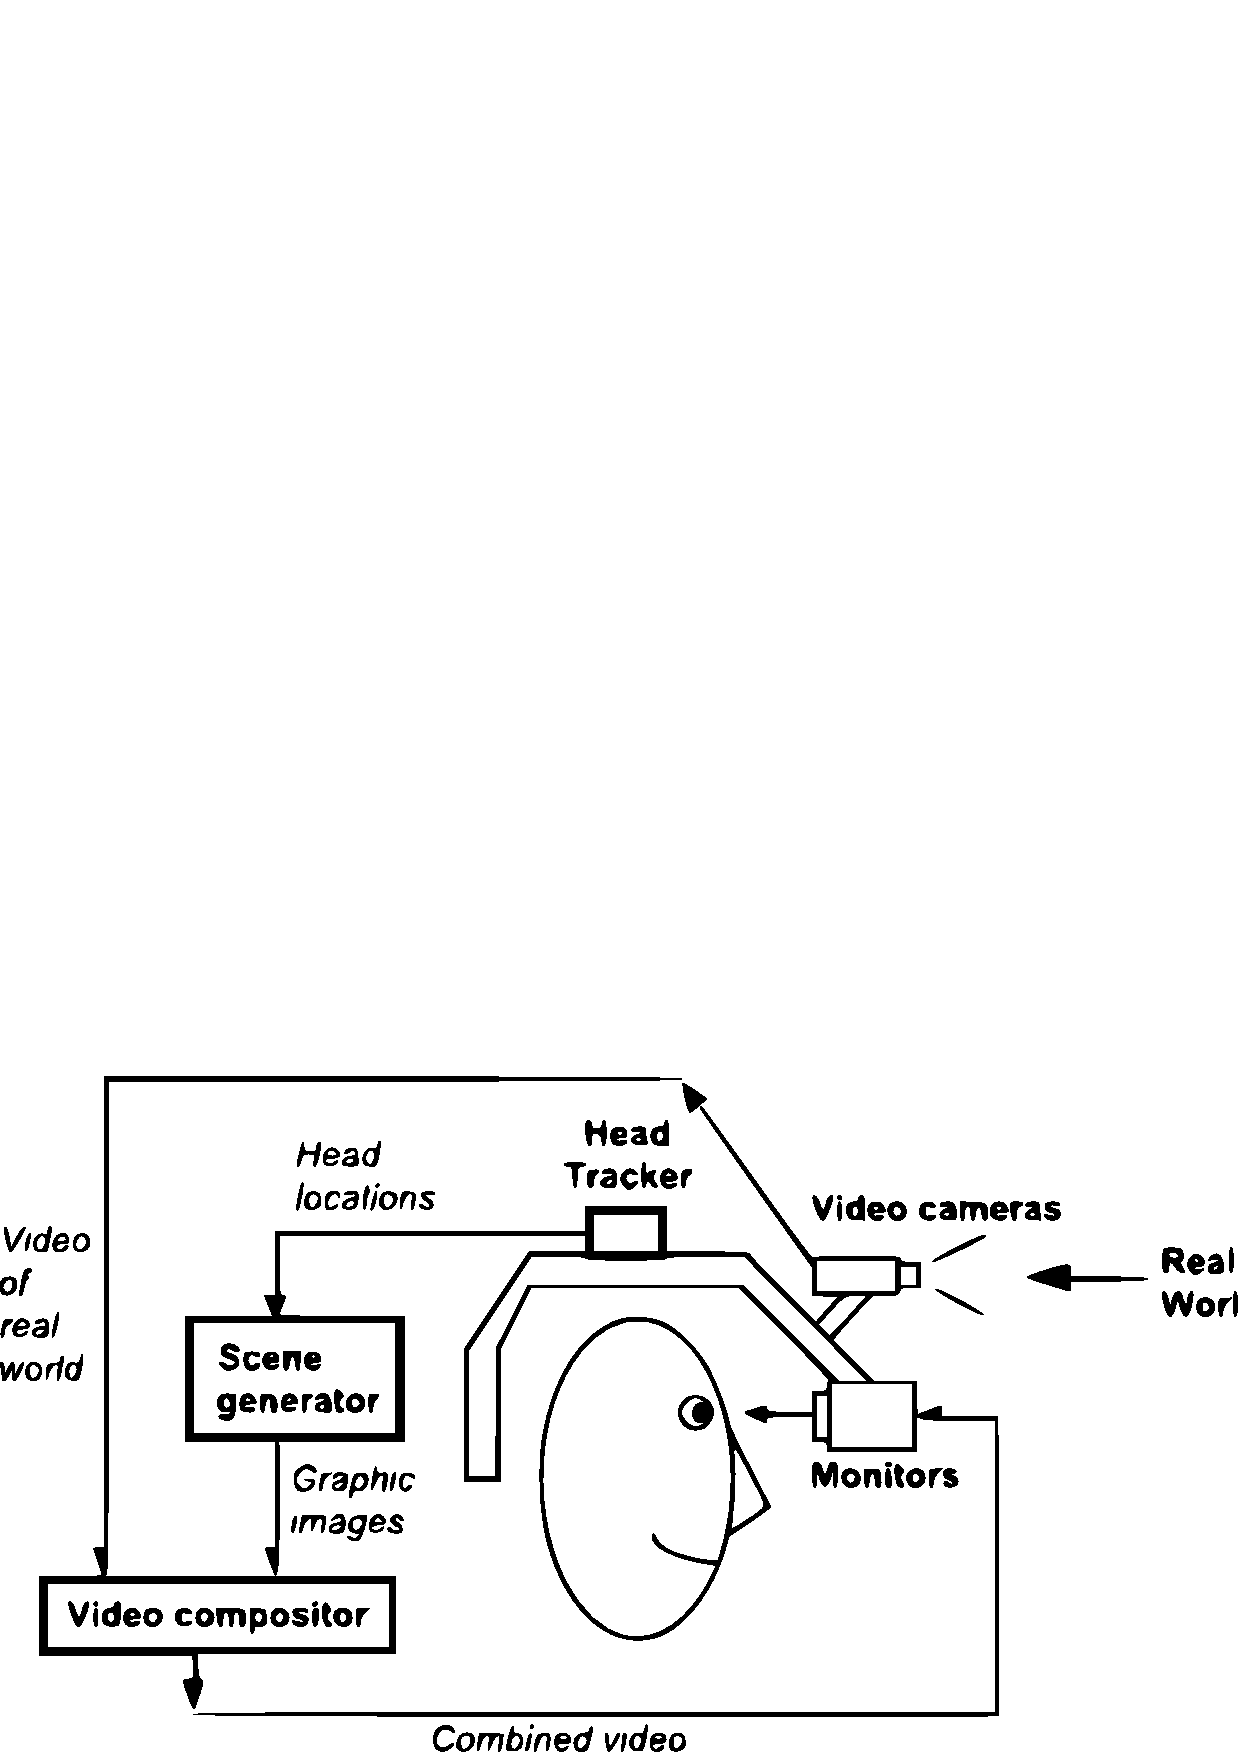
\includegraphics[width=.8\linewidth]{images/video-see-through-ar.png}
    \caption{video see-through AR display}
    \label{fig:video-see-through}
\end{figure}

Milgram \cite{Milgram1995a} defined the mixed reality (MR) continuum and placed augmented reality (mostly real content overlaid by virtual content) between virtual reality (VR) where full immersion of virtual contents and augmented virtuality (AV) where mostly virtual content overlaid by real content (Figure \ref{fig:mr-continuum}). 

\begin{figure}
    \centering
    \includegraphics[width=.8\linewidth]{images/mixed-reality-continuum.png}
    \caption{Mixed reality continuum}
    \label{fig:mr-continuum}
\end{figure}

\cite{Zhou2008, Kim2018} looked at trend of augmented reality in the academic conference ISMAR and looked at trends in research community and reported "dramatic increase of commercial interest in AR/MR" and "AR technology will continue to develop even more dynamically and effectively over the next ten years, toward the vision of pervasive presence in our daily lives.". AR display are getting more affordable with better rendering and registration techniques. Also AR displays are getting unteathered enabling mobile AR applications and self-contained displays are entering the market.

\section{Problem Statement}

This PhD thesis addresses the problems of: 
(1) using visualising and interacting with social contacts through wearable augmented reality displays. 
(2) displaying huge amount of 3D content of sharing social data that is overlaid over a limited available physical space through wearable AR devices. 
(3) defining and exploring the best ways to use wearable AR devices to connect with social networks.
The focus of this thesis is on enabling the use of wearable AR for sharing social experiences. 

% - The potential for AR to be a social sharing platform. \\
% - Sharing social experiences was not fully addressed in the research community

With major industry players (e.g. Microsoft, Facebook and Apple) supporting Augmented Reality (AR), more potential use of AR/VR could be for connecting with social networks. Just as people today use their mobile phones to connect with hundreds or thousands of "friends", wearable AR displays could be used to connect with friends and view and interact with their shared information.

Applications for Social VR and 360 video have been introduced on new VR headsets. For instance Facebook Spaces\footnote{https://www.facebook.com/spaces} allows VR users to connect with friends and family and share 360 photos and take selfies. AltSpaceVR\footnote{https://altvr.com/} was acquired by Microsoft and enable more diverse hand-held and wearable devices to be used for social connection with others. Most recently Magic Leap's Avatar Chat\footnote{https://www.magicleap.com/stories/blog/connect-with-friends-with-avatar-chat} offers similar experences where avatars representing social friends are displayed in an AR space. 

Previously, handheld AR systems have been used to view social networks in a number of different ways. For example, Presslite's Twitter 360\footnote{https://www.youtube.com/watch?v=5w7EAz8-uwU} shows virtual tweets overlaid on the real world at the locations of the people that sent them (see figure \ref{fig:presslite}), and early versions of Junaio\footnote{https://en.wikipedia.org/wiki/Junaio} allowed people to drop virtual messages and pictures in the real world, as did the popular application Sekai Camera\footnote{https://www.youtube.com/watch?v=oxnKOQkWwF8}. Most of these applications were focused on asynchronous collaboration, enabling people to post virtual messages in space which can later be browsed and retrieved by other users. 

\begin{figure}
    \centering
    \includegraphics[width=.8\linewidth]{images/Presslite-twitter-360.PNG}
    \caption{Presslite's Twitter 360 AR interface}
    \label{fig:presslite}
\end{figure}

However similar technology could also be used for live synchronous collaboration such as live video avatar sharing  \cite{Billinghurst2002}, or sharing realistic 3D models superimposed over the real world \cite{Fanello2016}, or by using virtual avatars to show a live view of remote collaborators and their surrounding space as in the Holoportation system \cite{Fanello2016} (see figure \ref{fig:holoportation}).

\cite{Peddie2017} reviewed the historic uses of wearable displays and AR displays. 

\begin{figure}
    \centering
    \includegraphics[width=.8\linewidth]{images/holoportation.png}
    \caption{Holoportation}
    \label{fig:holoportation}
\end{figure}

% Tobias: Make clear here that scrolling etc is no option as we are constrained by the interactions and would require unobtrusive interactions.
By using a wearable AR display like the Microsoft HoloLens\footnote{https://www.microsoft.com/en-nz/hololens}, it could be possible for user to see an AR representation of their social network visible at all times. However, this raise the question of how to visually represent the user's contacts in the network. For example, if a user has a large social network with hundreds of contacts available, visually representing each of themmight clutter the user's visual space.

% This research focus on how to represent a social network with hundreds or thousands of contacts in a wearable AR interface. For example, if there are dozens of virtual tags in an AR view representing people, how can user be able to distinguish between each one? How will this interface scale to support hundreds or thousands of people? This is an important area of research as it will allow users to view and interact with a large number of social network followers in a wearable AR systems, at different levels of privacy and social engagement.

% One of the challenges we are seeking to address is how to manage and represent communication from dozens, hundreds or thousands of contacts in a social network in an AR interface. If there are dozens of virtual tags in view representing people on the user's social network, how can they be distinguished between each other? How will the AR interface scale to hundreds or thousands of people?

\section{Research Questions}

This thesis targets the future where AR devices are used everyday, and social networks are visualised in the AR view. So we address the following research questions: 

\begin{itemize}
    % (chapter 3 - Social AR continuum)
    \item RQ1: How to represent social networks and shared social data on wearable AR devices 
    
    \item RQ1(option 2): What dimensions/factors/parameters in sharing social experiences on wearable AR devices 
    
    % (chapter 4 - annotation continuum)
    \item RQ2: How to represent annotations/tags on shared social experience through wearable AR devices
    
    % (chapter 5 - Sharing data continuum)
    \item RQ3: How to share virtual objects/data with our social network through wearable AR 
    
    % (chapter 6 - visualising social contacts) 
    \item RQ4: How to visualise our social contacts as virtual avatars through wearable AR devices

\end{itemize}

To answer the research questions, this thesis explores how wearable AR can be used for sharing social experiences. These explorations identifies the parameters at which AR sharing for social reasons happen. Once the parameters are defined, we build few system prototypes as a proof of concept of the experience or the interaction design. We then run user studies to test the objectives of the system with human participants. We observe their behaviour and report on the results of these experiments. 

\section{Contributions}

1) Definition of parameters and dimensions of the social AR continuum 
This thesis' main contribution is defining the social AR continuum space which consists of set of parameters that define the space of sharing social experience through AR wearable/hand-held devices. We define the space of AR continuum by exploring the main parameters that can be varied based on the social proximity. These parameters are grouped into the following categories 1) self and other, 2) shared objects and annotation and 3) surrounding environments. Under each of these categories we define the dimensions of variables that affect the shared social experience. 

2) The implementation of the AR experience user interface. For each dimension defined on the continuum, we built a software and hardware prototype to test the user interface design with human subjects. The implementation details are described in the thesis for future studies purposes.

3) User studies and evaluation to validate the parameters of the social AR continuum.  we built a prototype and run a user-study/focus-group to validate the dimensions on the social AR continuum. 

3) High-level design guidelines for interface designers who are building social sharing experiences on AR devices. One of the outcomes of defining the social AR continuum and validating these dimnesions is that it can serve as a high-level experience design guidelines that helps individual/organisations to create AR experiences for social sharing and connection purposes.


% This research is novel and makes the following contributions:

% \begin{itemize}
%     \item Defining the dimensions in design space of sharing social experiences on wearable AR
%     \item Technical implementing different prototypes of sharing social experiences on wearable devices
%     \item User study evaluations of behaviour and preception of using social AR prototypes.
% \end{itemize}


In summary, this thesis helps to increase the understanding on how to share social experiences through AR devices. The results of the user experiements conducted throughout this research help identifying the imapact of the the social AR continuum parameters on presence, user engagement and user interface usablity, which serves as a guideline for future designs. 

The rest of the thesis is organised as follows: Chapter \ref{ch:continuum} describes the social AR continuum and the parameters/ dimensions involved. Chapter \ref{ch:annotation} describes the shared data and annotation continuum including different implementation of shared annotation and awareness cues on different platforms (handheld and wearable). Chapter \ref{ch:data} describes the surrounding environment continuum including shared 360 videos and 30 captured spaces. Chapter \ref{ch:contacts} describes the continuum of self and others of representing social contacts networks on AR devices. 

\section{Selected Publications}

The main results of this thesis have appeared in a number of peer reviewed publications from scientific conferences in AR and HCI, including: 

\begin{itemize}
    \item{ \fullcite{Nassani2017a}}
    \item{ \fullcite{Nassani2016}}
    \item{ \fullcite{Nassani2015}}
    \item{ \fullcite{Nassani2015a}}    
    \item{ \fullcite{Reichherzer2014}}
    \item{ \fullcite{Billinghurst2014}}
    \item{ \fullcite{Nassani2018a}}
    \item{ \fullcite{Nassani2018b}}
    \item{ \fullcite{Nassani2018c}}
    \item{ \fullcite{Nassani2017b}}
    \item{ \fullcite{Nassani2017}}
\end{itemize}

The above publications help answering the research questions of thesis including how to share social experiences on AR devices for each category on the social AR continuum. 

% \todo[inline]{Mark: In the remainder of the thesis we first review related work and explain the research gap that our work files (section 2). Then [put  more here – summarise the thesis structure] }

% \todo[inline]{[You may also want to put together a  thesis outline chart. Basically showing the experiments you conducted and  prototypes you developed and  how these  contribute to addressing  the research questions that you’ve raised. This is helpful if you have a lot of material to report on, so the reviewers can understand how it all fits together] }

\chapter{Related Work} % Main chapter title

\label{ch:background} % Change X to a consecutive number; for referencing this chapter elsewhere, use \ref{ChapterX}
This work extends earlier work in wearable AR, AR annotation, social proximity, virtual avatars, research collaboration, telepresence and sharing social experiences. This section examines previous related work on wearable AR, AR collaboration, and sharing social experiences from the social AR perspective. 

\section{Wearable AR} 

AR devices can be categorised into wearable (e.g., head-mounted displays, helmet or contact lens), handheld (e.g., phone, tablet) or projected displays where AR is projected onto a larger area regardless of where the user is looking~\cite{Peddie2017}. 

\cite{Feiner1997a} presented the first mobile wearable AR system in 1997 called "Touring Machine" combining a head-mounted display (HMD), hand-held tablet, and a backpack carrying a computer GPS and radio for wireless access. \cite{Hollerer1999} followed up and explored different user interfaces on a wearable see-through display. The interface allowed users to sketch pathways and annotate their world for collaborative AR systems. 

Wearable AR has added an extra dimension to AR allowing people to collaborate hands-free. \cite{Feiner1999} talked about what impact wearable computing (and being mobile in general) has from the social perspective. These implications include personal privacy concerns, connectivity, collaboration and how it looks and feels. 

Wearable AR has been explored for social interactions. For instance, \cite{Cheok2002a} developed a wearable mixed reality experience where social interactions take place. \cite{Amores2015} used gestures to communicate social interactions via wearable devices. \cite{Lee2019} used live 360 cameras to communicate between worker and helper. \cite{Shu2018} developed a system of facial recognition to facilitate social interactions. 

With wearable AR devices becoming affordable, available and ubiquitous, there is a need to understand design considerations for this new platform. Previous research has looked into using AR headsets for collaborative use. For example in enhancing face to face \cite{Billinghurst2002} or remote collaboration \cite{Gupta2016}. The research presented here explores the use of AR headsets for social interaction and shared experiences. Social interactions can be extrapolated from current social network interactions where \enquote{friends} share content and interact with another's content (i.e., placing likes and comments).

% There is a need to understand design considerations for this new platform. Previous research has looked into using wearable AR headsets for collaborative use, for example in enhancing face to face \cite{Billinghurst2002} or remote collaboration \cite{gupta2016you}. The research presented here explores the use of AR headsets for social interaction and shared experiences. 

\section{AR Annotation, Collaboration and Telepresence}

There are a number of examples of AR annotation demonstrations on mobile devices. For example, mobile AR browsers (e.g., Wikitude\footnote{https://www.wikitude.com/} or Junaio\footnote{https://en.wikipedia.org/wiki/Junaio}) can overlay AR tags in the real world using GPS and other motions sensors. While they were successful in demonstrating the concept of visualising AR annotation, the registration of virtual objects in the real world can be inaccurate and they can only be used in outdoor, large-scale environments. Mobile AR browsers usually create AR tags in advance, but recent research projects have investigated in-situ and interactive creation of AR tags. For example, \cite{Kim:2011:IAS} presented an interactive method where the user stands in a fixed position to calibrate the room model with the gyroscope data. The user can then touch and annotate locations with a rectangle where virtual content, like text, images and 3D models, can be overlaid. \cite{Langlotz:2012:OCP} developed a vision-based orientation tracking system to locate and visualise annotations with pixel accuracy on a real-time generated panorama. These systems assume pure rotation from the devices while the user has to stand at the same position while doing the annotation, which dramatically degrades the quality of the user experience.

A variety of AR annotation methods with wearable interfaces have also been presented. Sixsense \cite{Mistry:2009:WWU} used a wearable gestural interface for AR annotation. It consists of a camera and a small projector mounted on a hat or in a pendant. The camera tracks user hand gestures and the projector visually augments virtual content onto the physical objects with which the user is interacting. However, the system requires planar surfaces in front of the user for accurate projection because of the lack of a depth sensor. OmniTouch \cite{Harrison:2011:OTW} is a wearable projection system equipped with depth-sensing technology that enables interactive multi-touch applications on different surfaces. Both the depth camera and projector are mounted onto a form-fitting metal frame, which is worn on the shoulders, and secured with a chest strap. This system extends the typical scenarios supported by Sixsense to on-body surfaces or objects held in the hand for image projection. However, the system was still bulky and inconvenient to use because it needed to be connected to a desktop computer.

\begin{figure}
    \centering
    \includegraphics[width=\linewidth]{images/Huang2013.PNG}
    \caption{HandsInAir: A Wearable System for Remote Collaboration}
    \label{fig:HandsInAir}
\end{figure}

Camera-equipped mobile devices provide a quick way of capturing and sharing experiences and spaces. Wearable computers that combine HMDs and cameras provide new opportunities for collaboration. For example, the Google Glass\footnote{http://www.google.com/glass/} wearable system has a camera, mic, and head-worn display.

There has been a significant amount of earlier research on remote collaboration using head-mounted cameras and displays. For example, allowing a remote user to place virtual annotations on the live camera view from a head-worn camera and showing the result in the wearers HMD, has been shown to enhance remote collaboration \cite{Fussell2003}. Other systems allow a remote user to place their hands in the local user's view \cite{Huang2013} (Figure \ref{fig:HandsInAir}). 

In many wearable and mobile AR applications, remote collaboration is the main purpose for sharing a view of the user's world. For example, remote expert collaboration systems have been developed where a local worker with an AR display can share a live video view of their workspace with a remote expert \cite{Billinghurst2002}. The remote expert can provide visual feedback with AR graphical cues.  However, most of these systems have just been developed for collaboration between small numbers of users, and not for more extensive social networks. (Figure \ref{fig:Billinghurst2002})

\begin{figure}
    \centering
    \includegraphics[width=\linewidth]{images/Billinghurst2002.PNG}
    \caption{Live virtual video avatars for remote collaborative AR interfaces. \cite{Billinghurst2002}}
    \label{fig:Billinghurst2002}
\end{figure}

When people connect in this way, they may also want to share different amounts of information about their surroundings with each other. For example, users who are close friends in a social network may be happy to share a 3D virtual view of their surroundings and have the remote user appear as an AR avatar in their real space, while those that are strangers may only want to have an audio connection and not show anything of their surroundings to preserve their privacy \cite{Oetzel2011}. The position on the social continuum could be used to modify how much information a person can share about themselves and their surroundings.

\cite{Fuchs2014} (Figure \ref{fig:Fuchs2014}) studied telepresence via a scanned 3D environment to enable social connections with people and simulated face-to-face interactions. The remote person was scanned and reconstructed live in the local environment. They forecasted that 3D telepresence was going to be more popular when technology becomes more capable.

\begin{figure}
    \centering
    \includegraphics[width=.8\linewidth]{images/Fuchs2014.PNG}
    \caption{Real-time 3D reconstruction of human \cite{Fuchs2014}}
    \label{fig:Fuchs2014}
\end{figure}

\section{Social Proximity \& Virtual Avatars}

In the social AR/VR space, previous work implemented a variety of visual representations of self and others. \cite{Fanello2016} prototyped live sharing of a full scan of a person's body with remote users using 3D cameras and the HoloLens\footnote{https://www.microsoft.com/en-nz/hololens}. For representing “people” in AR space, \cite{Sousa2016} (Figure \ref{fig:Sousa2016}) studied the concept of \enquote{personal space} and \enquote{social bubbles} in terms of proxemic interactions between people in different places. They used floor projections and hand-held devices to communicate the presence of remote people. They also established a \enquote{gradual engagement model for remote proxemics} based on distance from the user which consisted of 1) personal, 2) engaged, 3) peripheral and 4) ambient.

\begin{figure}
    \centering
    \includegraphics[width=.8\linewidth]{images/Sousa2016.PNG}
    \caption{Gradual engagement model for remote proxemics. \cite{Sousa2016}}
    \label{fig:Sousa2016}
\end{figure}

Most previous work has focused on how visual representation and proximity could be used to organise an AR representation of a person's social network. However, this information could also be used to modify the contextual information being shared by a user out to their social network as well. 
% For example, a person may not want strangers to know what they look like, and so would prefer being represented as a stylistic icon to people that do not know them, but would be more comfortable sharing a lifelike representation to those that are close to them. 

Similarly, some companies (such as High Fidelity\footnote{https://highfidelity.com/}, Sansar\footnote{https://www.sansar.com/}, Itsme3D\footnote{https://www.itsme3d.com/}) and other VR shared worlds) are building social VR experiences in which users are represented as 3D virtual avatars. In the social VR space, previous work implemented a variety of visual representations of self and others. For instance, virtual avatars have been used to share social experiences such as in Facebook Spaces\footnote{https://www.facebook.com/spaces} (Figure \ref{fig:facebook-spaces}, left) where users can meet in VR, take selfies and teleport to a 360-degree video. Virtual avatars for self and others are represented as floating face and upper body rendered in a VR background. 

\begin{figure}
    \centering
    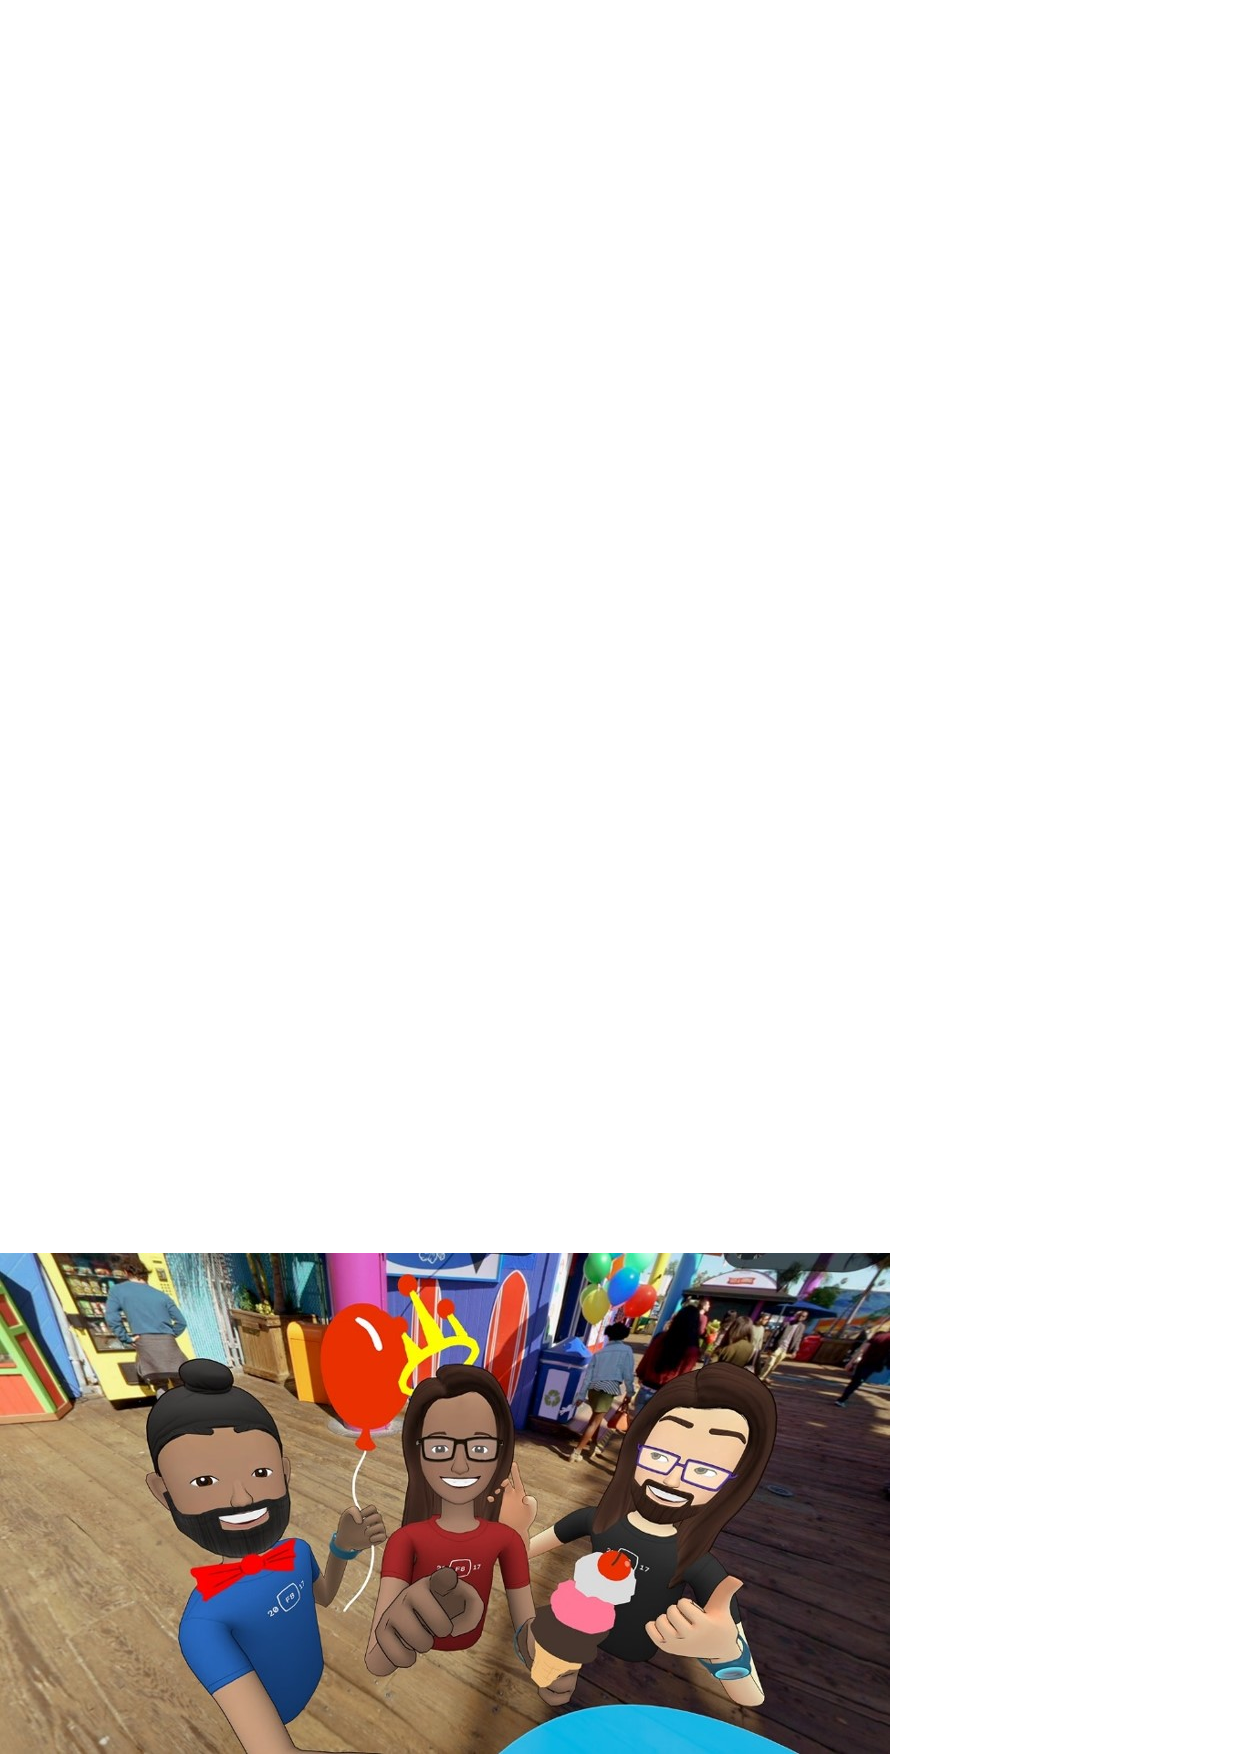
\includegraphics[width=.4\linewidth]{images/facebook-spaces.jpg}
    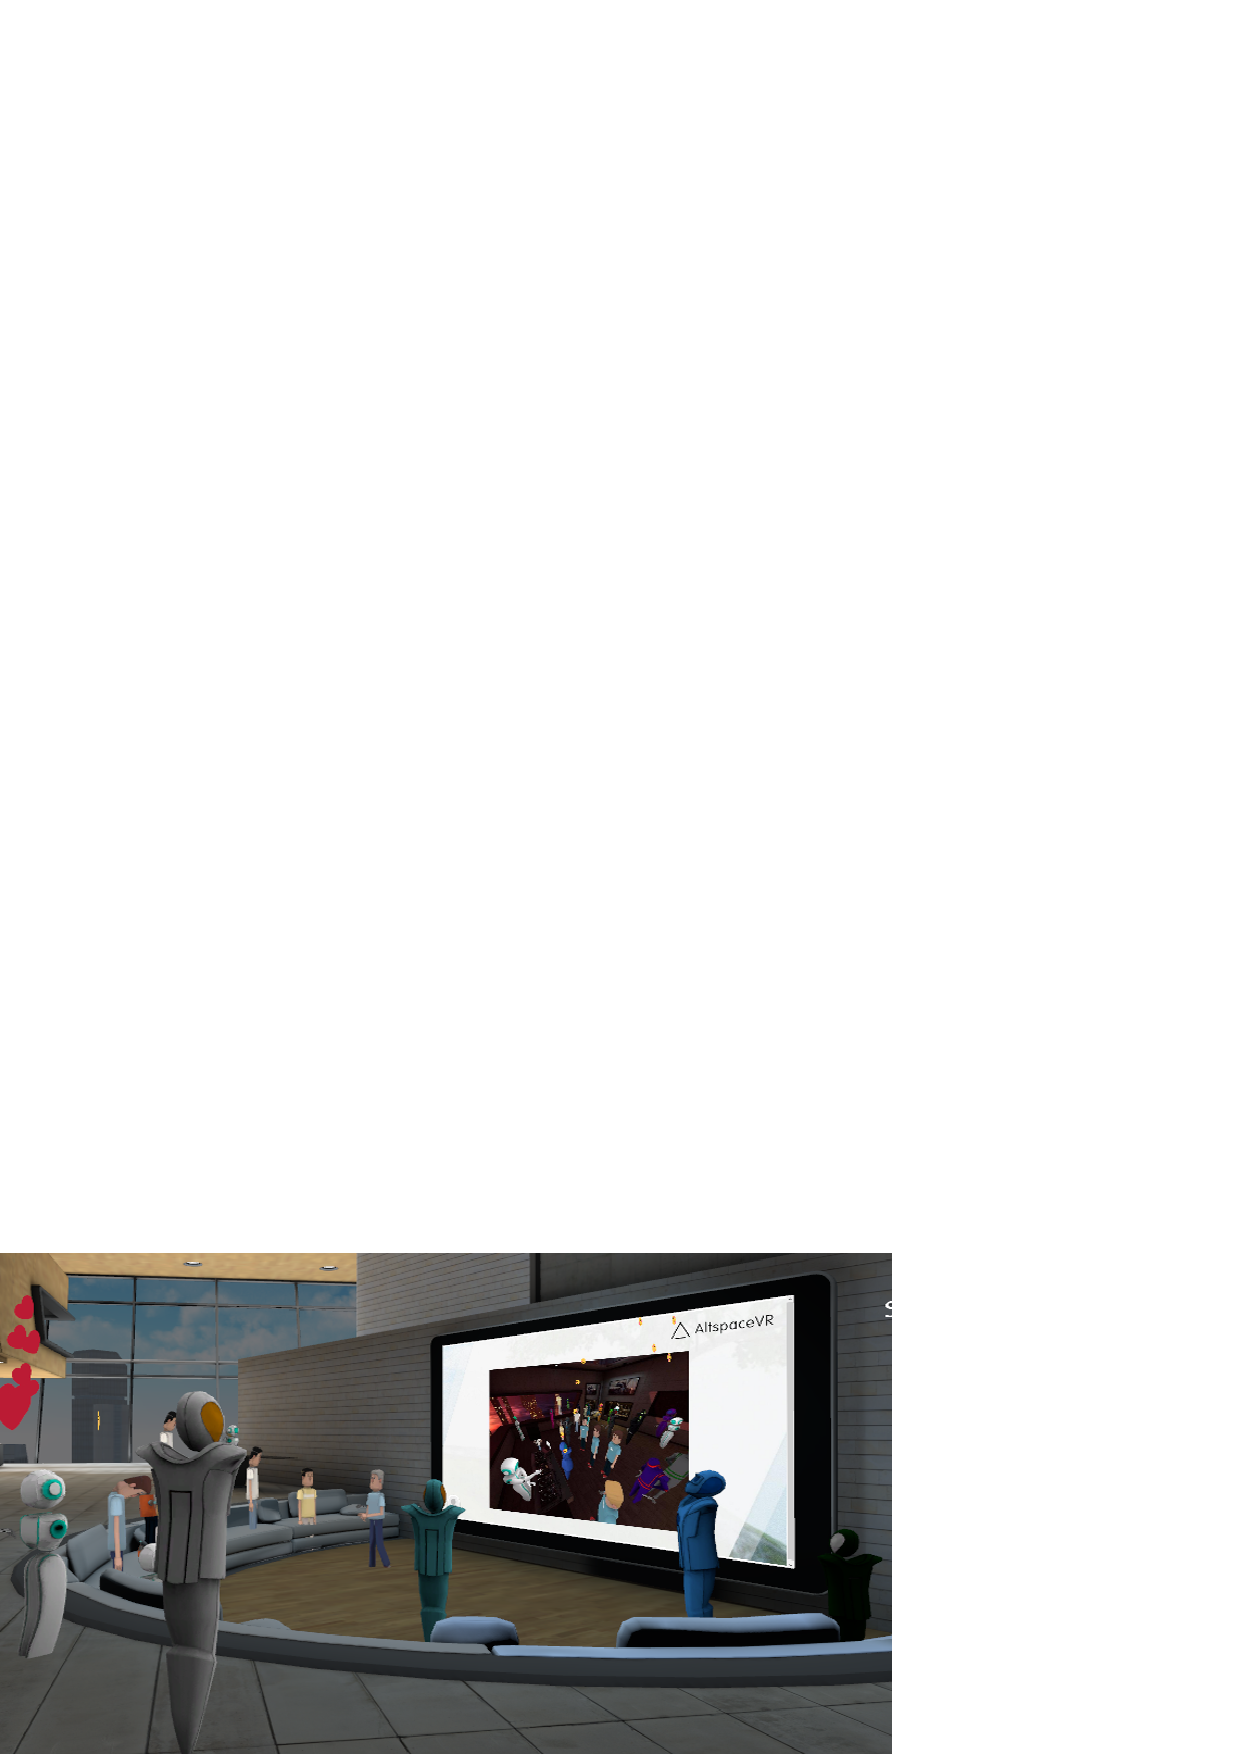
\includegraphics[width=.4\linewidth]{images/altspace-vr.png}
    \caption{Examples of avatars in VR. Facebook Spaces (left) and AltSpaceVR (right)}
    \label{fig:facebook-spaces}
\end{figure}

As for the social AR spaces, there have been limited examples of social applications. Avatar Chat was introduced by Magic Leap\footnote{https://www.magicleap.com/experiences/social} (Figure \ref{fig:ml-avatar-chat}) in late 2018. The app allows users to connect with their social contacts and view their avatar overlaid on top of their physical environment. Users can share emojis, connect to a group "avatar" chat and talk about images overlaid in their space. The avatars are cartoonish-looking representing the upper half of the body floating in the AR space. Natural hand gestures are detected using the depth cameras on the device, assisted by computer vision algorithms and translated to a pre-defined set of virtual hand gestures to the other participants in the chat session. 

Saptiate\footnote{http://spatiate.com/} is another social app launched in early 2019 on Magic Leap where users can connect in a chat session with primitive avatars, sketch in their AR world, and share the sketching in real time with connected users. The users can see each other's avatars and hear their voices. 

\begin{figure}
    \centering
    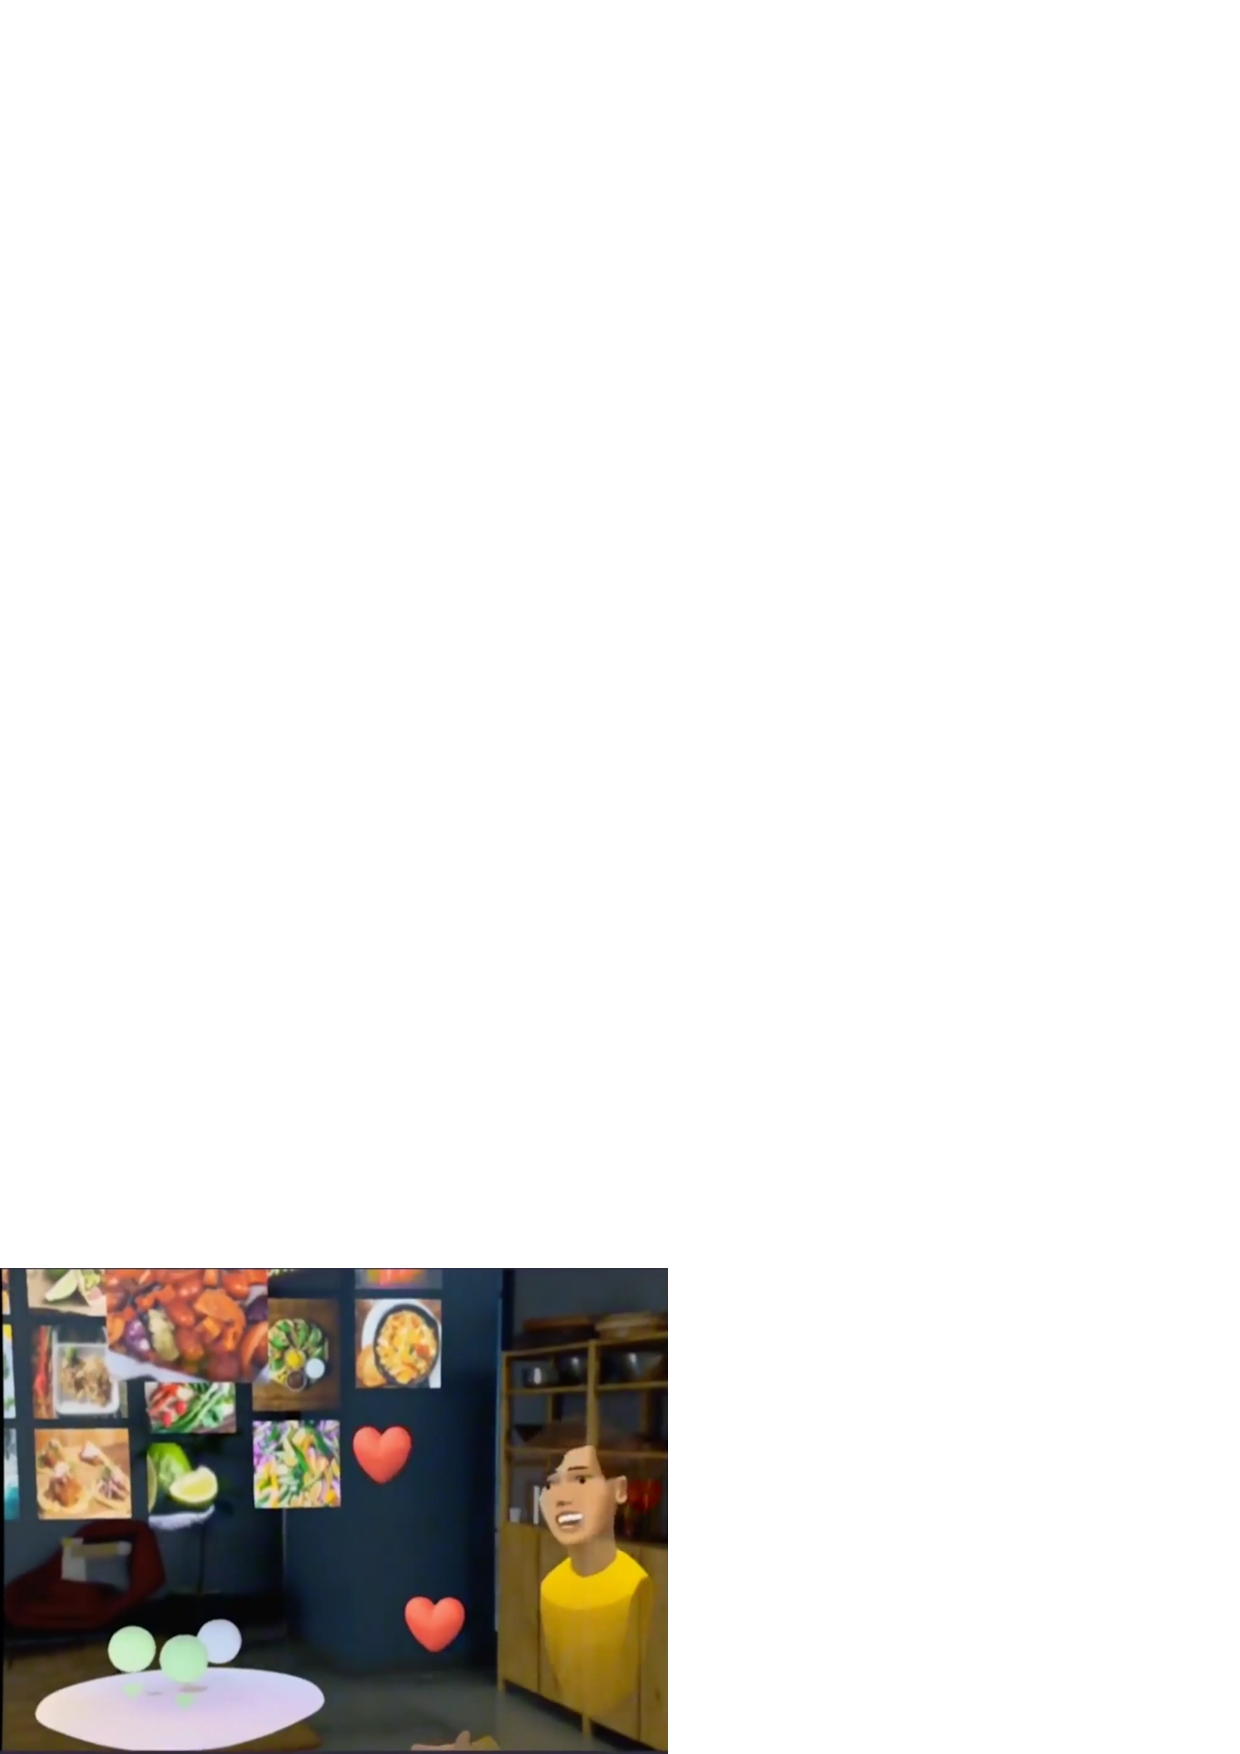
\includegraphics[width=.4\linewidth]{images/avatar-chat-1.png}
    \includegraphics[width=.4\linewidth]{images/avatar-chat-2.png}
    \caption{Example of avatars in AR - Avatar Chat by Magic Leap}
    \label{fig:ml-avatar-chat}
\end{figure}

However, representing social contacts in VR/AR can be cumbersome. It will be more cluttered and overwhelming to represent the data content that social avatars are trying to share. Representing social data has been imagined by futuristic concept videos (e.g., "Hyper Reality"\footnote{https://www.youtube.com/watch?v=YJg02ivYzSs} and "Merger"\footnote{https://www.youtube.com/watch?v=SqW2dEkiD-Y}) where social data can clutter the AR view of the user. It will also raise privacy and ethical concerns.

\cite{Jo2016} studied the influence on co-presence of the background environment (AR vs VR) and the fidelity of the avatar representation of the remote user (photo-realistic vs pre-built). They found that more realistic avatars had a positive impact on the feeling of co-presence between remote collaborators. \cite{Volante2016} also studied the impact of the visual appearance of avatars (realistic vs. stylized) on the inter-personal emotional response of participants. They also found that more visual realism has lower negative affects on the PANAS scale, which measure the intensity of the emotion at a given time. 
Researchers have been investigating social aspects of multi-user VR environments. \cite{Ducheneaut2006} studied massive multiplier online games in terms of social activities, and found that while users may prefer to be with other players, they do not necessarily like actively interacting with them. This led us to think that users may want to have the sense of the presence of social contacts around them, but not necessarily interact with them.

\cite{Harris2009} studied the social behaviour of users of Second Life, and found that users became less active over time and go to familiar places rather than being explorative and actively teleporting/flying. This suggests that people prefer routine and to be surrounded by familiar faces/places over time, forming a social group.

% mark: [you should about how they handle crowds or if everyone is just represented the same] 
However, there has been very little research into social representation in AR. The AR space is more challenging in terms of finding the best locations to fit avatars in the real world so they don't interfere with physical objects or appear suspended in mid-air. However, a social AR application can also allow people to see their friends while doing other tasks; users do not have to use an immersive VR environment to see their social contacts.

Researchers have also explored different ways of managing a large amount of information tags in AR interfaces. \cite{Julier2002} showed how environmental cues, such as distance and user context, can be used to filter AR content into the most relevant information. \cite{Hollerer2001} describe how view management techniques can be used to ensure that virtual objects can be easily seen in collaborative AR interfaces. Similarly \cite{Grasset2012} show how an image-based approach can be used to ensure AR information tags don't overlap in handheld AR. 

This previous research shows that visual fidelity can be used to distinguish between virtual avatars. Different visual representations and spatial cues can also be used to distinguish between information tags in an AR interface. However, there has been little or no research on how to manage social network representations in AR for large numbers of connections. In the next section, we show how visual and proximity cues could be used to organise contacts in a wearable social AR interface.

% \todo[inline]{[In this section you should probably also mention how VR Virtual Avatar environments handle hundreds or more simultaneous users. For example, what tools does second life have for connecting people to hundreds of others. This is directly relevant to your thesis topic]}

\section{Sharing Social Experiences \& Social Networks}

Advancements in mobile phone hardware and increased network connectivity made live video streaming apps popular among smartphone users. Live video streaming apps have been used for sharing social experiences in various contexts. For instance, a person attending a conference or a concert could use her mobile phone to stream the event to her friends and family who could not be there. Similarly, live video streaming apps have also been used for social journalism, turning laypersons into live reporters. Consequently, these apps are now available from different sources with applications such as Periscope\footnote{https://www.periscope.tv/} and Facebook Live\footnote{https://live.fb.com/} among the most popular. These apps allow the users who are sharing to receive comments on the video they are sharing, and to receive simple graphical feedback. 

Common features, such as using the phones' camera which can be either pointed outward (recording what the user sees) or inward (where the user appears in the video), allow users to send a live video stream of what they are doing to hundreds or even thousands of viewers. The purpose of sharing the video is social, so the experience is improved if the viewer can also provide feedback.

\begin{figure}
    \centering
    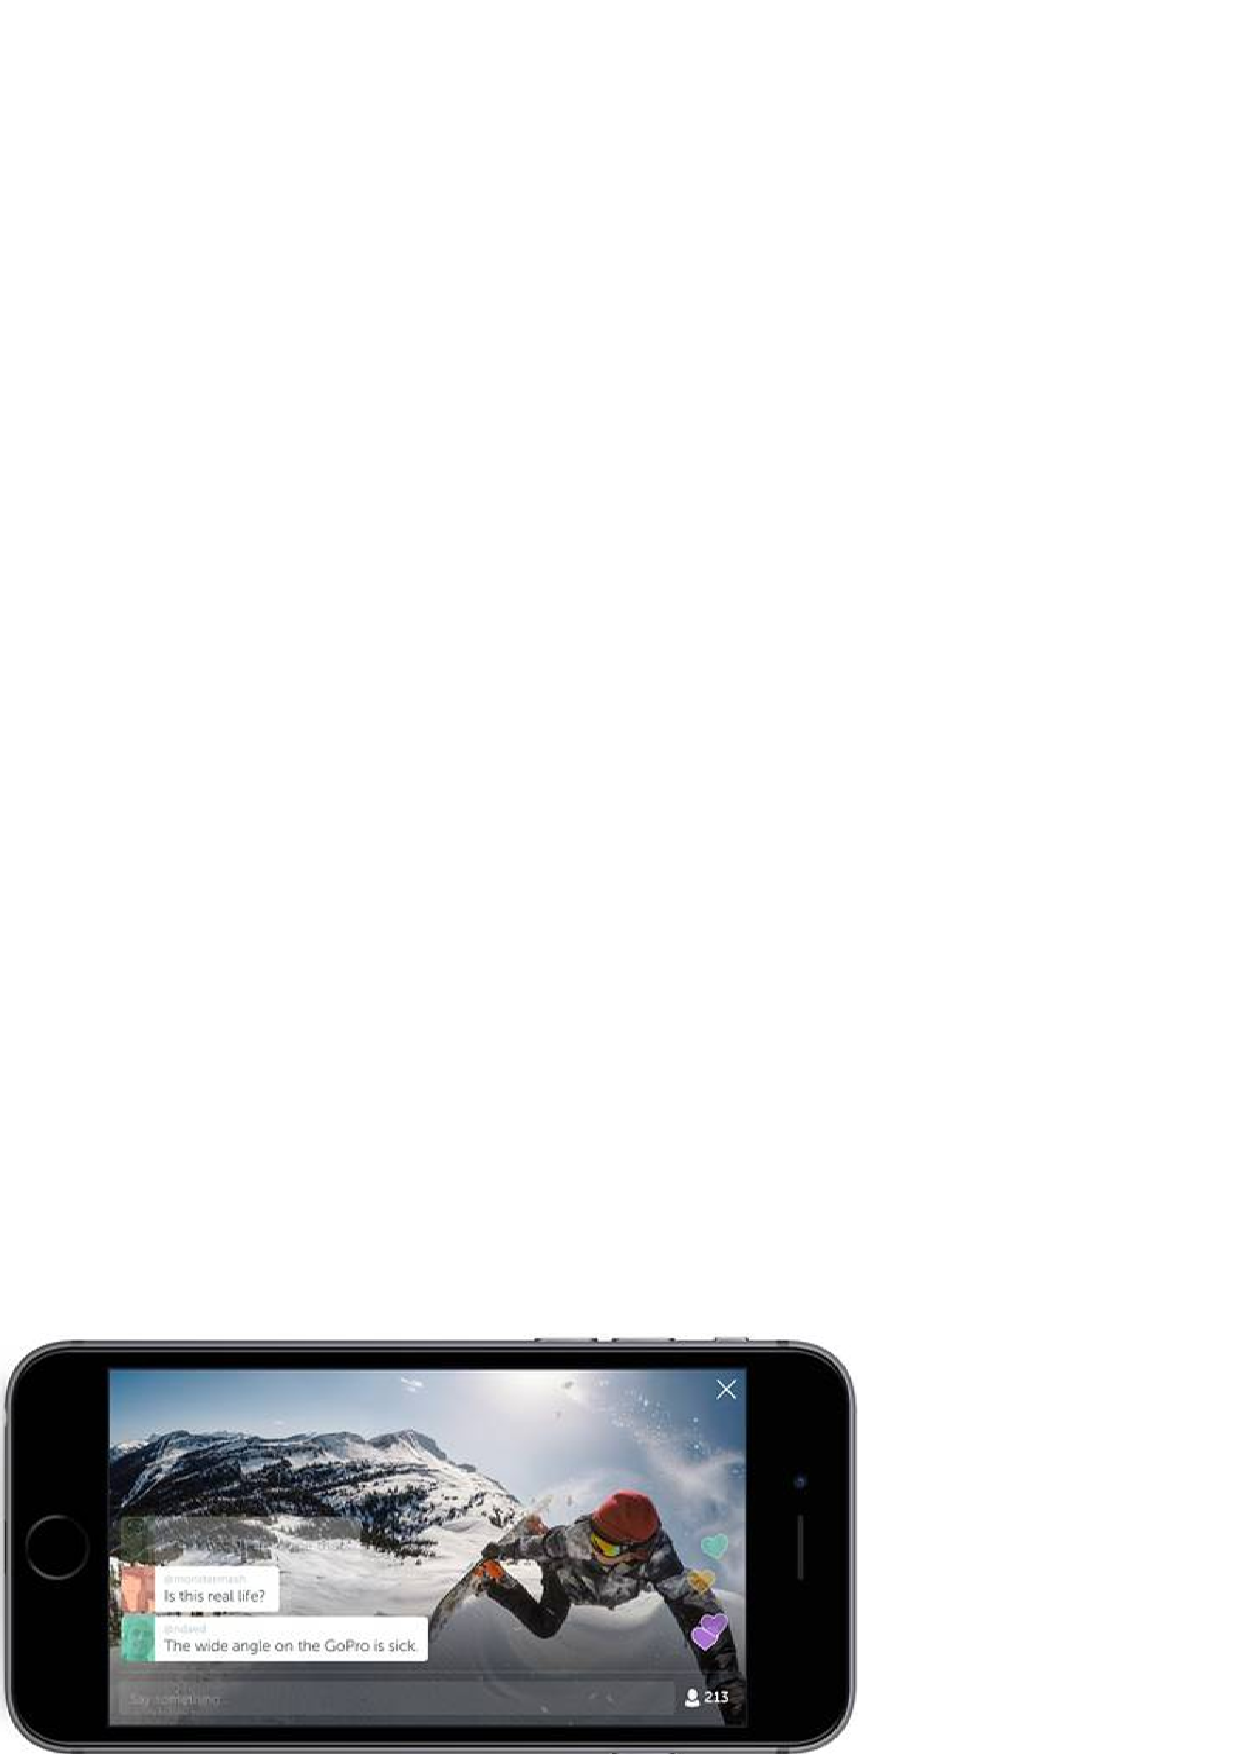
\includegraphics[width=.4\linewidth]{images/periscope.png}
    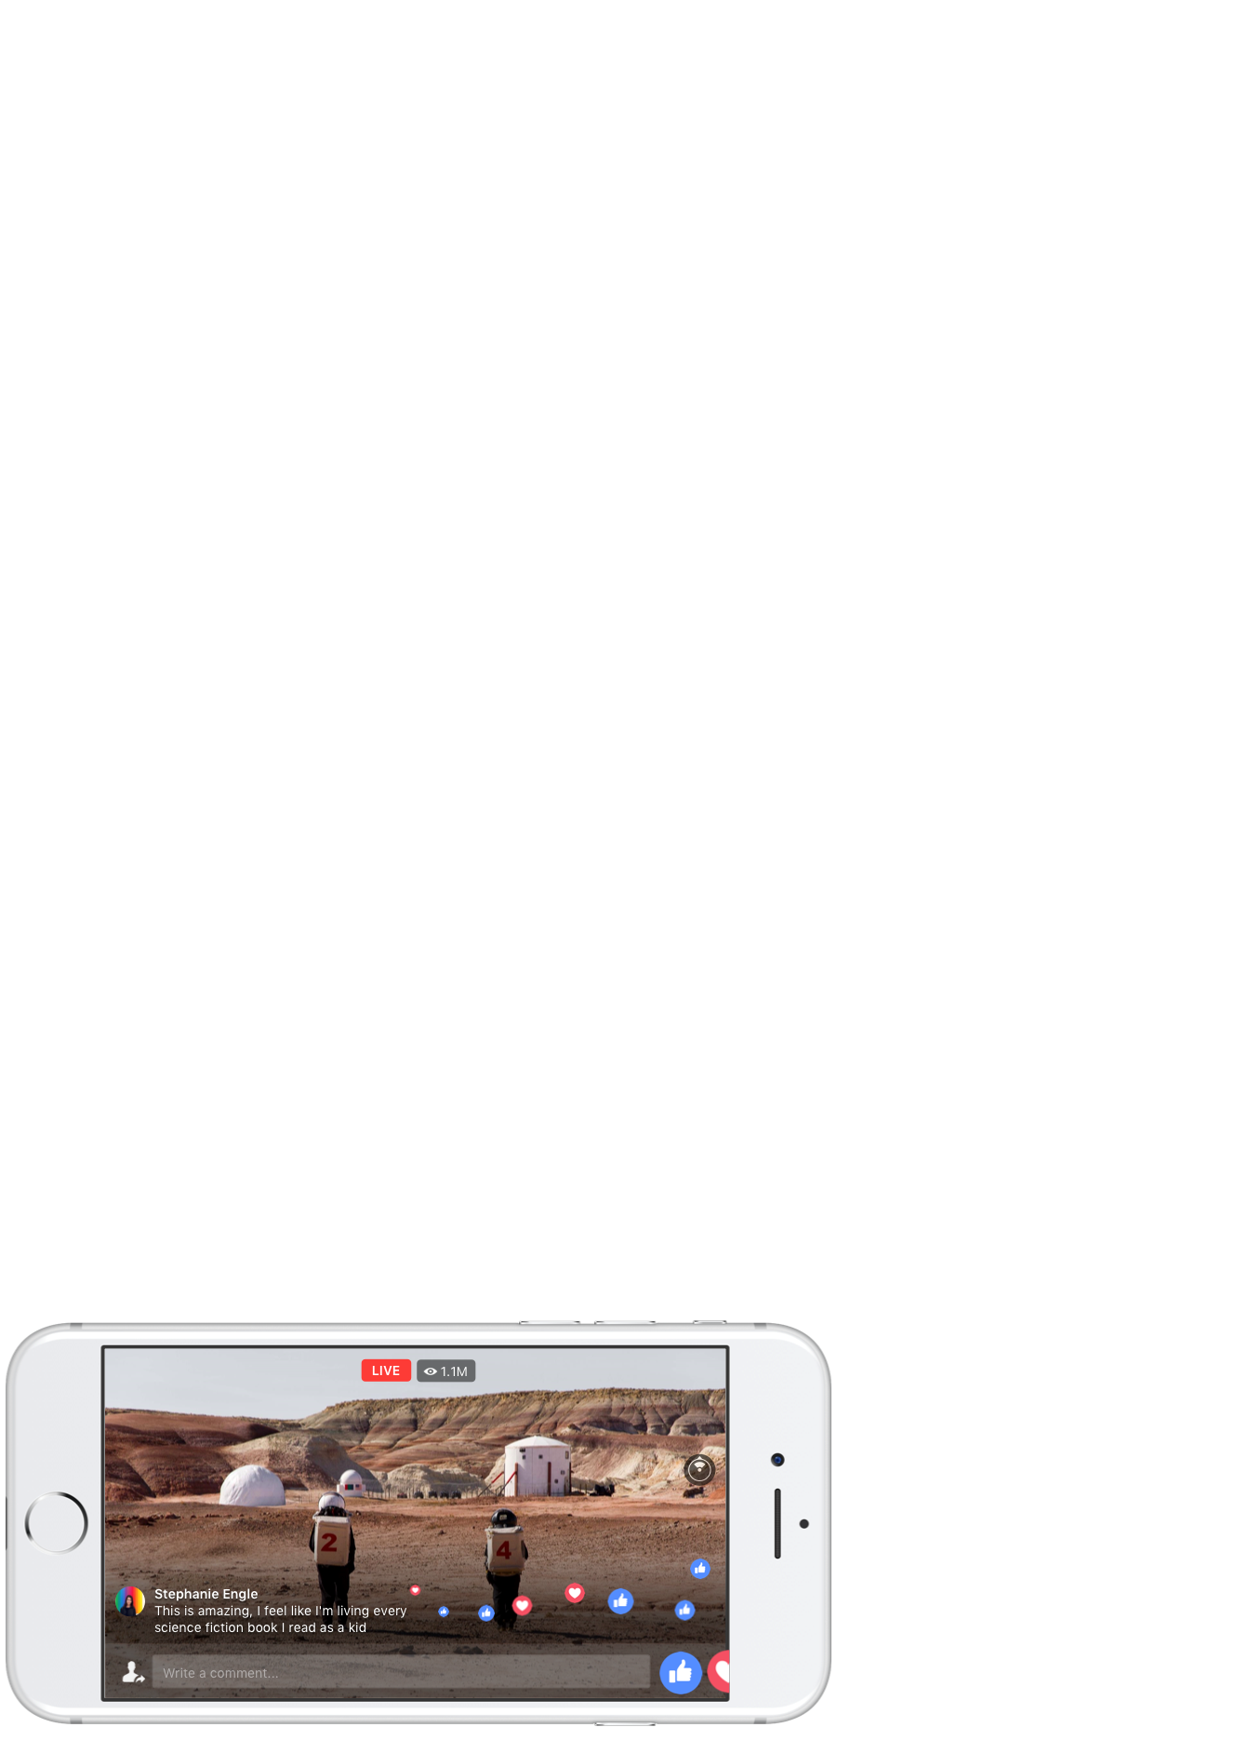
\includegraphics[width=.4\linewidth]{images/facebook-live.png}
    \caption{Examples of live-streaming apps}
    \label{fig:live-streaming}
\end{figure}

In these applications, the feedback comments usually appear in a list below or beside the video being shared (Figure \ref{fig:live-streaming}), separate from the visual context of what the viewer is commenting on. This may cause problems when the person sending the video changes his or her viewpoint. For example, a viewer might send the comment “I really like that view”, but by the time the comment appears, the view might already have changed from the view being commented on.

Future social interactions with wearable AR can be extrapolated from current social network interactions where friends share content and interact with others' content on mobile platforms such as Facebook and Instagram. One trend with mobile social networks is live streaming of a view of a user’s surroundings. For example, Facebook live allows a person with a mobile phone to live stream to remote collaborators. Similarly, wearable AR systems have already been developed that enable people to share a view of their surroundings. For example, the Shared Sphere work of \cite{lee2017mixed} allows a user with a wearable AR display to live stream a 360-degree video of their surroundings to a remote collaborator, although only between pairs of users. 

It is easy to imagine that in the future it will be possible for wearable AR systems to be used to capture and share a 3D view of the user's surroundings with hundreds or thousands of followers on a social network. However, before this becomes commonplace, many important research questions need to be addressed. For example, would a person be comfortable sharing a view of their surrounding real space with relative strangers? This work aims to explore how wearable AR systems could share a user’s surrounding room environment with social contacts and to measure how comfortable the sharer and the viewer would feel regarding privacy within different interface options. 

If AR is to be used to represent contacts in social networks, there could be a large number of contacts to show. Our research has benefited from earlier work on different ways of managing large amounts of information in AR interfaces.


%----------------------------------------------------------------------------------------
%	Summary
%----------------------------------------------------------------------------------------
\section{Summary}

This work aims to layout the space of the AR continuum for social sharing experiences by looking at parameters and options that can be changed in terms of people, objects and the environment to create a shared AR experience. 

Building on previous work on proximity-based relationships \cite{Sousa2016}, we focus on the shared contents of social avatars in an asynchronous situation. Unlike previous work on social avatars, we study representing social contacts in a large-scale network. We aim to reduce the clutter that may be caused by displaying the social avatars and their shared content. We address the question of how we can use the social relationship between avatars and the viewer as a way to filter and enhance viewing the shared-content experiences. 

The scope of this thesis is to explore options of visual user experience design in social AR including displaying contacts, displaying shared data, and displaying shared environments. This thesis does not necessarily cover all possible experiences, but highlights the main points of interactions and reports on user studies measuring the sense of presence and privacy concerns that may occur from these experiences. 

The summary of the trends in the past work is that
% summary of wearable AR 
wearable AR has been the target of many previous developments and research directions. Aiming to enable true outdoor experiences and to be untethered to physical places would allow more exploration of the surrounding world. 
% summary of AR collaboration 
Most of the previous work on AR focused on AR applications for remote collaboration and expert-helper situations. Very few focused on how do we use AR in connecting with our friends and family and for sharing social experiences. Most current commercial applications are focused on expert-helper situations.
% Summary of social AR
In the social aspects of AR, previous work showed few attempts of representing social networks in AR and VR. Also, some applications looked into scanning and using human avatar representations for social connections with others.

The limitation of past work is that it was mainly focused on the remote collaboration of local worker/remote helper situations. However, it did not address sharing social experiences with friends and family scenarios. There is some new work in this area, but not enough to cover all dimensions in this field. The gap that this thesis is addressing is the user interaction design of future wearable AR interfaces so that it can be easily used for sharing social experiences with family and friends. 

This thesis is important because it explores different ways of presenting social networks on wearable AR and helps application designers and developers by providing insights into building similar applications that have a higher chance of being effective and acceptable to users. 

The contributions to the current state-of-the-art are: 1) building software prototypes of sharing social experiences on wearable AR platforms, 2) Running user studies on these prototypes and analysing the results, 3) providing the foundations of the design space of sharing social experiences on wearable AR. 

% \todo[inline]{Gun: You should have a paragraph summarizing the trend in the past work and what is the limitation to support why your work is important. Or you may add a section at the end of this chapter that does an overall review of the whole chapter and describe how your thesis makes contribution to the current state-of-the-art.}

% \todo[inline]{You should end the chapter with a summary of the research gap that you’re going to be addressing.}

% \todo[inline]{[At the end of the related work section you should have a sub-section that provides a summary of the research, particularly highlighting the research gaps and shortcomings of this earlier work. You can then talk about which aspects that you are going to explore further in your PhD thesis. Highlight what is the novelty of your thesis, and what will be the main contributions that your research will make, relative to the earlier related work] }




% \subsection{Sharing for Collaboration}
% \subsection{Sharing for Social}


\chapter{The Social AR Continuum} % Main chapter title
\label{ch:continuum} % Change X to a consecutive number; for referencing this chapter elsewhere, use \ref{ChapterX}

This chapter describes The Social AR Continuum, a space that encompasses different dimensions of Augmented Reality (AR) for sharing social experiences. We explore various dimensions, discuss options for each dimension, and outline possible scenarios where these options might be useful. We categorise the social AR dimensions into three areas: 1) Self and others, 2) Surrounding environment, and 3) Interactions.

Representing self and others as avatars is described in more detail in Chapter \ref{ch:contacts}. The surrounding environment and sharing different types of data is described in more detail in Chapter \ref{ch:data}, while the interactions between people in form of annotation on the surrounding environment is described in Chapter \ref{ch:annotation}.

% \section{Concept}
% \section{General System Implementation}
% \section{Evaluation}

% =============== PREVIOUS WORK ================
% A. Nassani, G. Lee, M. Billinghurst, T. Langlotz, S. Hoermann and R. W. Lindeman, “[Poster] The Social AR Continuum: Concept and User Study” in ISMAR 2017
% =============== PREVIOUS WORK ================

% \section{Abstract}
% \label{sec:continuum-abstract}

In this work, we describe The Social AR Continuum, a space that encompasses different dimensions of Augmented Reality (AR) for sharing social experiences. We explore various dimensions, discuss options for each dimension, and explore possible scenarios where these options might be useful. We describe a prototype interface using the \textit{contact placement} dimension, and report on feedback from potential users which supports its usefulness for visualising social contacts. Based on this concept work, we suggest user studies in the social AR space, and give insights into future directions. 

\begin{figure}
    \centering
    \includegraphics[width=3in]{images/continuum_categories5.png}
    \caption{The social AR continuum categories: 1) self and others, 2) objects and surrounding environments, 3) interaction and annotations}
    \label{fig:continuum:categories}
\end{figure}


% \section{Introduction}

% With wearable Augmented Reality (AR) devices becoming affordable, available and ubiquitous, there is a need to understand design considerations for this new platform. Previous research has looked into using AR headsets for collaborative use. The research presented here explores the use of AR headsets for social interaction and shared experiences. Social interactions can be extrapolated from current social network interactions where \enquote{friends} share content and interact with another's content (i.e., likes, comments).

% In the social AR/VR space, previous work implemented visual representations of self and others (e.g., Facebook Spaces\footnote{https://www.facebook.com/spaces}) to create fun overlays and representations of the face and upper body. In other research, \cite{Fanello2016} prototyped live sharing of a full scan of a person's body with remote users using 3D cameras and the HoloLens\footnote{https://www.microsoft.com/en-nz/hololens}. For representing “people” in AR space, \cite{Sousa2016} studied the concept of \enquote{personal space} and \enquote{social bubbles} in terms of proxemic interactions between people in different places. They used floor projections and hand-held devices to communicate the presence of remote people. They also established a \enquote{gradual engagement model for remote proxemic} based on distance from the user which consists of 1) personal, 2) engaged, 3) peripheral, and 4) ambient.

% Most work has focused on how visual representation and proximity could be used to organize an AR representation of a person's social network. However, this information could also be used to modify the contextual information being shared by a user out to their social network as well. For example, a person may not want strangers to know what they look like, and so would prefer being represented as a stylistic icon to people that do not know them, but would be more comfortable sharing a lifelike representation to those that are close to them. 
 
% In many mobile AR applications, the technology is used to share a view of the user's world. For example, remote expert collaboration systems have been developed where a local worker with an AR display can share a live video view of their workspace with a remote expert \cite{Billinghurst2002}. The remote expert can provide visual feedback with AR graphical cues.

% When people connect in this way, they may also want to share different amounts of information about their surroundings with each other. For example, users who are close in a social network may be happy to share a 3D virtual view of their surroundings and have the remote user appear as an AR avatar in their real space, while those that are strangers may only want to have an audio connection and not show anything of their surroundings to preserve their privacy but allow them to share and control their privacy \cite{Oetzel2011}. The position on the social continuum could be used to modify how much information a person can share about themselves and their surroundings.

This work aims to layout the space of the AR continuum for social sharing experiences by looking at parameters and options that can be changed in terms of people, objects and the environment to create a shared AR experience. This is still work in progress, but aims to cover all dimensions of the AR continuum.

\section{Social AR Continuum Dimensions}

As we established the social AR continuum varies based on the closeness of social connections that we have with others (relationship), we identified the following dimensions where social AR applications can fit along a continuum. The dimensions can be grouped in the categories described in Figure \ref{fig:continuum:dimensions}.

% \begin{figure}
%     \centering
%     \includegraphics[width=3in]{images/dimensions-diagram-01.eps}
%     \caption{Dimensions of Social AR Continuum.}
%     \label{fig:continuum:dimensions}
% \end{figure}


\begin{figure}
    \centering
    \includegraphics[width=3in]{images/continuum.eps}
    \caption{Dimensions of Social AR Continuum}
    \label{fig:continuum:dimensions}
\end{figure}

\textbf{Contact Representation}
Representing social contacts can vary on the social AR continuum based on the relationship that the user has with the contact. Intimate contacts can be represented as full 3D animated avatars. Friends could be represented as 2D static images, while Acquaintances could be represented as 2D busts, and strangers as merely emojis. Each contact could choose their own representation for each category.  

\textbf{Contact Filter}
Filtering social contacts to distinguish users from each other could be done using proximity or visual fidelity based on their relationship to the user. Proximity filters contacts by placing them closer or further-away. Visual fidelity filters contacts by adding more level of detail to the contact for closer relationships and less detail for further away contacts. 

\textbf{Contact Placement}
Placing social contacts can be done either by displaying them as life-size avatars on the ground around the user for close relationships, or by displaying them as miniatures on a distant surface. 

\textbf{Data Type}
The type of data shared between social contacts in AR can be categorised as 1D (e.g., text or audio), 2D (e.g., images, panorama or video), or 3D (e.g., 3D model or scanned-room environment). Based on the relationship between the user and his/her social contacts, the type of data available can be filtered. For instance, 3D data are shared with intimate relationships, while acquaintances can see only 2D data.  

\textbf{Data Interaction}
In terms of user interactions with shared data, the continuum here ranges from viewing the contents, annotating or adding comments on the content, through to manipulating the content. Levels of manipulation include changing the position, rotation or scale of the shared content, or even modifying the content itself

\textbf{Data Privacy}
Based on relationship with other users, shared data can be made private to the user, shared with specific groups of people (e.g., friends, acquaintances), or shared with everyone. 

\textbf{Sync/Async}
The data shared with contact can be shared in a synchronous way where both sharing and interaction happen at the same time. In contrast, data can be also shared asynchronously \cite{Smith2016} i.e., interaction happens at a different time. 

\textbf{Co-location}
Social contacts can either be remote (i.e., in a different place than the user) or face-to-face (i.e., physically in the same location as the user). When social contacts are remote, they are represented as virtual avatars based on their relationship with the user. An example of face-to-face interaction was described in a Black Mirror \footnote{http://www.imdb.com/title/tt2085059/} episode where a person could 'block' another co-located person by blurring them out in their AR view of the real world.

\section{Summary}

In this work, we introduced the concept of The Social AR Continuum. We identified several dimensions where a social AR application could be implemented. We created a prototype interface on one dimension -Contact Placement- comparing life-size to miniature avatars. From the collected data we found that both conditions were well received by potential users. In the future, we plan to explore other dimensions, study the effects of avatar realism, and report on users' perception of the continuum.


\chapter{Annotation Continuum} % Main chapter title
\label{ch:annotation} % Change X to a consecutive number; for referencing this chapter elsewhere, use \ref{ChapterX}

This chapter studies the social AR continuum in term of interactions between users. The interaction is represented by annotation or adding an AR tag on shared medium to socially connect with other users. The first section \ref{sec:video} addresses annotation on live video streaming medium. The second section \ref{sec:3D} studies the annotation on a 3D environment using 3D sensors to detect the shared surrounding environment. 


\section{AR Annotation on Social Video Sharing}
\label{sec:video}
% =============== PREVIOUS WORK ================

% A. Nassani, H. Kim, G. Lee, M. Billinghurst, T. Langlotz, and R. W. Lindeman, “Augmented reality annotation for social video sharing,” in SIGGRAPH ASIA 2016 Mobile Graphics and Interactive Applications on - SA '16, 2016, pp. 1–5.

% =============== PREVIOUS WORK ================


% \subsection{Abstract}

This paper explores different visual interfaces for sharing comments on a social live video streaming platforms. So far, comments are displayed separately from the video making it hard to relate the comments to event in the video. In this work we investigate an Augmented Reality (AR) interface displaying comments directly on the streamed live video. Our described prototype allows remote spectators to perceive the streamed live video with different interfaces for displaying the comments. We conducted a user study to compare different ways of visualising comments and found that users prefer having comments in the AR view rather than on a separate list. We discuss the implications of this research and directions for future work.

% \subsection{Introduction}

% Advancements in mobile phone hardware and increased network connectivity made live video streaming apps popular among smart phone users. Live video streaming apps have been used for sharing social experiences in various contexts. For instance, a person attending a conference or a concert could use her mobile phone to stream the event to her friends and family who could not be there. Similarly, live video streaming apps have also been used for Social journalism turning laypersons into live reporters. Consequently, these apps are now available from different sources with applications such as Periscope\footnote{https://www.periscope.tv/} and Facebook Live\footnote{https://live.fb.com/} among the most popular apps. 

% They all share common features such as using the phones' camera which can be either pointed outward (recording what the user sees) or inward (where the user appears in the video) and allowing users to send a live video stream of what they are doing to hundreds or even thousands of viewers. The purpose of sharing the video is social, so the experience is improved if the viewer can also provide feedback. Applications like Periscope allow the users who are sharing to receive comments on the video they are sharing as well as they can receive simple graphical feedback. 

% In these applications, the feedback comments usually appear in a list below or beside the video being shared, separate from the visual context of what the viewer is commenting on. This may cause problems when the person sending the video changes his or her viewpoint. For example, a viewer might send the comment “I really like that picture”, but by the time the comment appears, the view might already have changed from the picture being commented on.

In this work, we investigate how comments can be displayed for a live video sharing experience using a mobile device, and especially focus on using Augmented Reality (AR). We implemented three different interfaces to display comments: (1) List, (2) Augmented Reality (AR), and (3) List + AR (see Figure \ref{fig:mgia16:conditions}). In the rest of the paper, we first describe earlier research, then our prototype implementations, and finally a user evaluation comparing the three different methods. 

\begin{figure}
  \includegraphics[width=\columnwidth]{images/mgia16/screenshots-enhanced}
  \caption{Overview on the investigated interfaces showing screenshots of the different interface conditions. (L) List: Comments displayed as a list on the side. (AR) AR: Comments displayed over the background video. (L+AR) List+AR: Comments displayed both as a list on the right and over the background video. }
  \label{fig:mgia16:conditions}
\end{figure}

% \subsection{Related Work}

Our work extends earlier work on live video sharing on mobile devices and different types of interfaces for showing feedback from the viewers. 

% Current popular live video sharing apps, such as Periscope, or popular live streaming websites  such as Douyu\footnote{http://www.douyu.com/} and Ingkee\footnote{http://www.ingkee.com/} use a single way of displaying comments from other users. The common method is to display comments as a list either beside or below the shared video or sometimes floating on top of the video from left to right. This approach is a good extension of standard chat applications. However, it may not be the best for sharing a video from a hand-held device; the sharing person is moving the device and therefore the camera view could be different when the comments arrive. 

 
% TODO: [it would be good to add more detail here and also several more references. There must be other papers on video commenting?]

% Other research has looked into adding comments on video by analyzing the video content \cite{LaiolaGuimaraes2012}. Kim \textit{et al.} \cite{Kim2013} have explored how spatially aligned drawing on a live AR view can improve remote collaboration. However this did not include live text comments. Some researchers have explored how to easily add text and graphic annotations to recorded videos on mobile devices. For example MoVia \cite{Cunha2013} allows people to draw on or add text tags to recorded video that can then be shared asynchronously. However the focus of applications like this is on annotation and not real time social sharing or live streaming. 

% TODO: [you could include other examples] -- after Kim paper

% One of the few examples of previous research into annotation on live video streamed from a mobile platform is the work of Huang \cite{Huang2012}, who developed a system for adding text or drawing onto a live camera view and sharing it with a remote user. However in this case their research was focusing on the system performance and not an evaluation of the interface usability. The interface also did not support real time comment feedback and was not focusing on social networking.  

In our research we want to place comments in a spatially aligned AR view on top of the live video feed. Using spatially aligned AR to add content to the real world is not a novel idea. For example, \cite{Langlotz2013} used GPS coordinates to determine the position of a sound and positioned them spatially around the user. Similarly the AR browser applications Junaio\footnote{junaio.com, unavailable since 2015. Acquired by Apple} and Sekai Camera\footnote{sekaicamera.com, unavailable since 2014. Evolved to http://tab.do/} allowed users to add AR comments in the real world. However, to our knowledge, no previous research on methods for commenting on live video has been done. Spatially aligned comments or annotations can benefit from understanding the surrounding 3D environment. For example, \cite{Nassani2015} implemented AR tagging using Google Tango to track from the environment, and Google Glass to display AR comments, however this did not support real time video sharing. 
% TODO: Mark: (about Tobias paper above) In this case they are adding audio annotation, so I'm not 100% sure how relevant this is.

Although previous work has demonstrated live video sharing on a mobile platform and support for viewer feedback, there has been little evaluation of different methods for providing feedback. In this paper, we report on investigations into different user interface (UI) options for viewing comments left by multiple users on a shared live video stream. Thus, the main contribution of the work is investigating if comment placement on live video sharing improves the user experience. In the next section we describe the prototype developed to explore this question.

\subsection{System Design}

We developed a prototype that enables a user to share a live video stream with others and receive comments from multiple users watching. Our system consists of a WebRTC\footnote{https://webrtc.org} application running on AppEngine\footnote{https://appengine.google.com/} on Google Cloud servers, which offers a fast peer-to-peer connection between devices. Being built on a web platform, this solution can run on multiple hardware specifications including desktop, hand-held, and wearable devices. Figure \ref{fig:mgia16:system} shows the overall design of the prototype system.

% TODO: explain the diagram more 
\begin{figure}[ht]
  \centering
  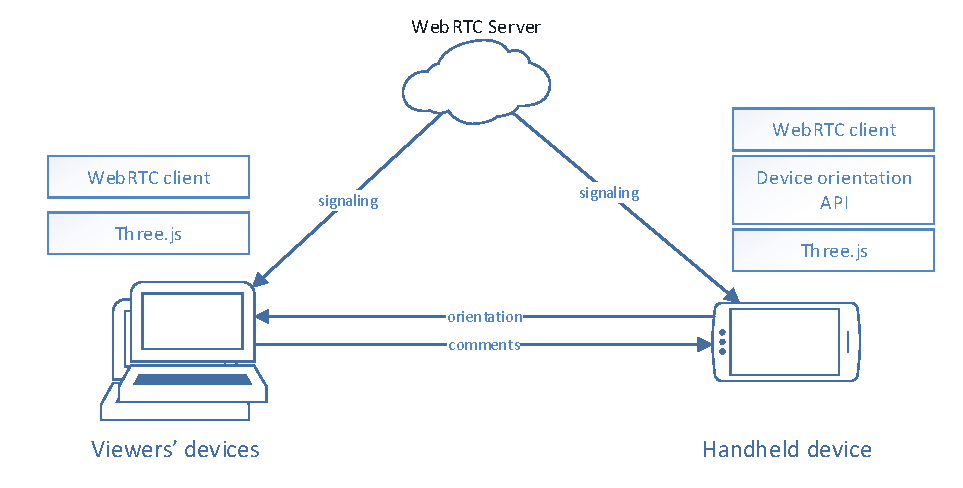
\includegraphics[width=3in]{images/mgia16/system}
  \caption{System architecture based on WebRTC}
	\label{fig:mgia16:system}
\end{figure}

The prototype was built on top of AppRTC\footnote{https://apprtc.appspot.com/} which hosts a website that enables people to start a video conferencing session on the web. To support AR visualization of comments, we utilized the AppRTC code to track device orientation by listening to the device sensors. The AppRTC application is written in Python for the backend and Javascript for the front-end. It takes advantage of being hosted on AppSpot so that it complies with the WebRTC requirements for HTTPS. The AppRTC system allows users to communicate with each other over the Internet. In addition to the video stream, we modified the code to transfer the device orientation data to the receivers' devices via DataChannel. To render comments in the AR visualization, we used the Three.js library\footnote{http://threejs.org/}. The AR visualization is implemented with two graphical layers. The background layer shows the video stream captured by the camera on the mobile device. On top of the background, comments are drawn on the front layer using orientation tracking information to show them in a body-stabilized manner \cite{Billinghurst1998}. 

\subsection{Implementation}

The application starts by turning on the back camera on the mobile device. It then asks the user to enter a “room number” to start the connection. Once this is entered, the application will start a call mode, waiting for other participants to enter the same the room number. Once the call is established, the mobile device will start streaming video and device orientation data to the viewing PC. 

Both users can send comments to each other by clicking on any part of the shared video. The system then calculates the 3D position of the comment in the AR space and waits for the comment text to be entered. Once the user enters the message, the text is displayed on both the sender's and receiver's screens. The motion data of the sender's device is also shared so that the receiver will see the comment appearing at the same place as the sender turns his/her device. 

Three different ways of showing comments on the live video stream were implemented. A list view where the comments are listed on the side of the camera feed view. An AR implementation (AR) where the comments were overlaid on top of the video feed and rotated around the user based on phone orientation, so the comments appear fixed at the location on the video where they were first entered. Finally, an AR + list implementation combined the list view with the AR view. In the next section, we report on a user study exploring these three implementations.

\begin{figure}[ht]
  \centering
  \includegraphics[width=3in]{images/mgia16/participant2}
  \caption{Comment appearing on top of the shared video}
	\label{comments}
\end{figure}


\subsection{User Study}

We conducted a controlled within-subjects user experiment to test the different user interfaces for displaying comments. There were three conditions: L) comments in a list, AR) comments on the video with AR visualization, and L+AR) comments on both. The experiment started with the participants giving consent and answering questions about demographic information. Then they went through a training session to get familiar with the application and the experimental procedures.

To simulate different environments for the user, we used 180-degree panoramic images projected around the user on large screens to simulate different real spaces (see Figure \ref{fig:mgia16:participant}). We selected four different images where the user might be interested in sharing his or her surroundings, varying in terms of indoors/outdoors and busy/quietness. A different background was randomly assigned for each condition between subjects. 

\begin{figure}[ht]
  \centering
  \includegraphics[width=3in]{images/mgia16/participant1}
  \caption{Participant during the experiment}
	\label{fig:mgia16:participant}
\end{figure}

Each participant was asked to sit in the middle of the projection screens showing the background image, hold a smart phone, and aim its camera at the background to share it with remote users. The experimenter simulated multiple users sending comments on the shared video in a ‘Wizard of Oz' style setup. There were six predefined comments for each background. The comments appeared on the screen in three different styles depending on the experimental condition. The order of the conditions was counterbalanced using a balanced Latin square design. While watching the comments, the participant was asked to remember which part of the background each comment was talking about and who made the comment, which could be identified by the colour of the comment. There were up to four colours (commenters) in the experiment. The comments faded away one minute after being displayed. This was to simulate the user receiving multiple comments while having limited time to read them all.


After completing a condition, participants were asked to place a printed version of each comment on a background image, at the correct location, and with the correct colour, testing their knowledge of where each comment appeared. The participants were also requested to answer a questionnaire on system usability \cite{brooke1996sus} and social presence \cite{Harms2004}. The questions were slightly modified to fit the scenario being tested and only focused on one-way communication. Table \ref{table:social_questions} shows the social presence questions that were answered on a seven-level Likert scale rating (1: strongly disagree - 7; strongly agree). 

\begin{table}[h]
  \centering
  \caption{Social presence questionnaire. Negative questions marked with (-)}
  \label{table:social_questions}
  \begin{tabular}{lll}
    Q1 & Comments from others were clear to me.          \\
    Q2 & It was easy to understand comments from others. \\
    Q3 (-) & Understanding others' comments was difficult.  \\
    Q4 & I could tell how others felt by my video sharing.\\
    Q5 (-) & Others' emotions were not clear to me.\\
    Q6 & I could describe others' feelings accurately.
  \end{tabular}
\end{table}

% [do you want to show system usability questions as well?]

After finishing all three conditions, participants answered a post-experiment questionnaire that asked them to rank and compare all three conditions in terms of strengths and weaknesses. Finally, the experiment ended with a debriefing and the opportunity for participants to provide open-ended comments.

\subsection{Results}

We recruited 20 participants (11 female, aged between 19 and 35 years old, Median=27.5, SD=4.55). Most (95\%) of them had experience with live video streaming a few times a week to a few times per month and 80\% were familiar with AR applications. We used a non-parametric Friedman test for all the results with alpha=0.05, and post-hoc tests using Wilcoxon signed-rank tests with the Bonferroni correction (alpha=0.017)

The statistical result for SUS (see Figure \ref{fig:mgia16:questions_sus}) showed that there was a statistically significant difference between conditions ($X^2(2)=9.658, p=0.008$). Post-hoc analysis showed significant differences between L and AR (Z=-2.638, p=0.008) and between L and L+AR (Z=-2.559, p=0.010). However, there was no statistically significant differences between AR and L+AR (Z=-0.197, p=0.844). This shows that the list condition on its own was considered considerably less usable than the other two conditions.


\begin{figure}[ht]
  \centering
  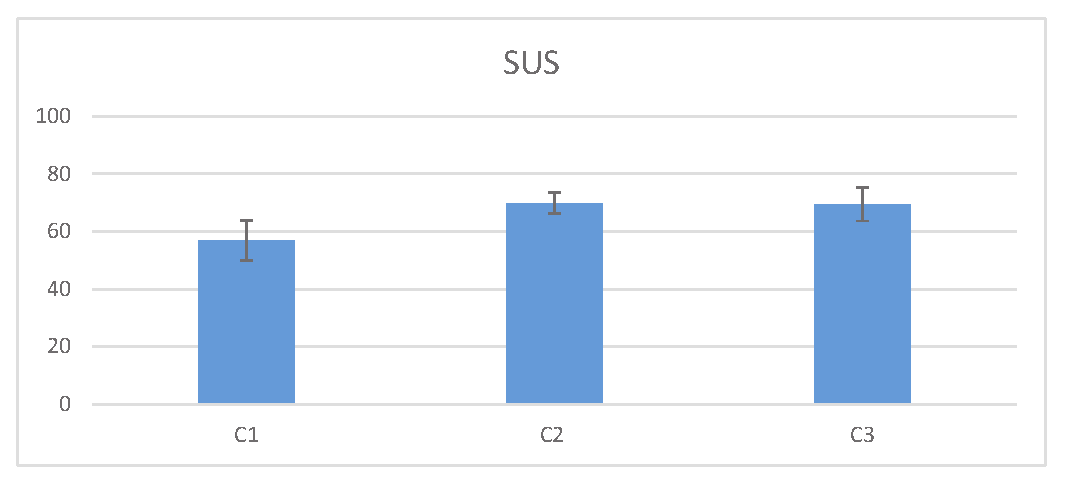
\includegraphics[width=2.5in]{images/mgia16/sus.eps}
  \caption{SUS score}
  \label{fig:mgia16:questions_sus}
\end{figure}

As for the social presence questions (see Figure \ref{fig:mgia16:social_presence}), we inverted the responses on the negative questions Q3 and Q5, to allow all questions to be aggregated, combining the answers for both perceived message understanding and affective understanding. There was a statistically significant difference in perceived social presence ($X^2(2)=16.892, p<0.001$). Post-hoc analysis found there were significant differences between L and AR (Z=-3.459, p=0.001) and between L and L+AR (Z=-3.311, p=0.001) while there was no statistically significant difference between AR and L+AR (Z=-0.427, p=0.670). This shows that the list condition (L) was perceived as being less easy to understand, and that viewer comments in this condition were less clear.

\begin{figure}[ht]
  \centering
  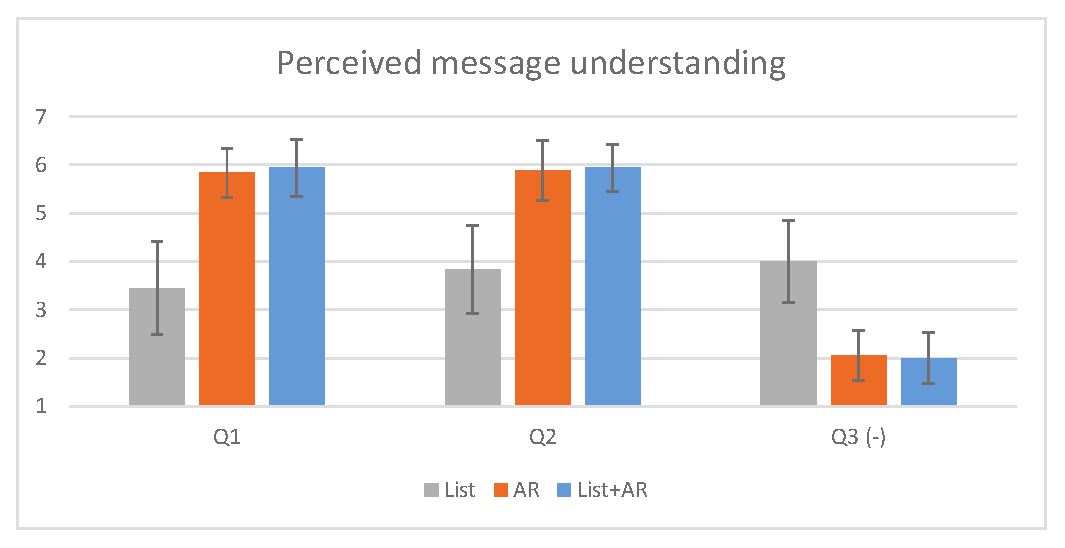
\includegraphics[width=2.5in]{images/mgia16/message.eps}
  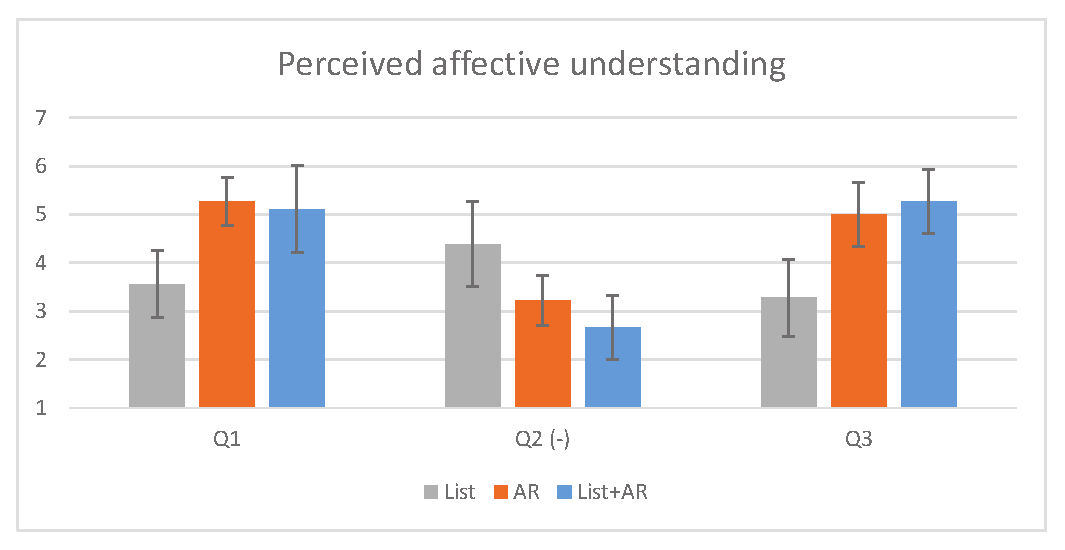
\includegraphics[width=2.5in]{images/mgia16/affective.eps}
  \caption{Results for the social presence questions "perceived message understanding" and "perceived affective understanding"}
	\label{fig:mgia16:social_presence}
\end{figure}

As for the ranking results (see Figure \ref{fig:mgia16:ranking}), we calculated the average of the answers (where 3=highest ranking, 1=lowest ranking). The results show a statistically significant difference between conditions ($X^2(2)=9.100, p=0.011$). Post-hoc analysis showed a significance level set at $alpha$=0.017. There were significant differences between L and AR (Z=-2.766, p=0.006) and between L and L+AR (Z=-2.502, p=0.012). However, there was no statistically significant difference between AR and L+AR (Z=-0.039, p=0.969). This shows that the list condition (L) was ranked the worst out of the three conditions.

\begin{figure}[ht]
  \centering
  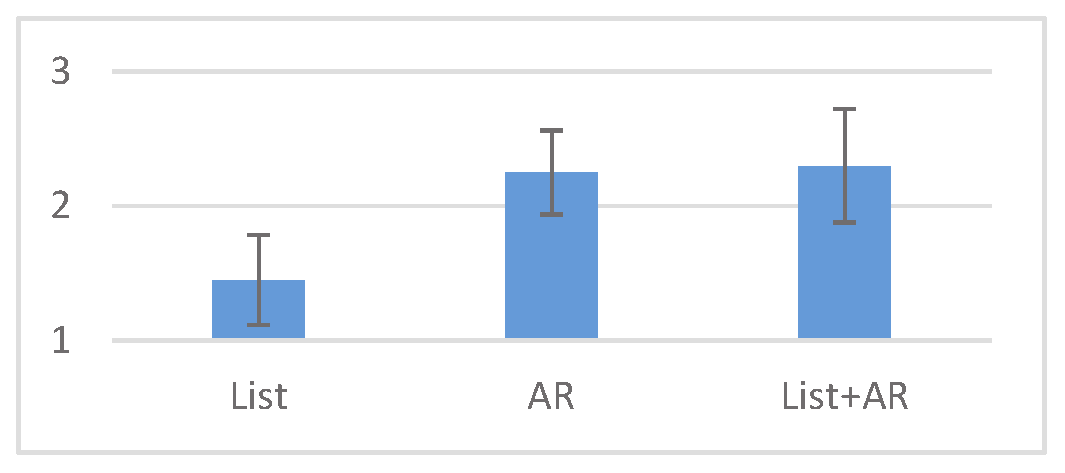
\includegraphics[width=2.5in]{images/mgia16/ranking.eps}
  \caption{Results for conditions ranking questions}
	\label{fig:mgia16:ranking}
\end{figure}

For the task of matching the position and colour of the comments (see Figure \ref{fig:mgia16:questions_matching}), The results show that there was a statistically significant difference ($X2(2)=22.030, p<0.001$). Post-hoc analysis showed that there was no significant difference between the L and AR conditions (Z=-1.016, p=0.310). However, there was a statistically significant difference between L and L+AR (Z=-3.628, p$<$.001) and between AR and L+AR (Z=-3.447, p=0.001).

\begin{figure}[ht]
  \centering
  \includegraphics[width=2.5in]{images/mgia16/matching.eps}
  \caption{Results for correctly matching comments with background and colour.}
	\label{fig:mgia16:questions_matching}
\end{figure}

Participants were asked free-form questions to comment on their experience in terms of the strengths and the weaknesses of each condition. Approximately 80\% of feedback from the participants noted that in the list condition (L) it was more difficult to identify the area of the comments comparing to the AR conditions. Eight participants (40\%) found it more challenging to remember the comment colours as a means to identify the person who sent the comment. 

In the AR and L+AR conditions participants felt that the comments were contextual and relevant to the background. For example, \textit{"It's easier to remember comments on video (AR) because the comments acts as cues on the video you can directly see what the people are commenting on which I think makes me feel more connected to them"}. One of the strengths of the L+AR condition commented on included having an overview of the list of comments even if they are outside the current viewpoint of the user. 

However users felt that comments in the L+AR condition could clutter the UI and partially block the background. One participant said \textit{"The screen just became too busy with comments that I don't have the time to actually sort out the comments and associate them on the video"}. Some suggested this could be resolved by making the comments not in the center of view more transparent.
 
We asked the participants what would they like to improve. Most reported that they would like to use a head-mounted display to view comments in the AR mode.  It was also suggested that we use a profile image instead of colours on comments to distinguish remote users.
 
Overall users felt that the AR and L+AR conditions were fun and cool to use, providing comments such as \textit{"It's pretty awesome. I love the experience and I would really like to use this app with my social network."}.


\subsection{Discussion}

From the user study, we found that subjects preferred the conditions that contained an AR view, compared to showing comments only displayed in a list format. They thought these conditions were more usable, provided a higher degree of social presence, and enabled them to better remember the comment layout. This is probably because the spatial association of comments increases the likelihood of the message being understood and being attended to.

We expected that one of the AR conditions (AR or L+AR) would have been more popular than the other, however this was not the case. Some users preferred L+AR over the AR as the former provided an overall list of comments even if they were not visible in the current user viewpoint; making the user more aware of new comments without needing to look around to find them. Other users preferred the AR only condition, as the screen is less crowded. One solution to this might be by hiding the comments on the list that are visible on the AR view, removing any duplication. Alternatively we could use a radar view that shows dots to represent comments. 

We learned more about how to make the live streaming a better experience for the user. Some users found the one-minute timeout for the comments fading away to be too fast. Associating the comments with colour to represent different users may not be the best option. An alternative approach would be to use an avatar or name of the person to identify the comment source. 

The study has a number of limitations that we will have to address in the future. The experiment was conducted in a simulated environment rather than outdoors. We also used a static background image to simplify the conditions. However in real life, things will be moving in the background (i.e. people walking, cars passing by). In such scenarios, the comments in the AR condition may not stick to the moving objects. However, this could be solved by using image processing techniques to track objects that will allow the comment to be moved with them. Finally, the all of the comments were generated by an experimenter and were fixed, rather than coming from real people who could write whatever they liked.    

\subsection{Summary}

In this paper, we investigated AR annotations for social live video streaming. We conducted a user study testing three variations of the interface for showing comments: 1) a list, 2) an AR view and 3) both list and AR views. Participants felt that the AR and the List + AR conditions were significantly better than the List condition in terms of system usability and social presence. This was probably because the spatial alignment of comments increases the likelihood of them being understood and attended to.

In the future, we plan to investigate alternative mechanisms for communicating in a social live video sharing sessions, such as using sketching or emojis. We will also explore how depth cameras could be integrated into the system to enrich the social sharing experience by providing improved tracking and environment recognition. Finally, we would like to conduct more extensive user studies that test various user interface designs for using AR for sharing social experiences. This could include being able to navigate back in time to see comments before. 



\section{AR Annotation using 3D sensors}
\label{sec:3D}

% =============== PREVIOUS WORK ================

% A. Nassani, H. Bai, G. Lee, and M. Billinghurst, “Tag it!: AR annotation using wearable sensors,” in SIGGRAPH ASIA 2015 Mobile Graphics and Interactive Applications on - SA '15, 2015, pp. 1–4.

% A. Nassani, H. Bai, G. Lee, and M. Billinghurst, “Extending HMD by chest-worn 3D camera for AR annotation,” in SIGGRAPH ASIA 2015 Mobile Graphics and Interactive Applications on - SA '15, 2015, no. Figure 2, pp. 1–2.

% =============== PREVIOUS WORK ================


% \subsection{abstract}

In this work we describe a wearable system that allows people to place and interact with 3D virtual tags placed around them. This uses two wearable technologies: a head-worn wearable computer (Google Glass) and a chest-worn depth sensor (Tango). The Google Glass is used to generate and display virtual information to the user, while the Tango is used to provide robust indoor position tracking for the Glass. The Tango enables spatial awareness of the surrounding world using various motion sensors including 3D depth sensing, an accelerometer and a motion tracking camera. Using these systems together allows users to create a virtual tag via voice input and then register this tag to a physical object or position in 3D space as an augmented annotation. We describe the design and implementation of the system, user feedback,  research implications, and directions for future work.  


% \subsection{Introduction}


% In our research we are interested in allowing people to place virtual tags at points or objects of interest in their physical world. Recent developments in wearable computing have made this possible by integrating sensing, interaction and display technologies into small body-worn devices. Compared with traditional mobile devices, state-of-the-art wearable devices provide novel interfaces to work with the augmented digital contents, and make the Augmented Reality (AR) applications more natural and intuitive to use. For example, the head-worn Google Glass\footnote{	http://www.google.com/glass/start/} allows people to interact using their voice and head movements while freeing their hands for other tasks. Moreover,the Tango \footnote{https://www.google.com/atap/project-tango/} offers the capability of spatial awareness through tracking the 3D position of the device using a depth-sensing camera. It provides the Visual Inertial Odometry (VIO) data that gives the user's global position and orientation in 3D space to assist them to interact with virtual objects registered in the real world in a more immersive way.

% We are interested in combining various wearable technologies to enhance the AR experience. We investigate a scenario where the user wears Glass together with the Tango mounted on their chest to create and review 3D augmented annotations indoors (see Figure\ref{system}). The process of creating AR annotations using the 3D sensor is separate from viewing AR annotation using a head-mounted display (HMD). For example, users' have to turn their body to face the AR tag during creation, however for viewing the AR tags, the user can turn their head to explore the surrounding environment, separate from where their body is facing. The benefit is that it makes the user very natural and comfortable.

% \begin{figure}[ht]
%   \centering
%   \includegraphics[width=\linewidth]{images/mgia16/sampleteaser-01}
%    \caption{AR annotation application scenario. (a) The user is wearing Google Glass on her head and a Tango device on her chest; (b) A sample indoor environment for spatial tagging; (c) The corresponding depth and VIO data from the Tango sensors; (d) The AR view through the Glass display: a virtual tag is now attached a real location on the table.}
%   \label{system}
% \end{figure}

% \subsection{Related Work}

% There have been a number of examples of AR annotation demonstration on mobile devices. For example, mobile AR browsers (e.g. Wikitude or Junaio) can overlay AR tags in the real world using  GPS and other motions sensors. While they were successful with demonstrating the concept of visualizing AR annotation, the registration of virtual objects in the real world can be inaccurate and they can only be used in outdoor large-scale environments. Mobile AR browsers usually create AR tags in advance, but recent research projects have investigated in-situ and interactive creation of AR tags. Kim et al. \cite{Kim:2011:IAS} presented an interactive method where the user stands in a fixed position to calibrate the room model with the gyroscope data. The user can then touch and annotate locations with a rectangle where virtual content, like text, image and 3D models, can be overlaid.  Langlotz et al. \cite{Langlotz:2012:OCP} developed a vision-based orientation tracking system to locate and visualize annotations with pixel accuracy on a real-time generated panorama. Both these systems assume pure rotation from the devices while the user has to stand at the same position while doing the annotation, which dramatically reduces the user experience.

% Meanwhile, a variety of AR annotation methods with wearable interfaces have been presented as well. Sixsense \cite{Mistry:2009:WWU} used a wearable gestural interface for AR annotation. It consists of a camera and a small projector mounted on a hat or coupled in a pendant. The camera tracks user hand gestures and the projector visually augments virtual content on the physical objects that the user is interacting with. However it requires planar surfaces in front of the user for accurate projection because of the lacking of a depth sensor. OmniTouch \cite{Harrison:2011:OTW} is a wearable projection system equipped with depth-sensing technology that enables interactive multi-touch applications on different surfaces. Both the depth camera and projector are rigidly mounted to a form-fitting metal frame, which is worn on the shoulders, and secured with a chest strap. This system extended the typical scenarios supported by Sixsense to  users' on-body surfaces or objects held in hands for image projection by using depth sensors. However, the system itself is still bulky and inconvenient to use because of the need to connect to a desktop computer.

Our system overcomes the limitations mentioned above by combining multiple wearable technologies through a wireless network. The system is small and light enough to comfortably wear, allowing for mobility in the physical world, and being available for annotation not only on 2D surfaces but in 3D space. For example, if the user walks closer to or away from the AR tag (e.g. 3D text or models), it will appear bigger or smaller according to the changes in the perspective view. The system combines Google Glass and Google Tango together to provide compelling wearable AR experience. Google Tango is a self-contained handheld device that contains a motion tracking camera, 3D depth sensing a nine axis accelerometer, gyroscope, compass sensors. It has a rear-facing 4MP RGB/infrared camera, a 180-degree field-of-view fisheye rear-facing camera, a 120-degree field-of-view front facing camera, and a 320 x 180 depth sensor. In contrast, Google Glass has no depth sensing capability but combines computing and display in a highly compact form factor. Connecting the two devices enables us to easily prototype future wearable AR interfaces such as what might be possible with Microsoft Hololens\footnote{https://www.microsoft.com/microsoft-hololens/en-us} or other devices.

\subsection{System Design}

The main application scenario for our prototype system is around sharing messages through creating and viewing location-based AR tags registered in a small scale physical environment. The user wearing the system walks into a room and then places AR tags at various places or on objects. The AR tag content is created by using voice input and placed where the user is looking. The AR tags can be meaningful for users, for example, reminding them of something interesting in this space, or sharing the message with other users as a collaborative tool. The system should work in an arbitrary unprepared indoor environment where no previous knowledge about the space is required. 

Traditionally AR tag tracking uses two different approaches at different  ends off the technology spectrum (see Figure\ref{fig:mgia16:spectrum}) based on the level of detailed information required. At one end there is GPS location-based tracking that can be implemented in a light weight HMD such as Glass. On the other end 3D depth sensing cameras incorporated into a hand-held device (HHD) are capable of indoor tracking and localization. The aim of this system is to combine the benefits of a light weight HMD with a self-contained mobile 3D depth tracking offering not only the outdoor GPS based tracking but also vision based indoor tracking  for AR annotation applications. 


\begin{figure}[ht]
  \centering
  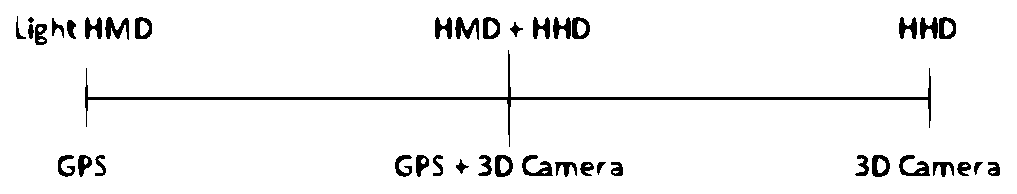
\includegraphics[width=.8\linewidth]{images/mgia16/tango_paper_continuum}
  \caption{The spectrum of AR tag tracking. A head-mounted display with GPS is ideal for outdoor tracking. Hand-held devices (3D camera) can be used for indoor tracking. Glass+Tango enables indoor AR tag tracking on light HMD.}
  \label{fig:mgia16:spectrum}
\end{figure}

\subsection{Implementation}


\begin{figure*}[t]
  \centering
  \includegraphics[width=\linewidth]{images/mgia16/workflow_diagram}
  \caption{System workflow.}
  \label{framework}
\end{figure*}


The system consists of two wearable devices a Google Glass HMD and a Google Tango chest-mounted 3D depth and sensor (see Figure\ref{framework}).

The two devices communicate with each other wirelessly. The Tango extends Glass' sensing ability by sharing the location and pose of the user as well as the tagged target position in the real world. The Glass dynamically overlays virtual tags based on the spatial information received from the Tango, and the background of the Glass display is set to black to act as an optical see through display (see Figure\ref{fig:mgia16:ui}). A white square is displayed on the Glass screen to indicate the center point at which the tango depth camera is facing. The user can initiate the wireless connection by using a three-finger touch gesture on the Glass touchpad, and the AllJoyn library  is used for networking.

Once the system starts on the Tango, it creates a reference coordinate of the surrounding environment. When the user moves, the motion sensor on the Tango will detect the body  position and rotation from the reference origin, both of which are then wirelessly transmitted to the Glass. Combing the head rotation detected by the sensors on the Glass, we can calculate the AR Viewpoint. The position of the AR viewpoint is calculated by adding a measured distance in height from Tango's position to adjust the height difference between the Glass and Tango. The orientation of the AR viewpoint mainly depends on the body's rotation but will be adjusted with the head and body pose difference, if the user turns their head towards a different direction from their chest. 

A speech recognition service is running in the background on the Glass to detect the users' voice input and convert it into text. The text will appear on the upper left corner of the display for for the users confirmation. This function is implemented as an Android service that utilizes Google API for speech recognition and so requires an internet connection. Once the user is satisfied with the recognized text, they can tap on the Glass touchpad while looking where they wish to add the AR tag by using the white square in the display. The Glass sends a request to Tango to identify the location of the AR tag in 3D space.

Combining the AR view point and the recognized text, we can convert the target position (the center point of the depth image indicated by the white square) to the global position relative to the origin. The Tango returns the global position of the AR tag to the Glass. This information is used to construct an AR tag with the speech recognized text that is overlaid on the top of the Glass camera view.

In (Figure\ref{fig:mgia16:ui}), the top left corner shows the last words captured via the voice recognition service, and a white square indicates the center position of Tango's RGB depth frame. The text in the middle of the display "Cup" is an AR tag overlaid on top of a physical cup. 
% * <eng.ala@gmail.com> 2015-06-19T10:04:56.888Z:
%
%  [Somewhere it would be good to mention the tracking accuracy and update speed – how accurate is the Tango position sensing for example]
%

\begin{figure}[ht]
  \centering
  \includegraphics[width=2.5in]{images/mgia16/WIN_20150614_204531_2}
  \caption{View through Glass display of a cup overlaid by an AR tag.}
  \label{fig:mgia16:ui}
\end{figure}


\subsection{User Study }

To evaluate our prototype, we conducted a pilot user study (see Figure\ref{fig:mgia16:scenario}) with ten participants . 4 female, 6 male ranging in age between 23 to 33 years old (\textit{SD= 4.35}). The main focus of the study was to measure the usefulness of the proposed system. Participants were asked to create three different AR tags for three different objects inside the room, with voice input, and then to walk around to observe how well the AR annotation is placed at the selected location. Participants had the freedom to assign any text to any object they wish in the test. The experiment conductor explained the tasks before the experiment and gave examples of target objects and names to use for voice input. All participants completed the tasks within 5 minutes. 

\begin{figure}[ht]
  \centering
  \includegraphics[width=3in]{images/mgia16/axis_lo}
  \caption{User study scenario}
  \label{fig:mgia16:scenario}
\end{figure}

Qualitative feedback about the system was collected from participants including how they would describe their experience using our system, what they liked and didn't like. Questions (Table \ref{table:questions}) were in four categories: (C1) Using the voice commands to create AR tag, (C2) Tap on glass touch panel to attach the AR tag, (C3)  Walk around to find AR tag stick to the original position, (C4) Overall AR tagging experience. In each category we asked the participants the following questions

\begin{table}[ht]
  \centering
	\caption{Survey questions}
    \label{table:questions}
    \begin{tabular}{r l}
    \hline
    Q1 & I found it easy to use \\ \hline
    Q2 & I found it natural to use \\ \hline
    Q3 & I found it physically challenging \\ \hline
    Q4 & I found it mentally challenging \\ \hline
    Q5 & I found it useful \\ \hline
    \end{tabular}
\end{table}

The answers were captured on a Likert scale of 1 to 7 in which 1 is "strongly disagree" and 7 is "strongly agree".

We used the Wilcoxon Signed Rank test on the results to measure significance. Based on the results, we found that participants rated significantly higher than neutral (4) on Q3 (p=.01, .009, .007 and .041) and Q4 (p=.014, .009, .007 and .01) for all categories (C1, C2, C3, C4). Q2 (p=.033) and Q5 (p=.015) were rated significantly higher for category (C3). Q1 for C4 was rated significantly higher (p=.014). (see \ref{survey_results}). The results  for other tasks were rated less significant than neutral level (4). Participants rated the task of walking around the environment was useful with average score of 5.2 out of 7 as well as being not mentally challenging with an average score of 2 out of 7. This highlights the usefulness of the system in assigning AR tags and recognizing them when they appear on their display while walking around the environment. 

In addition to the survey, we also asked participants open questions to comment on the system usability. A total of 3 out of 5 participants mentioned that they would use this system for virtual sticky notes, and they also provided some positive feedback such as "the system could be useful for finding a meeting room or a colleague's desk in an open plan area". There were also a few suggestions for improving the system, such as "allow the user to manually adjust the location of the AR tag" or "integrate with eye tracking to assist placing the AR tag within the field of view ". Participants appreciated  the concept of wirelessly connecting depth camera to a wearable HMD to enable the 3D spatial tracking.    


\begin{figure}[ht]
  \centering
  \includegraphics[width=\linewidth]{images/mgia16/user_study_results2}
  \caption{Average results of survey questions. Bars indicate standard error. *=statistically significant}
	\label{survey_results}
\end{figure}


\subsection{Discussion}

% * <eng.ala@gmail.com> 2015-06-19T10:05:25.941Z:
%
%  It would be good to add some more comments about why you got the results that you did
%
While our prototype  system demonstrates the concept of harmonizing the use of multiple wearable devices for AR visualization, there are few limitations in the current implementation of the system. It was observed that some users had difficulties with voice input as they were not native English speakers, which made the participants use several attempts before the intended word was correctly recognized.  

The current system tracks the 3D environment relative to the starting position, which requires the users to start the system at the same position and orientation in each test trail to keep the annotation in place between uses for sharing. This could be overcome in the future by storing the reconstructed 3D map of the environment and reusing it instead of generating it from scratch every time. 

\subsection{Future Application Scenarios}

Many implementation scenarios could benefit from combining a light head-mounted display with a chest worn 3D depth camera,  such as 1) Navigation, 2) Remote collaboration and 3) Social sharing. In this section we describe each of these in more detail.

Navigation is a scenario where this system can be useful. The user could navigate in an outdoor environment using GPS on Glass or similar smart glass display. Google Glass, being an unobtrusive head-mounted display, allows for hands-free navigation. However when the user enters a building, the GPS stops working and the system switches to indoor navigation using the 3D depth camera of the Google Tango device. Combining two devices enables seamless transition during a navigation experience. For example, a person could be shopping to find a particular item and use outdoor GPS tracking to guide them to the store. Once inside the store the Tango depth sensing hardware can help with navigating to find the particular product on the shelf.

Remote collaboration is another scenario where this application could be useful. A local user could transmit reconstructed 3D geometry of the environment using the Tango device to the remote user. The remote user will then have a more detailed view of the environment comparing to 2D sharing such as with a video stream. With the 3D geometry of the environment, the remote user can view the scene from different angles that helps provide better understanding of the surroundings of the local user. Placing AR tags in a 3D environment helps maintain the location of the AR tag especially when the viewing perspective is changed to the point from when it was original recorded

An additional use of the system could be in a social sharing experience where multiple users of the system could collaborate to add, edit and manipulate AR tags in the shared environment. 
% * <eng.ala@gmail.com> 2015-06-19T10:02:27.344Z:
%
%  put more information
%

\subsection{Summary}

This section presented a wearable AR system combining tracking technologies to provide a compelling indoor AR experience for spatial annotation application. By wearing the system, users can create virtual tags with text content generated by voice input and place it where they are looking at. The virtual tags can be visualized in place as a reminder for the users.  

Different scenarios can be implemented and tested based on the prototype with multi wearable devices. There are also a number of ways this research could be extended. In the future, we would like to further develop our efforts in designing interaction scenarios for our system, such as wearable gaming or collaboration. We also plan to develop the system further to expand the use of chest worn device for various interaction techniques (e.g. gesture recognition).


\input{Chapters/43-pano}


\chapter{Social Data in AR} % Main chapter title
\label{ch:data} % Change X to a consecutive number; for referencing this chapter elsewhere, use \ref{ChapterX}

This chapter addresses the surrounding environment of the user in terms of the social AR continuum. The surrounding environment level of detail can be determined based on the relationship between the user and the social contact with whom they are sharing the environment. The aim of this chapter is to answer the research question \ref{rq:interaction}: \textit{What is the best way to view and interact with shared social data on wearable AR displays?}. In this chapter we study two different ways of sharing the surround environment (360 Panoramas \ref{sec:surrounding:360}, 3D scanned surroundings \ref{sec:surrounding:environment}). We also look into partially sharing/hiding \ref{sec:surrounding:hiding} part of the environment with social contacts, based on privacy concerns. For each way of sharing, we discuss the levels of detail that can be shared based on the user relationships. 

\section{Filtering Shared Social Data}
\label{sec:surrounding:360}

The social data describing the surrounding scene can described in different levels of detail. A different ways of describing a surrounding scene include: a 2D image, a panoramic image, a video, a 360-degrees video, a 3D depth image, or a VR 3D model. These different ways of describing the same scene represent the levels of details that can be varied based on the Social AR Continuum and the social proximity between the social contacts. 

This section describes a method and a prototype implementation for filtering shared social data (e.g., 360-degree videos) using wearable AR devices (e.g., HoloLens) \cite{Nassani2018a}. The data filtering is based on the sharer-viewer relationships in order to preserve privacy. For example, when sharing a 360-degrees video, if the user has an intimate relationship with the viewer, then the full fidelity (i.e., the whole 360-degree video) of the user's environment is visible. However, if the two are strangers, then only a snapshot image is shared, and the user cannot get more information about the sharer's environment. By varying the fidelity of the shared content, the viewer can focus more on the data shared by their close relations and differentiate this from other content. Also, the approach enables the sharing-user to have more control over the fidelity of the content shared with their contacts for privacy.

% In this work, we are trying to answer the question, what would be the best way to share rich data (such as 360 videos) within a large social network? The hypothesis is that filtering data based on the user-viewer relationship or proximity will increase the feeling of being together or inter-connectedness. 


% =============================================================================
\subsection{Sharing Social Data}
% =============================================================================

From the perspective of the person who is sharing the data (the sharer) with their social contacts (Figure \ref{fig:data:sharer}), the data is collected in its highest fidelity (e.g., a fully spherical 360-degree view) which will be shared with those viewers with the closest (most intimate) social relationships. For less-intimate friends, a 2D video, extracted from the 360 videos based on the sharer's view direction over time, will be shared. For Strangers, the sharer can select which snapshot image from the 2D video sequence to display. The central metaphor is that the closer the relationship that the user has to the viewer, the richer data that they can share from their point of view (360-degree videos, 2D videos, still images).

\begin{figure}[ht]
    \centering
    \includegraphics[width=1.5in]{images/chi/images-04.eps}
    \caption{Sharing point of view with different fidelity of representation.}
    \label{fig:data:sharer}
\end{figure}

An example use-case scenario for filtering by sharer is where the sharer is going on a hike and wanting to share the experience of being in an interesting place such as near a river. The sharer takes a live 360-degree video of the surrounding environment and shares it with her followers. The sharer then gets to see how the followers are able to see the shared data based on their social relationship to her. The sharer's intimate friends and family will see the live 360-degree video, other friends the 2D video, and strangers still images of the scene, all automatically created from the 360-degree video recording.

% =============================================================================
\subsection{Viewing Shared Social Data}
% =============================================================================

The user viewing the shared data (the viewer) uses a wearable AR interface to see content from their social network superimposed over the real world, based on proxemics. For example, the viewer may be interested in seeing what their social contacts (followers) are up to and the places they have been. In this scenario the viewer can look around through the AR display to see their social contacts placed around them in three circles ordered by relationship. On top of each social contact, the viewer can see the content they are sharing, filtered based on the social relationship between the social contact and the viewer.

Based on our earlier work \cite{Nassani2017a}, the people who are socially closer will appear in the AR view visually closer and have a more realistic representation. The content shared by each social contact will appear above their avatar (see Figure \ref{fig:data:viewer}), and to view the content more clearly, the user can select it (e.g., using the HoloLens air-tap gesture) to bring the content closer or walk to move inside the 360-degree video sphere. The user can then tap again to bring back the content to its original place to see other social contacts. 

\begin{figure}[ht]
    \centering
    \includegraphics[width=3in]{images/chi/3_levels_of_data.png}
    \caption{Social contact sharing in different relationships with the viewer (Left to right: Intimate, Friend, Stranger). The shared data content (above the avatar) is filtered (360-degree video, 2D video, 2D image) based on social relationship.}
      \label{fig:data:viewer}
\end{figure}

In addition to this operation, this section proposes that the viewers can also see the shared content in different fidelity (360-degree videos, 2D videos or images) based on the social relationship with the sharer (Intimate, Friend or Stranger). While the sharer could restrict the fidelity of the shared content based on the social relationship as mentioned earlier, the viewer could also filter the content based on their preference. In order to avoid getting mentally overloaded by seeing too much content in high fidelity, the viewer should be able to choose the preferred fidelity for the shared content from each social contact. This could be achieved either explicitly by choosing a fidelity for each social contact, or implicitly by moving closer to or further from the avatar representing the contact.      

% =============================================================================
\subsection{Prototype}
% =============================================================================

To explore using the Social AR Continuum metaphor for sharing data between social contacts, a prototype was built using the Microsoft HoloLens. The prototype software was built using Unity 3D game engine, and it allows users to view their social contacts on a wearable AR interface. Figure \ref{fig:data:system} shows the structure of the prototype system. 

\begin{figure}[ht]
    \centering
    \includegraphics[width=3in]{images/chi/images-03.eps}
    \caption{System components.}
    \label{fig:data:system}
\end{figure}

The prototype places social contacts around the user (viewer) in three concentric circles which are controlled by the \textit{Circles Manager}. The social contacts have different visual fidelity and proximity based on their initial relationship to the viewer, and are rendered using the \textit{Avatar Controller}. The avatars were randomly pre-generated without any resemblance to actual contacts. MakeHuman\footnote{http://www.makehuman.org/} was used to generate the 3D avatars. The viewer (HoloLens user) can turn their head to face different social contacts and then use gestures (air taps) to interact with the contact (view their data or change their position which represents the social relationship). The interactions with HoloLens are enabled using the open-source library \textit{HoloToolkit}\footnote{https://github.com/Microsoft/MixedRealityToolkit-Unity}. The data content shared by the social contacts are controlled by the \textit{Data Controller} which determines which fidelity needs to be displayed based on the social relationship between the avatar and the viewer. The top-level \textit{Scenario Manager} defines the implementation needed for different conditions in the user study, including interaction with avatars, shared data and the concentric circles. 

% =============================================================================
\subsection{User Study}
% =============================================================================

A user study was conducted to test the system usability and effects on social presence, comparing the following conditions: 

\begin{itemize}
    \item C1) Baseline: Shows the shared 360-degree videos from all social contacts.
    \item C2) Tap-to-change: Filters the fidelity of the shared 360-degree videos based on the relationship between the viewer and the social contact. The user can tap on any social contact to cycle through different relationships.
    \item C3) Walk-to-change: Filter the fidelity of the shared 360-degree videos based on the physical distance between the viewer and the social contact.
\end{itemize}

The task was for participants to wear the headset and observe 12 social contacts (mocked up, not reflecting the participant's real social contacts) placed around the user at equal angles from each other to complete a circle (360 degrees) around the viewer, and at different distances to the viewer (centre) based on the social relationship. Each social contact had shared content floating above their head, filtered depending on the type of social relationship that the social contact had with the viewer. 

The participant could view the data content by performing the air-tap gesture on it. Once tapped, the content moved closer to the viewer. For instance, if the viewer tapped on the sphere of a 360-degree video, then the sphere immersed the participant to experience it, while for a 2D video, it was moved closer to the user so they could see it at full-screen resolution.

Participants were asked to answer the 5-point Likert-scale questions shown in Table \ref{tbl:questions} which are based on prior work \cite{Biocca2003}. Participants were asked to rate their experience on the Subjective Mental Effort Questionnaire (SMEQ) \cite{Sauro2009}. 

\begin{figure}[ht]
    \centering
    \includegraphics[width=1.5in]{images/chi/images-02.eps}
    \caption{Questionnaires for Social Presence including the following dimensions: CoPresence (CoP), Attentional Allocation (Atn), Perceived Message Understanding (MsgU). *=negative} 
      \label{tbl:questions}
\end{figure}

% =============================================================================
\subsection{Results}
% =============================================================================

A user study was run with eight participants (four female) aged 26-35 (SD=3.03). All participants used social networking platforms on a regular basis, and most (How many?) were familiar with AR/VR displays. 

After filling in a demographic questionnaire, the participants were asked to experience the three conditions in random order. Then they filled in a social presence questionnaire and SMEQ about the condition they just tried. After finishing all three conditions, participants then filled in a post-experiment questionnaire where they were asked about the overall experience and if they had any suggestions to improve it. 

From the questionnaire results (Figure \ref{fig:data:results}), indicates that C2 was rated (3.6) better in terms of social presence compared to C1 (3.3) on average, while C3 (3.5) was relatively close compared to C2. The SMEQ results show that all three conditions were rated low in terms of mental effort, while both C2 (M=16.875) and C3 (M=16.875) were rated lower than C1 (M=21).

\begin{figure}[h]
  \centering
  \includegraphics[width=\columnwidth]{images/chi/images-01.eps}
  \caption{Results of social presence (top) and SMEQ (bottom). *=reversed rating scale. Whiskers=standard error}
  \label{fig:data:results}
\end{figure}

As part of the post-questionnaire, participants were asked to rate the three conditions (1=least preferred, 3=most preferred). The ranking results (see Figure \ref{fig:data:ranking}) show that C1 was least preferred (1.3) while C2 (2.25) and C3 (2.375) were similar. There was a statistically significant difference in ranking conditions $\chi^2(2)=7, p=0.05$. A post-hoc analysis with Wilcoxon signed-rank tests was conducted, finding a statistically significant difference between C1-baseline and C3-Walk to change. ($Z=-2.081, p=0.037$), and no difference between the other conditions.

\begin{figure}[h]
  \centering
  \includegraphics[width=1.5in]{images/chi/images-05.eps}
  \caption{Condition ranking results. Reverse rating scale: 1=least preferred, 3=most preferred. Whiskers=standard error. $*=$ statistically significant difference (Friedman test: $X^2(2)=7, p<0.05$).}  
      \label{fig:data:ranking}
\end{figure}

% =============================================================================
\subsection{Discussion}
% =============================================================================

From a semi-structured interview after the experiment, most users found that condition C3 (walk to change) was a more fun and natural way to view shared data from social contacts. "I feel it is more real and fun to view the 360 videos by walking toward the avatar". Also, other subjects found that the walking condition was more suitable for an outdoor or open area to avoid running into obstacles while walking. The condition C2 (tap to change) was found more convenient for changing the relationship rather than requiring more physical effort, such as walking. The Baseline condition (C1) was the least favourite for participants, as it was too overwhelming having all 360-degree videos shown all around. 

On the downside, participants mentioned some weakness for condition C2 (tap to change), such as potential clutter by being able to bring all social contacts into a small area of the intimate circle. While condition C3 (walk to change) did not have that issue, it was mentioned that by walking one might accidentally change the relationship with other social contacts that the user was not focusing on. For example, the avatars behind or on either side of the user would be affected by user movement, even if the user did not intend to get close to them. Viewing 360-degree videos through an optical see-through display was considered not as ideal, as the 360-degree videos appear to be semi-transparent on top of the real environment.

Overall, participants expressed their interest in using such a system to manage and view their social contacts and shared content in AR, and that it would be useful and easy to use. 

% =============================================================================
\subsection{Limitations and Future Work}
% =============================================================================

This prototype used asynchronous sharing, where social contacts were not online at the same time, sharing live data; the shared content was previously prepared, and the 360-degree videos were previously processed to extract 2D video and a 2D image. However, the method was applied for filtering could be applied to synchronous sharing as well. In the future, the plan is to add live video streaming from social contacts and live scaling down of the content based on social relationships. 

% The concept does apply to synchronous sharing where social contacts are online at the same time. Future plans includes extending this prototype for synchronous sharing experiences. We can expand the implementation to include spatial audio as a fidelity option on which to filter based on social relationship. 

% Additionally, we will conduct a full quantitative and qualitative user study to measure the effects of filtering content type on social presence and user experience. 

% =============================================================================
\subsection{Conclusions}
% =============================================================================

This section presented a mechanism for presenting shared data content by filtering the content type based on the social relationships between the user and the social contacts. 

This work includ an implementation on HoloLens prototype for applying the proposed method in an asynchronous collaboration scenario and conducted a user study using the prototype. The study compared three conditions: viewing 360-degree video without filtering, filtering based on the social relationship, and filtering based on distance.

Initial results showed a trend of participants favouring having the option to filter data over not filtering. The results included a qualitative feedback that provides insights for future directions. 

\section{Filtering 3D Shared Surrounding Environments}
\label{sec:surrounding:environment}

In this work \cite{Nassani2018b}, we explore the social sharing of surrounding environments on wearable AR devices. In particular, we propose filtering the level of detail of sharing the surrounding environment based on the social proximity between the viewer and the sharer. We test the effect of having the filter (varying the levels of detail) on the shared surrounding environment, to preserve the sense of privacy from both viewer and sharer perspectives, and conducted a study using the HoloLens. We report on semi-structured questionnaire results and suggest future directions in the social sharing of surrounding environments.

This work explores new ways of sharing the remote environment of social contacts in a wearable AR interface. We build on top of our previous work \cite{Nassani2018a} that looked into sharing surrounding environments based on social proximity. Previously, we tested three levels of representing surrounding environments: 360-degree video, 2d Video and 2D Image. This work focuses on sharing 3D captured rooms and levels of detail that can be used based on social proximity. The significance of the work is that it addresses the privacy concerns of the sharer as well as the efficiency of placing the surrounding AR space of the viewer.

\subsection{Prototype System}

When the user puts on the HoloLens, he/she sees an AR user interface (UI) showing simulated social contacts (see Figure~\ref{fig:environment:setup}). The UI displays the social contacts around the viewer. Above each social contact avatar, the viewer can see a representation of the shared remote surrounding environment. The level of detail of the shared surrounding environment is determined by the social proximity to the viewer.

The user can air-tap on the environment above an avatar to expand it to life-size around the avatar (Figure~\ref{fig:environment:environment-levels}). The user can walk inside and explore the shared surrounding environment.

\begin{figure*}
    \centering
    \includegraphics[width=\columnwidth]{images/ismar18/images-06.eps}
    \caption{The viewer uses the HoloLens to view social contacts and proximity-filtered shared environments.}
    \label{fig:environment:setup}
\end{figure*}

\begin{figure}[ht]
  \centering
  \includegraphics[width=2in]{images/ismar18/images-05.eps}
  \caption{Levels of detail of the shared surrounding environment. 1) full details for Intimate contact: including family picture, bank balance and computer monitor. 2) partial details for Friend contact: hiding the family picture, bank balance, but keeping work-related items such as computer monitor. 3) limited details for Stranger contact: hidden personal and work related items.}
  \label{fig:environment:environment-levels}
\end{figure}

\begin{figure}[t]
  \centering
  \includegraphics[width=\columnwidth]{images/ismar18/images-04.eps}
  \caption{Top: the average results of subjective comfort questions. Middle: the percentage results of ranking the best condition. Bottom: the percentage results of voting for the best method to hide part of the environment. Whiskers indicate the standard error.}
  \label{fig:environment:results}
\end{figure}


The prototype was built using the Microsoft HoloLens\footnote{https://www.microsoft.com/en-us/hololens} and the Mixed Reality Toolkit\footnote{https://github.com/Microsoft/MixedRealityToolkit-Unity}. The avatars representing the social contacts were generated using MakeHuman\footnote{http://www.makehumancommunity.org/}. The 3D representation of the remote sharer's room was modelled in AutoDesk Maya\footnote{https://www.autodesk.com/products/maya/overview} to simulate 3D scanning of the user's surrounding environment. To test if users preferred to have a proximity filter applied on the shared surrounding environment, the prototype offers to turn the filter on or off in two conditions; a base-line (C1: no-filter) and a proximity filter applied (C2: proximity-filter).


\subsection{User Study}

We collected feedback from 10 participants (five female) with an average age of 28.8 ($SD=3.65$). The participants tried demonstrations of the two conditions: C1 (no filter), where all social contacts are sharing the full view of their surrounding environments, and C2 (proximity filter), where the shared surrounding environments are filtered based on three levels of social proximity (Intimate, Friend and Stranger) mapped to the level of detail of the shared surrounding environment (Full, Partial and Limited). The order of the conditions was randomised based on a Latin square. 

For each condition, we asked participants to rate how comfortable they felt (on a five-point Likert scale) about the sharing environment from the perspective of a sharer (person sharing) and the viewer (the person viewing) of the surrounding environment. We also asked participants to rank which condition they preferred (and to state why) from both perspectives. Finally, we asked about which method of hiding sensitive items in the shared environment the user preferred by selecting an option from 1) remove/hide the item as if it did not exist, 2) block/overlay a black box on the item so it will be hidden, 3) blur out the item, 4) other. 

We ran a Wilcoxon signed-rank test on the subjective perceived comfort in terms of privacy. The test showed that having a proximity filter (C2) applied on the shared surrounding environment did elicit a statistically significant improvement in perceived comfort in terms of privacy for both sharers ($Z=-2.831$, $p=0.005$) and viewers ($Z=-2.588$, $p=0.01$). 

As for the ranking results, C2 (proximity filter) was preferred by both sharers (100\%) and viewers (70\%) over C1 (no filter). C1 (no filter) was ranked 30\% for viewers. In terms of the preferred way of hiding sensitive items in the shared environment, blurring sensitive items (60\%) was preferred followed by removing/hiding sensitive items as if they did not exist (40\%) and the lowest was overlay (10\%). 

In the open-ended questions, C1 (no filter) was reported stronger in terms of the curiosity for the viewer. "... would suit supervisors who are interested in knowing details about their social network", one participant mentioned. The most reported strength of C2 (proximity filter) was around privacy and the sense of being comfortable in sharing levels based on social proximity. 

Overall, the results confirm our hypothesis of the value of social proximity-based filtering for sharing the surrounding environment. An interesting observation is that the sharer perspective may be different from the viewer perspective in terms of privacy. 

% In the future, we will extend this work to explore live (synchronous) sharing with both avatars and real people. Also, we will look into the perspective of the sharer and how they can select which part of the room to share with which level of social proximity contact.

\subsection{Conclusions}

In this work, we explored implementing the social AR continuum on sharing surrounding spaces between social contacts. We ran a study to test the effects of applying a filter on levels of detail on how comfortable the participants were in terms of privacy. We found that most participants are more comfortable when the social filter was applied to their shared surrounding environment. 
\section{The Social Continuum of Sharing Surrounding Spaces in Wearable AR}

% \subsection{Abstract}

This paper describes a system and a user study for sharing social surrounding spaces on wearable Augmented Reality (AR) devices. Unlike sharing for collaborative purposes, we focus on sharing between social contacts. We extend the previous work of the Social AR Continuum by exploring how sharing the surrounding environment can vary based on the social proximity between social contacts. We built a prototype for sharing a 3D captured room on a HoloLens, which enables the user to display three levels of social relationships: intimate, friend and stranger and maps them to three levels of the surrounding environment. In a user study with the prototype, we focused on how socially connected participants felt, as well as on how they felt knowing that they were sharing more or fewer details of their surrounding environment with their social contacts. We found that all participant preferred having a social filter when sharing a view of their environment over having no filter. We discuss the research findings and outline future directions for research in sharing social surrounding spaces on wearable AR devices. 
 

% Wearable Augmented Reality (AR) devices are becoming more affordable, available and ubiquitous, so there is a need to understand design considerations for this new platform. Previous research has looked into using wearable AR headsets for collaborative use, for example in enhancing face to face \cite{Billinghurst2002} or remote collaboration \cite{gupta2016you}. The research presented here explores the use of AR headsets for social interaction and shared experiences. 

% Future social interactions with wearable AR can be extrapolated from current social network interactions where friends share content and interact with others' content on mobile platforms such as Facebook and Instagram. One trend with mobile social networks is live streaming of a view of a user’s surroundings. For example, Facebook live allows a person with a mobile phone to live stream to remote collaborators. Similarly, wearable AR systems have already been developed that enable people to share a view of their surroundings. For example, the Shared Sphere work of \cite{lee2017mixed} allows a user with a wearable AR display to live stream a 360 video of their surroundings to a remote collaborator. 

It is easy to imagine that in the future it will be possible for wearable AR systems to be used to capture and share a 3D view of the user's surroundings with hundreds or thousands of followers on a social network. However, before this becomes commonplace, many exciting research questions should be addressed. For example, would a person be comfortable with sharing a view of their real space with relative strangers? This work aims to explore how wearable AR systems could share a user’s surrounding room environment with social contacts and to measure how comfortable the sharer and the viewer would feel regarding privacy in different interface options. 

In the remainder of the paper, we first report on related work that is informing our research, then describe a prototype system we have developed mocking up potential interface options. In sections 4 and 5 we present the design of a user study with the prototype and in sections 6 and 7 the results of the study. Finally, we end the paper with a conclusion and discussion of areas for future research.


% \subsection{Background}

% Our work extends earlier work in representing users in Augmented and Virtual Reality (VR), social networking, and AR information filtering. Previous researchers have studied the concept of "personal space" and "social bubbles" as proxemic interactions between people in different places \cite{Sousa2016}. They used floor projections and hand-held devices to communicate the presence of remote people. They also established a "gradual engagement model for remote proxemics" based on distance from the user which consists of 1) personal, 2) engaged, 3) peripheral and 4) ambient.

% \cite{Jo2016} studied the influence on co-presence of the background environment (AR vs VR) and the fidelity of the avatar representation of the remote user (photo-realistic vs pre-built). They found that more realistic avatars had a positive impact on the feeling of co-presence between remote collaborators. \cite{Volante2016} also studied the impact of the visual appearance of avatars (realistic vs. stylized) on the inter-personal emotional response of participants. 

% \cite{Fuchs2014} studied telepresence via a scanned 3D environment to enable social connections with people and simulated face-to-face interactions. The remote person was scanned and reconstructed live in the local environment. They forecast that 3D telepresence is going to be more popular when technology is more capable. Similarly, some companies (such as High Fidelity and Itsme3D) are building social VR experiences in which users are represented as 3D virtual avatars.

% Although there has been considerable research into social representation in VR, there has been very little research in AR. There are some challenges with AR, such as finding the best locations to fit virtual avatars in the real world, so they do not interfere with physical objects or appear suspended in mid-air. However, a social AR application can also allow people to see their friends while doing other tasks; users do not have to switch to an immersive VR environment to see their social contacts.

% If AR is to be used to represent contacts in social networks, there could be a large number of contact to show. So our research could also benefit from earlier work on different ways of managing large amounts of information in AR interfaces. \cite{Julier2002} showed how environmental cues such as distance, and user context could be used to filter AR content into the most relevant information. View management techniques can be used to ensure that virtual objects can be easily seen in collaborative AR interfaces \cite{Hollerer2001}. Similarly, an image-based can be used to ensure AR information tags do not overlap in the AR view \cite{Grasset2012}. 

% In some mobile AR applications, the technology can be used to share a view of the user's world. For example, remote collaboration systems have been developed where a local worker with an AR display can share a live video view of their working space with a remote expert \cite{Billinghurst2002}, and the remote expert can provide visual feedback with AR graphical cues. However, most of these systems have just been developed for collaboration between small numbers of users, and not for more extensive social networks.

% Compared to this earlier research our work is novel because it considers how a wearable AR interface could be used to share views of a user’s surroundings with a vast social network with people of different relationships. When connected in this way, people may want to control the amount of information about their surroundings shared. For example, users who are close friends in a social network may be happy to share a view of their surroundings and have the remote user appear as an AR avatar in their real space, while those that are strangers may only prefer to have an audio connection and not show anything of their surroundings to preserve their privacy \cite{Oetzel2011}.

% We extend our previous research of the social AR continuum \cite{Nassani2017a} that describe parameters/dimensions that can be used for sharing social experiences. Previously, we investigated visual representation of virtual avatars on social AR in \cite{Nassani2017b} where we filter representing social contacts (intimate, friend, acquaintance and stranger) based on social proximity. We also looked into filtering social data (360 video, 2D video and 2D image) in \cite{Nassani2018a} as well as filtering the surrounding environment (full, half and limited room) in \cite{Nassani2018b} based on social proximity. In this work (Figure \ref{fig:frontier18:social-filter}), we focus the feeling of privacy when sharing and viewing surrounding spaces as well as the hiding mechanism preferred by users. 

\begin{figure}
\begin{center}
\includegraphics[width=\linewidth]{images/frontier18/images-02.png}
\caption{Social filter applied to the shared room. a) In an Intimate relationship, everything is shared. b) For a Friend relationship, some sensitive items are hidden (e.g., family photo, stock market). c) While for a Stranger relationship almost everything is hidden in the room.}\label{fig:frontier18:social-filter}
\end{center}
\end{figure}

\subsection{System}


We built an AR prototype system on the Microsoft HoloLens\footnote{https://www.microsoft.com/en-us/hololens} that connects a person (the sharer) sharing a view of their surrounding physical space to a remote person (the viewer) viewing the shared virtual room overlaid on top of their physical space. Figure \ref{fig:frontier18:system} shows the components of the system that we developed.

In the future, it will be possible to scan and immediately create a 3D model of the wearable AR user’s surroundings. However, we emulate this by creating a virtual 3D room modelled to match the sharer’s real room as if has been 3D scanned (see figure 2).  The 3D modelling was done on Autodesk Maya\footnote{https://www.autodesk.com/education/free-software/maya} and rendered on the HoloLens display using the Unity3D\footnote{https://unity3d.com/} game engine. The avatars representing the remote people are generated using MakeHuman\footnote{http://www.makehumancommunity.org/}.

We used UNET\footnote{https://docs.unity3d.com/Manual/UNet.html} as the high-level networking API from Unity to synchronise the state of the shared room and the remote person. The state of the remote person includes 1) the position and rotation of the virtual avatar representing the remote person, 2) the level of detail of the avatar based on the social relationship (i.e., stranger=half 2D image, friend=2D image, intimate=3D avatar). The synchronised state of the room involves changing the level of detail of the shared room depending on the social relationship as well as which part of the room is hidden by the user. 

\begin{figure}
\begin{center}
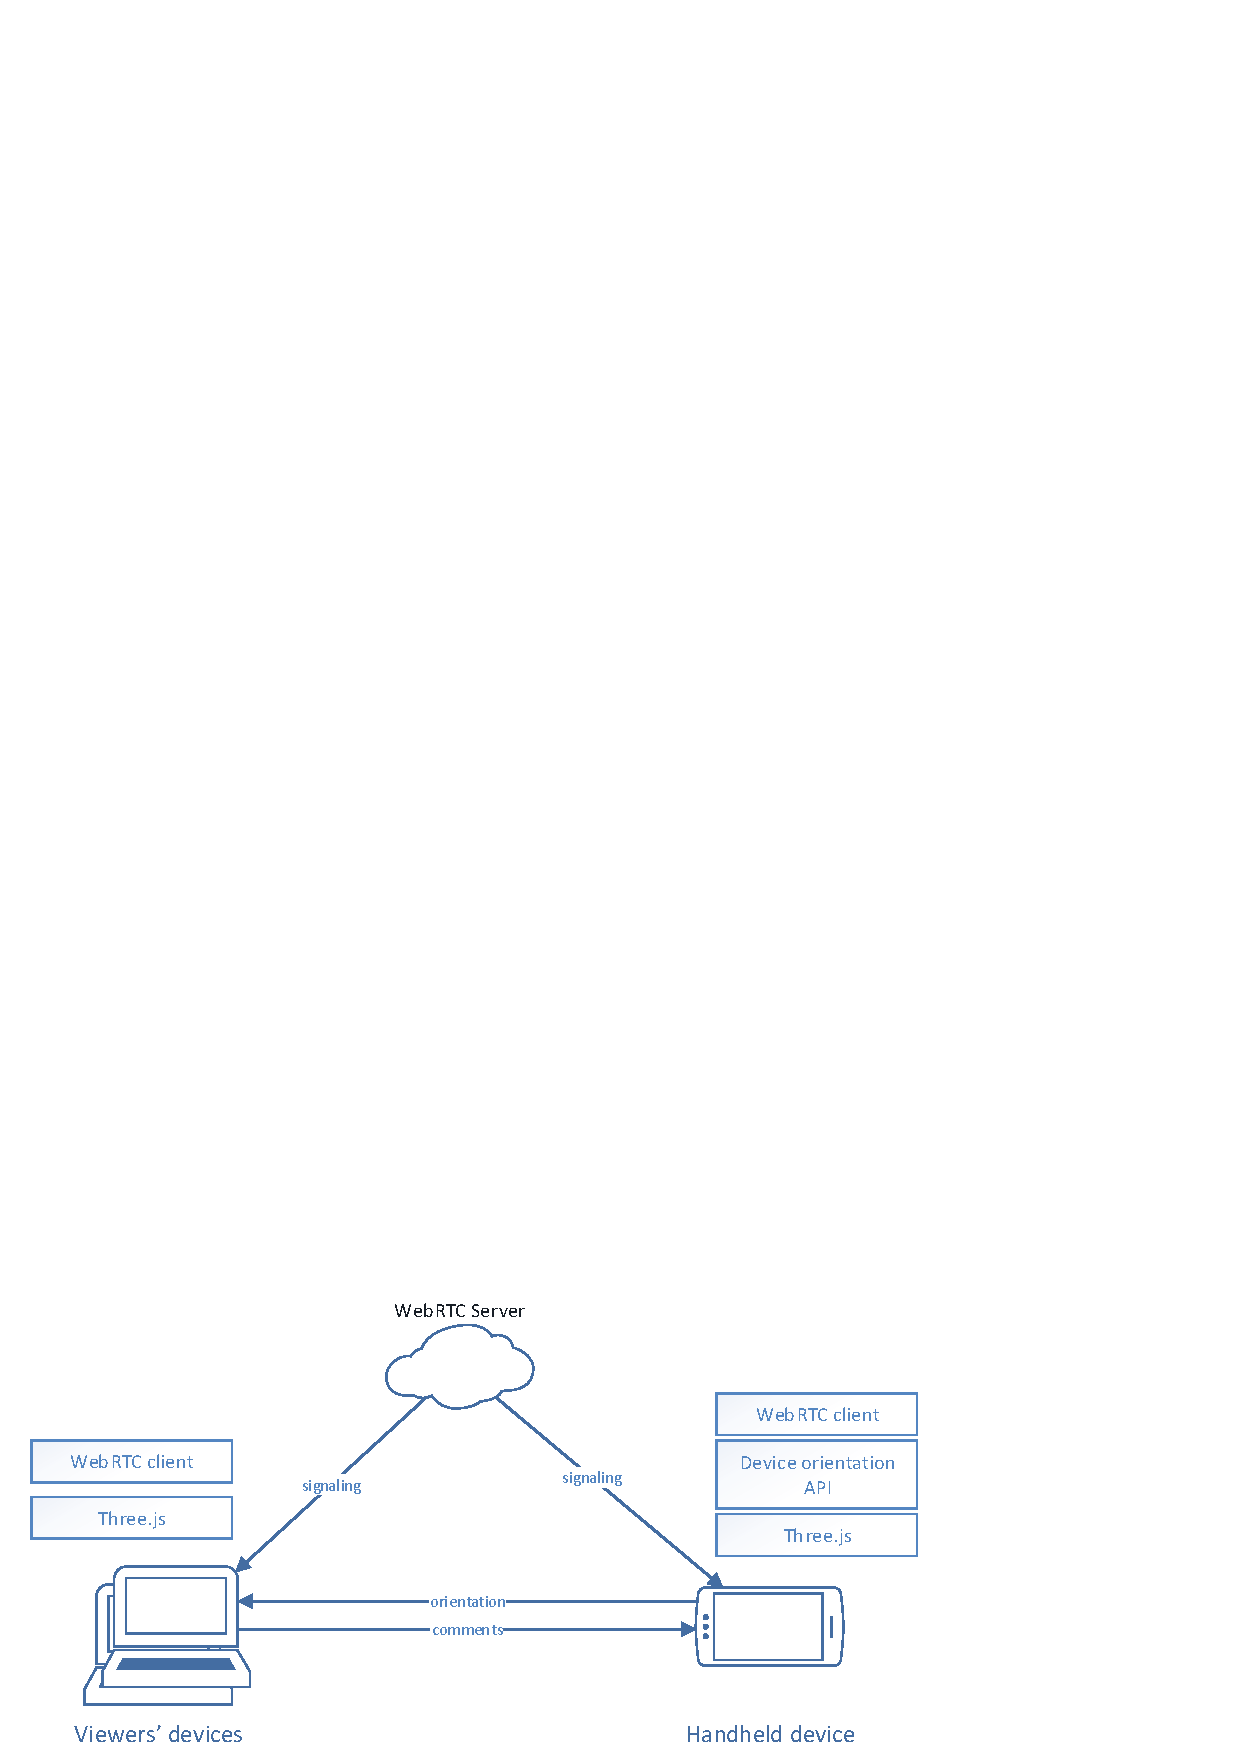
\includegraphics[width=\linewidth]{images/frontier18/system.jpg}
\caption{System components representing the sharer server-side (left) sharing with the viewer client-side (right) via WiFi: 1) the avatar position and orientation, 2) the social relationship data and 3) room and hidden components data. The system is built on Unity and runs on HoloLens.}\label{fig:frontier18:system}
\end{center}
\end{figure}

\subsection{User Study}

Using the prototype system we wanted to explore sharing different views depending on the social relationship between users, and also different methods for maintaining privacy. To do this, we conducted a pilot user study, with 12 participants (4 female) aged (25 – 43, median=32, SD=4.96). 
We asked participants to do two tasks: 

Task 1: View/share a room with or without a social proximity filter (see Figure \ref{fig:frontier18:social-filter}). In this task we had two conditions: 

\begin{itemize}
\item T1C1: Shared room without a social proximity filter where the level of details of the shared room is not affected by the social relationship between the users.
\item T1C2: Shared room with a social proximity filter where the level of details of the shared room is changed based on the social relationship between the users. 
\end{itemize}

Task 2:  The mechanism of hiding room parts for social proximity filter (see Figure \ref{fig:frontier18:hiding-mechanism}). In this task we had three conditions:

\begin{itemize}
\item T2C1: Remove – where objects are hidden by being removed from the viewer’s scene.
\item T2C2: Overlay – where objects are hidden by being overlaid by a white box. 
\item T2C3: Blur – where objects are hidden by appearing blurred to the viewer. 
\end{itemize}

Each participant tried the conditions from both sides of a viewer and a sharer. We asked participants to rate their experience after each condition. At the end of each task, we asked them to compare the conditions to each other and rank them. 

\begin{figure}
\begin{center}
\includegraphics[width=\linewidth]{images/frontier18/images-01.png}
\caption{Hiding mechanism applied on the TV screen. a) Remove, b) Overlay, c) Blur.}\label{fig:frontier18:hiding-mechanism}
\end{center}
\end{figure}


% \subsection{Experiment}

Figure \ref{fig:frontier18:setup} shows that the experiment was set up in two similar rooms so that the sharer was sharing his/her room with a remote viewer. The relative position and rotation of each user were synchronised and represented as a virtual avatar in the remote person view. The sharer could change the social relationship with the viewer by using 3-buttons (intimate, friend, stranger) situated in the middle of the room. The viewer could request the relationship to change by clicking on one of the relationship buttons. Once this happens, the sharer saw the relationship request in a different colour, which then they could approve and change the social relationship

After completing each task, we asked participants (see Table \ref{tab:frontier18:questions}) to answer three sets of Likert questionnaires; six bi-polar questions (BP), six co-presence questions (CoP) and three subjective questions (S) to measure the sense of privacy.  

\begin{table}
    \centering
    \begin{tabular}{ll}
BP1 &    Impersonal-Personal\\
BP2 &    Cold-Warm\\
BP3 &    Colourless-Colourful\\
BP4 &    Unsociable-Sociable\\
BP5 &    Closed-Open\\
BP6 &    Passive-Active\\
CoP1    &   I noticed my partner\\
CoP2    &   My partner noticed me\\
CoP3    &   My partner's presence was obvious to me\\
CoP4    &   My presence was obvious to my partner\\
CoP5    &   My partner caught my attention \\
CoP6    &   I caught my partner's attention\\
S1  & Uncomfortable-Comfortable\\
S2  & Insecure-Secure\\
S3  & Not-Interested-Interested\\
    \end{tabular}
    \caption{Subjective questions we asked participants to rate their experience on a 7-point likert scale}
    \label{tab:frontier18:questions}
\end{table}

We asked the participants open-ended questions about the strength and weakness of each condition. We also asked them to rank from most preferred to least preferred condition for each task, then explain the reason for why the chose the best and the worst condition. 

\begin{figure}
\begin{center}
\includegraphics[width=\linewidth]{images/frontier18/experiment-setup.jpg}
\caption{Experiment setup. The sharer (right) is sharing his/her 3D room with the viewer (left). The viewer sees the virtual room of the sharer overlaid on top of her/his physical room. Each user is seeing the remote person as a virtual avatar in their environment that has the position and orientation mapped to remote person.}\label{fig:frontier18:setup}
\end{center}
\end{figure}

\subsection{Results}

Figure \ref{fig:frontier18:result-filter-viewer} shows the Likert scale results for the viewer, while Figure \ref{fig:frontier18:result-filter-sharer} shows the results for the sharer. A Wilcoxon signed-rank test on the results of Task1 comparing no social filter (T1C1) and social filter (T1C2) showed that as a viewer having a social filter (T1C2) did elicit a statistically significant difference in BP5-Open (Z = -2.323, p = 0.02) and CoP1-I noticed my partner (Z =-2.066, p = 0.039). While as a sharer, having a social filter (T1C2) did elicit a statistically significant difference in CoP3-My partner's presence was obvious to me (Z = -1.993, p = 0.046) and CoP5-My partner caught my attention (Z = -2.164, p = 0.030) and S1-Comfortable (Z = -2.503, p = 0.012) and S2-Secure (Z = -2.816, p = 0.004). There was no difference in reponse to the other questions.

A Wilcoxon signed-rank test on the results of Task1 comparing no social filter (T1C1) and social filter (T1C2) showed that as a viewer having a social filter (T1C2) did elicit a statistically significant difference in BP5-Open (Z = -2.323, p = 0.02) and CoP1-I noticed my partner (Z =-2.066, p = 0.039). While as a sharer, having a social filter (T1C2) did elicit a statistically significant difference in CoP3-My partner's presence was obvious to me (Z = -1.993, p = 0.046) and CoP5-My partner caught my attention (Z = -2.164, p = 0.030) and S1-Comfortable (Z = -2.503, p = 0.012) and S2-Secure (Z = -2.816, p = 0.004).

In response to the ranking questions (Figure \ref{fig:frontier18:result-ranking}), all 12 participants preferred having a social filter when sharing room over having no filter (i.e., showing everything in the room to all social relationships). As for ranking the hiding mechanism, the most preferred option for hiding sensitive data in the room was the Remove option followed by the Overlay option, while the least preferred option was Blurring. 
We also asked participants if there was a different mechanism of hiding objects in their shared room that they would prefer (such as replacing the hidden object with a similar but less sensitive one). About 42\% thought that replacing the object was a good idea; however, most of them raised concerns about how they may not like the additional effort needed for selecting a similar object to replace.

\subsection{Discussion and Future Work}

The ranking results show that having the social filter is preferred over no social filter. However, in Likert questions, we found statistical differences in 2-5 questions out of 15. Participants with the sharer point of view had a more statistical difference than those with the viewer point of view which indicates that having a social filter is essential for people to feel comfortable regarding privacy when they have to choose. However, not as much when they have to go through the efforts of selecting which objects to hide for each social relationship.  

In the future, we would like to allow users to customise their room so that they feel more attached to the space they are sharing. In this user study, the sharer was hiding objects in the room while the viewer was observing the shared room synchronously. In the future, we can study if hiding before the viewer is connected asynchronously would affect the sense of co-presence or the feeling of being comfortable with sharing. We also would also allow participants to choose their avatars from a predefined list rather than being assigned an avatar randomly.   

\subsection{Summary}

In this paper, we described a HoloLens prototype built to share a 3D surrounding environment with social contacts, and simulate a future wearable AR social networking application; which was designed to explore how users would be willing to share views of their surroundings with remote people with different social relationships. 

We allowed users to choose which part of the room to hide or show to different social groups (intimate, friends, strangers). We run a pilot user study to test the effect of using a social filter on co-presence and the feeling of privacy from both sides as a sharer and a viewer. We found that all participants preferred having a social filter, and there was some statistical difference regarding feelings of co-presence and privacy. 

\begin{figure}
\begin{center}
\includegraphics[width=.8\linewidth]{images/frontier18/images-03.eps}
\caption{Results of social filter as viewer. *= statistically significant}\label{fig:frontier18:result-filter-viewer}
\end{center}
\end{figure}

\begin{figure}
\begin{center}
\includegraphics[width=.8\linewidth]{images/frontier18/images-04.eps}
\caption{Results of social filter as sharer. *= statistically significant}\label{fig:frontier18:result-filter-sharer}
\end{center}
\end{figure}



\begin{figure}
\begin{center}
\includegraphics[width=.9\linewidth]{images/frontier18/images-05.eps}
\caption{Results of hiding mechanism as viewer.}\label{fig:frontier18:result-hiding-viewer}
\end{center}
\end{figure}

\begin{figure}
\begin{center}
\includegraphics[width=.9\linewidth]{images/frontier18/images-06.eps}
\caption{Results of hiding mechanism as sharer.}\label{fig:frontier18:result-hiding-sharer}
\end{center}
\end{figure}

\begin{figure}
\begin{center}
\includegraphics[width=.8\linewidth]{images/frontier18/images-07.eps}
\caption{Results of ranking conditions.}\label{fig:frontier18:result-ranking}
\end{center}
\end{figure}

\section{Summary}

This chapter explored different options of representing social data through wearable AR between social contacts. The explored options include: 1) the type of shared social data, 2) filter 

\todo[inline]{add more}


\chapter{Visualising Social Contacts} % Main chapter title
\label{ch:contacts} % Change X to a consecutive number; for referencing this chapter elsewhere, use \ref{ChapterX}

After studying the about the social interaction/annotation (Chapter~\ref{ch:annotation}) and sharing data (Chapter~\ref{ch:data}), this chapter focus on how to represent social contacts through a wearable AR device. The representation of social contact varies based on their relationship with the user. A user study is conducted to test different conditions on the visual fidelity and proximity dimensions. 


% =============== PREVIOUS WORK ================

% A. Nassani, G. Lee, M. Billinghurst, T. Langlotz, and R. W. Lindeman, “Using Visual and Spatial Cues to Represent Social Contacts in Wearable AR” in SIGGRAPH ASIA 2017 Mobile Graphics and Interactive Applications. 

% =============== PREVIOUS WORK ================



\section{Proximity and Visual Fidelity}

One of the key problems with representing social networks in Augmented Reality (AR) is how to differentiate between contacts. In this paper we explore how visual and spatial cues based on social relationships can be used to represent contacts in social AR applications, making it easier to distinguish between them. Previous implementations of social AR have been mostly focusing on location based visualization with no focus on the social relationship to the user. In contrast, we explore how to visualise social relationships in mobile AR environments using proximity and visual fidelity filters. We ran a focus group to explore different options for representing social contacts in a mobile an AR application. We also conducted a user study to test a head-worn AR prototype using proximity and visual fidelity filters. We found out that filtering social contacts on wearable AR is preferred and useful.  We discuss the results of focus group and the user study, and provide insights into directions for future work.

% Rob: The abstract should give the results/findings we found in summary.
%  You should summarise the main findings in the abstract.

\begin{figure}[ht]
  \includegraphics[width=\textwidth]{images/20170618_031128_HoloLens_cropped}
  \caption{Representing social contacts in AR with different levels of proximity and visual fidelity}
  \label{fig:contacts:overview}
\end{figure}



% \section{Introduction}

% With major industry players (e.g. Microsoft, Facebook and Apple) supporting Augmented Reality (AR), it is likely that one day people will soon be using head-worn AR displays on a daily basis. One potential use for this technology could be for connecting with social networks. Just as people today use their mobile phones to connect with hundreds or thousands of "friends", wearable AR displays could be used to connect with friends and view and interact with their shared information.

% Previously, handheld and wearable AR systems have been used to view social networks in a number of different ways. For example, Presslite's Twitter 360\footnote{https://www.youtube.com/watch?v=5w7EAz8-uwU} shows virtual tweets overlaid on the real world at the locations of the people that sent them, and early versions of Junaio\footnote{https://en.wikipedia.org/wiki/Junaio} allowed people to drop virtual messages and pictures in the real world, as did the popular application Sekai Camera\footnote{https://www.youtube.com/watch?v=oxnKOQkWwF8\&t=61s}. Most of these applications were focused on asynchronous collaboration, enabling people to post virtual messages in space which can later be browsed and retrieved by other users. However similar technology could also be used for live synchronous collaboration such as a live video streaming the remote user point of view \cite{Nassani2016}, live video avatar sharing  \cite{Billinghurst2002}, or sharing realistic 3D models superimposed over the real world \cite{Fanello2016}.

% or by using virtual avatars to show a live view of remote collaborators and their surrounding space as in the Holoportation system  \cite{Fanello2016} which shows a realistic 3D AR representation of a remote collaborator.

% Tobias: Make clear here that scrolling etc is no option as we are constrained by the interactions and would require unobtrusive interactions.
% Unlike for handheld devices, by using a wearable AR display like the Microsoft HoloLens\footnote{https://www.microsoft.com/en-nz/hololens}, it could be possible to see an AR representation of the user's social network visible at all times. However, this raise the question of how to visually represent the contacts in the network. For example, if a user has a large social network with hundreds of contacts available, visually representing each of themmight clutter the user's visual space.

In our research we are interested in how to represent a social network with hundreds or thousands of contacts in a wearable AR interface. If there are dozen of virtual tags in an AR view representing people, how can they be distinguished between each other? How will this scale to hundreds or thousands of people? This is an important area of research as it will allow users to view and interact with a large number of social network followers at different levels of privacy and social engagement.

% One  of the challenges we are seeking to address is how to manage and represent communication from dozens, hundreds or thousands of contacts in a social network in an AR interface. If there are dozens of virtual tags in view representing people on the user's social network, how can they be distinguished between each other? How will this scale to hundreds or thousands of people?

% \section{Related work}

% Our work extends earlier work in representing users in Augmented and Virtual Reality (VR), social networking, and AR information filtering. Previous researchers have studied the concept of "personal space" and "social bubbles" in terms of proxemic interactions between people in different places \cite{Sousa2016}. They used floor projections and hand-held devices to communicate the presence of remote people. They also established a "gradual engagement model for remote proxmics" based on distance from the user which consists of 1) personal, 2) engaged, 3) peripheral, and 4) ambient.


% Rob: It is not good practice to use a citation as a part of speech (in this case, the subject). It is better to refer to the researchers (or the system/technique name), then give the citation. For example, "Jo [Jo et al., 2016] studied..." You should correct this throughout the paper.

% Jo \textit{et al.} studied the influence on co-presence of the background environment (AR vs VR) and the fidelity of the avatar representation of the remote user (photo-realistic vs pre-built) \cite{Jo2016}. They found that more realistic avatars had a positive impact on the feeling of co-presence between remote collaborators. Volante also studied the impact of visual appearance of avatars (realistic vs. stylized) on inter-personal emotional response of participants \cite{Volante2016}. They also found that more visual realism has lower negative effects.

% Fuchs \textit{et al.} studied telepresence via scanned 3D environment to enable social connections with people, and simulated a face-to-face interactions \cite{Fuchs2014}. The remote person was scanned and reconstructed live to the local environment. Their forecast is that 3D telepresence is going to be more popular when technology is more capable.

% Researchers  have been investigating social aspects of multi-user VR environment. %\cite{Ducheneaut2006} studied massive multiplier online games in terms of social activities, and  found that while users may prefer to be with other players, they don't necessarily like actively interacting with them. This led us to thinking that users may want to have the sense of the presence of social contacts around them, but not necessarily interact with them.

% \cite{Harris2009} studied the social behaviour of users of Second Life, and they found that users become less active over time and go to familiar places rather than being explorative and actively teleporting/flying. This suggests that people prefer routine and to be surrounded by familiar faces/places over time, forming social group.

% Some companies (such as High Fidelity\footnote{https://highfidelity.com/} and Itsme3D\footnote{https://www.itsme3d.com/}) are building social VR experiences in which people are represented as 3D virtual avatars.
% mark: [you should about how they handle crowds or if everyone is just represented the same] 
% However, there has been very little research into social representation in AR. The AR space is more challenging in terms of finding the best locations to fit avatars in the real world so they don't interfere with physical objects or appear suspended in mid-air. However, a social  AR application can also allow people to see their friends while doing other tasks; users don't have into switch to an immersive VR environment to see their social contacts.

% Researchers have also explored different ways of managing a large amount of information tags in AR interfaces.  Julier et al. showed how environmental cues such as distance, and user context can be used to filter AR content into the most relevant information \cite{Julier2002}. Hollerer et al. describe how view management techniques can be used to ensure that virtual objects can be easily seen in collaborative AR interfaces \cite{Hollerer2001}. Similarly Grasset et al. show how an image-based approach can be used to ensure AR information tags don't overlap in handheld AR \cite{Grasset2012}. 

% Previous research has explored how to filter information tags in AR interfaces based on user preferences [ref] and [ref], or even automatically based on context [To et al. 2016]. 
% mark: [Add more here]

% This previous research shows that visual fidelity can be used to distinguish between virtual avatars. Different visual representations and spatial cues can also be used to distinguish between information tags in an AR interface. However there has been little or no research on how to manage social network representations in AR for large numbers of connections. In the next section, we show how visual and proximity cues could be used to organize contacts in a wearable social AR interface.

% Allowing users to view and interact with a large number of social contacts requires filtering and categorizing information.  One way to filter/categorize contacts could be to arrange them along a social continuum, depending on how close they are to the user. For example, grouping people into Intimate Family, Friends, Colleagues and Strangers (see table \ref{tbl:visual-fidelity-proximity}), or more categories. These categories could then be shown using different levels of visual fidelity and proximity, enabling the user to easily tell the difference between people in their social network.

% \begin{table}
% 	\centering
% 	\caption{Using Visual Fidelity and Proximity to Categorise Friends}
% 	\label{tbl:visual-fidelity-proximity}
% 	\begin{tabular}{|l|l|l|}
% 		\hline
% 		\textbf{Category} & \textbf{Visual Fidelity} & \textbf{Proximity}       \\ \hline
% 		Intimate          & 3D avatar 				 & \textless1m, same space  \\ \hline
% 		Close friend      & 2D avatar                & 1-5m, close              \\ \hline
%         Acquaintance      & Bust image			 & 5-20m, nearby            \\ \hline
% 		Stranger          & Emoji			         & \textgreater20m, distant \\ \hline
% 	\end{tabular}
% \end{table}


In terms of visual fidelity, the representations of people in each of these categories could be increasingly more realistic as the categories change from Stranger to Intimate Family 
% (see figure \ref{fig:contacts:visual-fidelity-continuum}). 
For example, a user may see their spouse as a realistic virtual human superimposed over the real world, but a distant acquaintance would be a simple icon.
% \begin{figure}[ht]
% 	\centering
% 	\includegraphics[width=3in]{images/writing-images-07.eps}
% 	\caption{Changing visual fidelity over social continuum}
% 	\label{fig:contacts:visual-fidelity-continuum}
% \end{figure}
In terms of proximity, previous studies have shown that the distance between people in social settings varies according to their level of closeness \cite{Anslow2016}. We can use this to place the virtual representations of people in the real world around the user. The people that are intimate family and friends could be shown as visually closer to the user, while people who are strangers would be shown further away (see figure \ref{fig:contacts:proximic-circles}). This could be done using a body-centric virtual information space that travels with the user when they move.

The combination of using visual fidelity and proximity to categorize people from a user's social network would make it significantly easier for them to pay attention to the people that they want to. For example close friends would be represented as life-like virtual avatars near to the user, and so easily distinguished from strangers that are emoji icons further away.

\begin{figure}[ht]
  \centering
  \includegraphics[width=3in]{images/writing-images-11.eps}
  \caption{Proxemic \& Visual Fidelity Filtering of Avatars}
	\label{fig:contacts:proximic-circles}
\end{figure}

% Mark: You could move this to the future work section in the conclusion
% Other cues could be explored as well, such as placing people closer to the centre of the visual field who are more important/active, using colour to distinguish which users are currently available, or providing spatial audio cues to guide a person's attention.


\subsection{Implementation}

Using the social continuum metaphor from the previous section, we developed a prototype on the HoloLens to represent a user's social contacts in an AR environment. 
The prototype was built using Unity3D\footnote{https://unity3d.com/} 5.6 and HoloToolkit-Unity\footnote{https://github.com/Microsoft/HoloToolkit-Unity}, and the 3D avatars are from Morph3D\footnote{https://www.morph3d.com/}. 

% shows an overview of the system components. The scenario manager control the condition of the experiment, while the Friends Manager controls how friends are rendered. The Circle manager controls initial placing of the circles around the user. Spatial mapping is used to place circles and social contacts on the floor. Morph3D is used for rendering 3D avatars.

The prototype (figure \ref{fig:contacts:system-diagram}) uses the HoloLens Spatial Mapping feature to place virtual concentric circles (Circle Manager) on the ground around the user's initial position. On these circles, the social contacts are represented (Friend Manager) by either: a generic person silhouette, a 3D avatar, a 2D image, a bust image, or an emoji. The Scenario Manager controls the application, while the Friends Manager controls how friends are rendered. The Circle Manager controls initial placing of the circles around the user. Spatial Mapping is used to place circles and social contacts on the floor. Figure 1 shows the AR view of the user's social network.


\begin{figure}[ht]
  \centering
  \includegraphics[width=3in]{images/system-diagram.eps}
  \caption{System components}
	\label{fig:contacts:system-diagram}
\end{figure}


% mark: It would be good to have a figure showing the AR interface

% mark: [It might be good to add more information here about the hololens interface – software used to build it in (Unity?) content used etc]

To arrange the social network, the user can use hands gestures (e.g. tap and drag) to move a virtual avatar closer or further away from the centre of the circles, changing the social group the contact belongs to, and the representation of the avatar automatically updates to match the selected social group. For instance, if the user selects a 3D avatar from the Intimate circle and moves her to the Friends circle, then her representation will turn into a bust image to reflect the destination social group.

% TODO: (Gun) Add some screen captures of the prototype implementation on HoloLens. Would be good to have the four conditions shown with this. Or is Figure 1 for this? Then you should better refer to the figure here in the text. Also would be nice to have the pictures to have a background of real environment to make it clear it is an AR visualization, rather than fully virtual.

% TODO: add system image + UI screenshot

\subsection{Focus Groups}

% Mark: You should say how many men and women there are and their ages.
To evaluate the interface concept and collect feedback from potential users, we conducted two focus group sessions with a total of 11 participants. 
The first group consisted of six post-graduate students working on AR/VR research. The second group was a mix of five professional visual graphics and user experience designers who have not worked on AR/VR before. 
Each session was divided into two activities: (1) user participatory design and (2) a usability test with the prototype. 

The focus group began with a discussion and brainstorming session on how to visualise social network contacts in an AR environment. We briefly introduced the concept of social networking in AR and the challenges observed including visual clutter, yet no demonstration of the prototype system was given to avoid priming.
This activity included three tasks: 
% \textit{Task 1}) Imagine the future of social networks in AR. \textit{Task 2}) Map social groups in terms of physical distance. \textit{Task 3}) Map social groups in terms of visual fidelity.

\begin{itemize}
	\item T1: Imagine the future of social networks in AR 
	\item T2: Map social groups in terms of physical distance 
	\item T3: Map social groups in terms of visual fidelity 
\end{itemize}


\textit{Task 1}: We asked participants to draw or describe their vision of the future of how to represent social networks in AR. They then presented their ideas to the group and exchanged feedback.

% TODO: (Gun) Any figures to show the task?

\textit{Task 2}: We asked participants to order four different social groups (Intimate, Friend, Acquaintance, Stranger) in terms of physical distance from the user. We gave them four silhouettes that had one of the social groups written on the top and asked them to place silhouettes on an arrow that has four position; closest, close, far and farthest.

\textit{Task 3}: We asked the participants to match four different types of visual fidelity (3D avatar, 2D image, Bust image, Emoji) to four social groups (Intimate, Friend, Acquaintance, Stranger). This task included two sets of avatars, one male and one female.

In the second session, the usability test, we gave a demonstration of the prototype implementation, and asked participants for feedback on the following four conditions (see Figure \ref{fig:contacts:conditions}): 

\begin{figure*}
	\centering
	\includegraphics[width=\linewidth]{images/conditions-transparent-background}
	\caption{Four conditions of representing social contacts as seen through HoloLens; Baseline (B): same distance and visual, Proximity (P): different distance, Visual Fidelity (V): different visual, and Combined (C): different distance and visual}
	\label{fig:contacts:conditions}
\end{figure*}


\textit{Baseline (B):} all avatars had the same visual representation (silhouette) and they were at the same distance away from the user.

\textit{Proximity (P):} the avatars were placed at different distances from the user based on their social intimacy (the Intimate group was the closest, then Friends, then Acquaintance, then Strangers). However, they were all a silhouette representation.

\textit{Visual Fidelity (F):} the avatars placed at the same distance but had different visual representations based on their social group. The Intimate group was represented by an animated 3D avatar that moved and looked around. Friends were represented by 2D static images. Acquaintances in 2D busts, and Strangers were emojis.

\textit{Combined (C):} used both proximity and visual fidelity to filter social connections based on their social group.

Each participant tried the four conditions in a random order and for each condition, participants filled out a System Usability Scale (SUS) questionnaire \cite{brooke1996sus}. They also answered the following three subjective questions, on a Likert scale of 1 to 7, where 1=\textit{Not very natural/easy} and 7=\textit{Very natural/easy}:

\begin{itemize}
	\item SQ1: How natural was the mapping of proximity to social relationship?
	\item SQ2: How natural was the mapping of visual fidelity to social relationship?
	\item SQ3: How easy was it to distinguish between the different avatar types?
\end{itemize}

\subsection{Results}

% mark: It would be good to talk about the two different groups – one from Uni and one from work.
We recruited 11 participants (four female, aged between 16 and 41 years old, Median=29, SD=5.89). Most (85\%) used social networks (e.g., Facebook, Instagram, Snapchat) on a daily basis, and about 60\% reported using AR/VR headsets (e.g., HoloLens, HTC Vive) on a monthly basis or more often. Only two people reported having no experience with AR/VR headsets before.

\subsection{User Participatory Design}

% The focus group consisted of three tasks in the brainstorming session: 

For \textit{task 1}, when asked about how would they imagine representing social contacts in an AR platform, there were the two main recurring themes, listed in the order of popularity.

\textit{Theme 1 - Virtual Avatars}: Display virtual avatars representing friends around the users using spatial cues to distinguish them. The user can interact with other avatars to see their interests, posts or their location. The user can initiate a voice or video call with one of their contacts by interacting with the avatars.

\textit{Theme 2 - Miniatures}: Display miniature avatars (spheres, or bubbles) spread around the user environment, each bubble representing a friend. The locations of the bubbles could be determined by the social connection that the user has with that contact. Close friends could be placed near the user on a table surface while strangers are on the ground or further away. A user could pick up one of these bubbles and move them from one social group to another. 
% The bubbles could follow the user when he moved to another place/room, and re-arrange themselves according to the physical surrounding environment.
% Mark: Only these two additional ideas?

Other themes included seeing what others are seeing from their point of view, and highlighting who is online (coloured) or offline (grayed out) were also mentioned.


% mark: [Do you have a list of all the 11 ideas? Maybe we can include that somehow]

% TODO (Gun): [Add couple of sentences here (or in the discussion section) about how similar or different were the user's proposed design compared to our own design (prototype system).]

For \textit{task 2} 
(Figure \ref{fig:contacts:visual-fidelity})
, we asked participants to order friend categories based on proximity (distance from the user). Most (90\%) participants ordered the categories as follows: Intimate, Friend, Acquaintance, Stranger on the scale from closest to furthest away from the user. This shows that users associated proximity with intimacy.

\begin{figure}[ht]
	\centering
	\includegraphics[width=3in]{images/analysis-images-06.eps}
	\caption{Visual fidelity categorisation for social contacts}
	\label{fig:contacts:visual-fidelity}
\end{figure}

For \textit{task 3} 
(Figure \ref{fig:contacts:proximity})
, we asked participants to categorise four types of visual fidelity. Most participants (73\%) associated 3D avatars with an Intimate relationship, 59\% marked 2D image as a  friend, 64\% associated the Bust image for Acquaintances, while 45\% marked Emoji for Strangers.
% mark: In the discussion section you might want to talk about the outliers

% mark: Maybe put this as a table?

% TODO (Gun): [Add here (or in the discussion section) how the results aligns with (or different from) our proposed design of the protype system].

% mark: [It would be good to include comments from the users as to why they organized them in this way]

\begin{figure}[ht]
	\centering
	\includegraphics[width=3in]{images/analysis-images-01.eps}
	\caption{Proximity categorisation for social contacts}
	\label{fig:contacts:proximity}
\end{figure}

\subsection{Usability}

% \begin{figure}[ht]
% 	\centering
% 	\includegraphics[width=3in]{images/analysis-images-02.eps}
% 	\caption{System Usability Score. Whiskers indicate standard error.}
% 	\label{fig:contacts:sus}
% \end{figure}
% TODO (Gun): In the figure caption, you should mention what does the whiskers (error bars) represent. BTW, based on the error bars seems you might have had significant results? Any inferential statistics to report here? I would suggest running Aligned Rank Transform Repeated-measure two-way ANOVA. 
% mark: You should label them B,P,F and C
The SUS scores 
% (Figure \ref{fig:contacts:sus}) 
show conditions B (69), V (69) and C (72) are rated "Good" while B is "OK" (67). This shows a slight increase in usability in the Proximity and Visual Fidelity conditions, yet no statistically significant difference was found. 
We ran aligned rank transform on SUS results to order to run 2-way repeated measure ANOVA analysis with two factors Proximity and Visual Fidelity; 2-level each. We didn't find any significant differences in terms of SUS between Proximity and Visual Fidelity. 
% mark: Did you do a statistical test to compare between conditions? It would be good to put the results. You can say there weren't enough people if there wasn't statistical difference.

The subjective questionnaire (Figure \ref{fig:contacts:sq2}) shows an increase in how natural people felt the mapping to proximity (SQ1) was in the Proximity condition. We ran a Friedman test and found that there was a statistically significant difference in rating the four conditions, $X^2(2)=18.402,p<0.001$. Post hoc analyses with Wilcoxon signed-rank tests were conducted with a Bonferroni correction applied, resulting in a significance level set at $alpha$=0.008. There was a significant difference between C and B ($Z=-2.687, p=0.007$). However, there were no statistically significant differences between the other conditions.

Similarly, there was an increase in how natural people felt the mapping to visual fidelity (SQ2) was in the Visual Fidelity condition. We ran a Friedman test and found that there was a statistically significant difference in rating the four conditions, $X^2(2)=21.194,p<0.001$. Post hoc analyses with Wilcoxon signed-rank tests were conducted with a Bonferroni correction applied, resulting in a significance level set at $alpha$=0.008. There were significant differences between V and B  ($Z=-2.825, p=0.005$) and between C and B ($Z=-2.820, p=0.005$). However, there were no statistically significant differences between the other conditions.

As for the (SQ3), people felt it was easier to distinguish between different avatars in both the Visual Fidelity and Combined conditions. We ran a Friedman test and found that there was a statistically significant difference in rating the four conditions, $X^2(2)=20.967,p<0.001$. Post hoc analyses with Wilcoxon signed-rank tests were conducted with a Bonferroni correction applied, resulting in a significance level set at $alpha$=0.008. There were significant differences between V and B  ($Z=-2.816, p=0.005$) and between C and B ($Z=-2.829, p=0.005$). However, there were no statistically significant differences between the other conditions.


\begin{figure}[ht]
	\centering
	\includegraphics[width=3in]{images/analysis-images-05.eps}
	\caption{Subjective questions results by condition by question. Whiskers indicate standard error. *=statistically significant difference}
	\label{fig:contacts:sq2}
\end{figure}

% Rob: Should be: "Subject question results by condition."

For ranking the conditions 
(Figure \ref{fig:contacts:ranking})
, participants ranked the four conditions from 4 to 1 where 4 was the most preferred and 1 the least preferred. Results show that participants preferred V and C over P and B. We ran a Friedman test and found that there was a statistically significant difference in ranking the four conditions, $X^2(2)=15.222,p=0.002$. Post hoc analyses with Wilcoxon signed-rank tests were conducted with a Bonferroni correction applied, resulting in a significance level set at $alpha$=0.008. There was a significant difference between V and B  ($Z=-3.035, p=0.002$). However, there were no statistically significant differences between the other conditions.

\begin{figure}[ht]
	\centering
	\includegraphics[width=3in]{images/analysis-images-04.eps}
	\caption{Ranking (4=highest, 1=lowest) Whiskers indicate standard error.}
	\label{fig:contacts:ranking}
\end{figure}

% Mark: If you have space it would be good to add your own observations of how people used the prototype.

\subsection{Discussion}

From the user study, we found that subjects preferred having a filter to represent their social contacts rather than no filter (i.e., Baseline condition). Based on the ranking results, the most preferred filters are the Visual Fidelity and Combined filters, followed by the Proximity filter.
% TODO (Gun) : [Discuss how this is similar to our proposed design or what are the difference? How this would affect further development/design of the social AR interface?]
The subjective questions revealed that each condition was representing the natural mapping/filter of the user's social contacts (i.e., "SQ1-how natural the proximity" scored high in "P" and so on). Participants felt that V was the easiest for distinguishing avatars.

In terms of the strengths and weaknesses of each condition, participants didn't like the Baseline condition because that they couldn't easily distinguish the avatars. For example, on participant said, "\textit{I can't distinguish avatar so well, I don't want to look around at everyone at the same distance}". This confirms our original predictions regarding the placing of social contacts.
With the Proximity condition, participants reported positive feedback and an increase in avatar presence, but were not able to fully distinguish users from each other.  One user said "\textit{I feel more spatial presence}", but another said "\textit{I need to look around more to see what is where.}"
In the Visual Fidelity condition, participants reported that it was easy to distinguish contact, but the interface could be improved. One user said "This one felt more comfortable with people at a distance and was easy to tell people apart", while another user said "Take more visual space for people whom I don't want to interact with."
In the Combined condition, participants reported it was the best because they felt that it was easier to distinguish between avatars. One user said "\textit{More info is available (fidelity + distance)..}"
% , while another said [put 100\% positive quote]   
However, some participants didn't like it when the avatars were too close and recommended increasing the minimum distance between the user and the closest circle.

Overall, the results confirmed our hypothesis that users would prefer to have their social contacts filtered out based on their relationship to them. The question is which filter (Proximity or Visual fidelity) is best for each condition. Users seems to prefer either visual fidelity of a combination of visual fidelity and proximity. This may remain a user preference. 

\subsection{Summary}

In this paper, we investigated different visualisation options for representing social contacts in a wearable AR interface. We conducted two focus groups to get feedback from potential users about how they would want to organize social contacts in an AR interface. We found that users identified visual representation and spatial cues as common ways to do this. This matched the interface metaphor used to develop a working prototype.

We tested the usability and user preference of four conditions in a prototype AR interface on a HoloLens display: 1) Baseline, 2) Proximity, 3) Visual Fidelity and 4) Combined. Participants indicated that it was useful to have some different visual fidelity representations of their AR social contacts, and that a combined use of visual fidelity and proximity was also useful.

In the future, we plan to explore and further develop visual fidelity representations of social contacts. For instance, displaying avatars as miniatures on a near-by surface. We will also investigate different ways to interact with other users in social networks who are either physically collocated or remote.


\section{Placing Social Contacts}
\label{sec:contacts:placing}

% TODO: split these 2 images
\begin{figure}
    \centering
    \includegraphics[width=5.5in]{images/images-06-cmyk.eps}
    \caption{Prototype interface of contact placement dimension. Life-size (left) on ground vs. Miniature (right) on a nearby surface.} 
    \label{fig:continuum:conditions}
\end{figure}

We implemented a prototype (Figure \ref{fig:continuum:conditions}) to test two conditions on the contact placement dimension, one viewing avatars in life-size, and the other viewing in miniature. 
We collected feedback from potential users during an open day at our lab as the participants tried demonstrations of the two conditions: C1-Life-sized (L) and C2-Miniature (M) representations of friend avatars. We collected feedback from 27 participants. On trying a demonstration of each condition, we asked participants to rate their experience on a 7-point Likert scale for three subjective questions on: 1) ease of use, 2) natural interaction, and 3) usefulness. We also asked participants to think of situations where it would be useful to use each condition. Then we asked them to choose one of the conditions as the best condition based on their experience. 

The results of the questions (Figure \ref{fig:continuum:results}) did not show any statistically significant data for this pilot study. However, we did notice a trend on Natural and Usefulness favouring the Miniature condition over the Life-size condition. A Wilcoxon signed-rank test showed that using Life-Sized or Miniature did not elicit a statistically significant change in ease of use ($Z=-.529, p=.597$), natural interaction ($Z=-1.616, p=.106$), nor usefulness ($Z=-1.664, p=0.096$). Participants reported the most useful scenarios for the Life-size condition as \enquote{face to face conversations with a social contact} or \enquote{when zooming in to a subset group of friends.} For the Miniature condition, participants reported \enquote{seeing the overall picture of social contacts} or \enquote{moving contacts between different social circles} as being useful. We also asked participants to rank the two conditions in terms of preference. Results (Figure \ref{fig:continuum:results}) show that more participants preferred the Miniature condition. A Wilcoxon signed-rank test showed that using Life-Sized or Miniature did not reach statistical significance ($Z=-.577, p=.564$).

\begin{figure}[ht]
    \centering
    \includegraphics[width=3in]{images/images-09.eps}
    \caption{\textit{Top:} average results of subjective questions grouped by condition by question. \textit{Bottom:} average ranking results of preferred condition between Life-size and Miniature; 1=most preferred, 2=least preferred. Whiskers indicate standard error.}
    \label{fig:continuum:results}
\end{figure}

\chapter{Conclusions}
\label{ch:conclusions}

We introduced in this thesis the concept of AR Social Continuum in Chapter \ref{ch:continuum} to answer few research questions about representing and interacting with social networks through AR wearable devices. We explored the main dimensions in representing self \& others in Chapter \ref{ch:contacts}, shared data in Chapter \ref{ch:data} and annotation \& interactions in Chapter \ref{ch:annotation}. 

The research focused on exploring how social proximity can be used to filter (i.e., show more/less details of ) the representation of social contacts, shared virtual objects and the surrounding environments through wearable AR devices. In particular, we addressed four research questions about 1) the dimension and variables of the social AR continuum, 2) the representation of self and others as virtual avatars on the social continuum, 3) the representation of data and shared environments, and 4) the interactions and annotations techniques between social contacts.   

To answer the research questions above, we built software prototypes to explore and validate different dimensions on the social AR continuum. We run user studies to evaluate the user interactions with these prototypes, we statistically analysed the results and reported on the quantitative and qualitative results. 

In this chapter we discuss the results of the user studies as well as summarise the general directions for future uses and developments of the AR Social Continuum. 

\pagebreak

\section{Lesson Learned}

For answering \textit{RQ1: How to represent social networks and shared social data on wearable AR devices}, we established the concept and dimensions of the social AR continuum (Chapter \ref{ch:continuum}).

\begin{itemize}
    \item{The dimensions of the social AR continuum can be used to vary the shared social experience based on social proximity. These dimensions include: 1) self and others, 2) shared data and surrounding environments, and 3) interaction and annotations.}
    \item{Future scenarios has been described where using the social AR continuum can help enhancing the shared social AR experience. Those scenarios include: 1) collaborative home decoration, 2) sharing home office, 3) face-2-face social drinks, and 4) social connections at a conference.}
\end{itemize}

For answering \textit{RQ2: How to represent annotations/tags on wearable AR devices for shared social experiences}, we explored three concepts in sharing annotation and interaction for sharing social experiences. We run a user study on sharing social videos (section \ref{sec:video}), and compared three conditions: List, AR, List+AR. We looked into creating and finding 3D annotations for social AR tagging (section \ref{sec:3D}). We looked into sharing 360 panorama for sharing social experiences (section \ref{sec:pano}). 

\begin{itemize}
    \item{There was no statistical significance in usability between List, AR and List+AR conditions for visualising comments on shared social videos. This indicate that all three conditions are equal good usability for the user.}
    \item{There was statistical difference in social presence of perceived message understanding and affective understanding between List and AR. This indicates that there is higher perceived messages and affective understanding in AR and List+AR comparing to List condition}
    \item{There was also a statistical difference in terms of ranking between List and AR. This indicates that users preferred AR conditions over non-AR condition}
    \item{We developed a prototype extending a normal 2D wearable (Google Glass) interface with a 3D sensor (Google Tango) to enable placing social annotation in 3D space}
    \item{We found statistical significance indicating that using our 3D tagging system was easy \& natural to use and was not found to be physically or mentally challenging. Also finding a previously created AR tag was statistically significant in being useful.}
    \item{We developed a prototype connecting a wearable headset with a hand-held interface through networking protocol to share a 360 panoramic image for sharing social experiences.}
    \item{We compared three interaction (audio, pointing and drawing) techniques}
    \item{We found statistical significance results in using Glass for drawing comparing to pointing and audio}
\end{itemize}

For answering \textit{RQ3: How to share virtual objects/data with our social network on wearable AR devices}, we explored filtering shared social 360 videos (section \ref{sec:surrounding:360}), sharing 3D captured surrounding room (section \ref{sec:surrounding:environment}), and the privacy concerns of hiding and showing part of the shared room (section \ref{sec:surrounding:hiding}). 

\begin{itemize}
    \item{We developed several prototypes on HoloLens for sharing and filtering social data such as 360 panorama video and 3D scanned surrounding room. The filtering is based on social proximity between social contacts.}
    \item{We found statistical significance confirming that filtering the shared social data is more preferred in terms of social presence.}
    \item{We found that perceived comfort in terms of privacy was statistically significant when we proximity filter was applied comparing to no filter.}
    \item{We found statistical significance in co-presence and comfort between proximity filter and no filter}
    \item{We found that the privacy of shared spaces is more important for the sharer than for the viewer.}
    \item{We found that the hiding mechanism had no significant difference between 1) remove, 2) blur and 3) overlay. However the most preferred mechanism of hiding shared social data is to remove them completely from the viewer view.}
\end{itemize}

For answering \textit{RQ4: How to visualise our social contacts as virtual avatars on wearable AR devices}, we explored two dimensions on the social AR continuum; 1) visualising social contacts (section \ref{sec:contacts:visualising}) and placement of social contacts (section \ref{sec:contacts:placing}). 

\begin{itemize}
    \item{We built HoloLens prototype visualising different level of details of social contacts based on proximity. The prototype allows user to change the social relationship with others by selecting and moving them closer or further away.}
    \item{We found statistical significant results in comparing visual fidelity with only proximity and no filter in terms of natural interaction, ease of use, and the ability to distinguish between social contacts.}
    \item{The preferred option was to combine both visual fidelity and proximity as filter for representing social contacts}
    \item{For placing social contacts there was no significant difference between viewing them as life-size avatars versus miniature representation. However both options scored above average in subjective questionnaire about usefulness, natural interaction and ease of use.}
\end{itemize}

\pagebreak
\section{Future Directions}

We presented the concept of the social AR continuum and implementation of main dimensions on the continuum. We tested these dimensions with user evaluation studies. The following summarises the key future directions for research in social AR:  

Extending user study evaluations to include larger number of participants. Large number of participants are important for social related research as most of our social interaction is driven and motivated by our group of social circles which was established over years of connection and trust. 
Additionally, it would be good to run user studies in real social scenarios where actual group of friends planning for a trip for instance. 
In this research we had a limited number of participants to reduce the complexity of running the study, and in some cases participants were not exactly representing the circles of friends that match participants own circles. Also we run a controlled study where the scenario or situation was dictated to the participants with a predetermined task that simulate a social situation.

In the future it would be good to explore other dimensions on the social AR continuum that were not covered in this thesis or discovered due to advancement in technology or the way people interact with each other. 
Ideas for new dimensions can be inspired by new interactions methods or based on imagination or fictional books or films. 
It is also important to be able to identify and validate any new continuum dimension with a validation method.
A guideline process can be established for implementing a new dimension on the continuum and help designing and developing applications for thew new dimensions. 

Future directions include also exploring the interactions between this social AR continuum and other design paradigm including other devices or platforms (e.g., hand-held, projected, etc.) and for different objectives other than social sharing (e.g., collaborative, business, play, etc).

An interesting future direction would be to explore how the social AR continuum would be affected in extreme environments (e.g. Antarctica, space, etc) where the limitations of connection bandwidth/speed and therefore limited devices available. The exploration include adoptability to various limitations of environments and interactions. 


% \subsection{Implementing and testing all other Social AR continuum dimensions}

% \begin{itemize}
%     \item Some dimensions were not tested as part of this thesis (e.g., sync vs async, face to face vs remote, etc). 
%     \item Run a long-time large-scale user studies in actual social situations. Our user evaluation studies were limited to hypothetical social situations 
% \end{itemize}

% \subsection{A framework for validating dimensions}

% \begin{itemize}
%     \item How do we verify that a new dimension is valid as part of the social AR continuum
%     \item Guidelines for discovering new dimensions 
%     \item Guidelines for implementing a dimension
% \end{itemize}

% \subsection{Interaction between this continuum and other continuum/platforms}

% \begin{itemize}
%     \item How does this continuum interact with mixed platforms (hand-held, projected, etc) and objectives (social, collaborative, business, play, etc)
% \end{itemize}


% \subsection{The Continuum in Extreme Environments}

% \begin{itemize}
%     \item How will the continuum be extended in extreme environments such as Antarctica and Space.
%     \item What to do when bandwidth is limited or significant delay in connection 
    
% \end{itemize}

\setstretch{1} 

%----------------------------------------------------------------------------------------
%	THESIS CONTENT - APPENDICES
%----------------------------------------------------------------------------------------

\appendix % Cue to tell LaTeX that the following "chapters" are Appendices

% Include the appendices of the thesis as separate files from the Appendices folder
% Uncomment the lines as you write the Appendices

%% Appendix A
\chapter{Questionnaires} % Main appendix title
\label{AppendixA} % For referencing this appendix elsewhere, use \ref{AppendixA}

Here a snapshots of the questionnaires used in user studies during this thesis.

\includepdf[pages=-,pagecommand={},width=\textwidth]{images/99-appendices/mgia2017-focus-group-print-out.pdf}
\includepdf[pages=-,pagecommand={},width=\textwidth]{images/99-appendices/mgia2016-per-user-print-out.pdf}
\includepdf[pages=-,pagecommand={},width=\textwidth]{images/99-appendices/ismar2017-print-out.pdf}
\includepdf[pages=-,pagecommand={},width=\textwidth]{images/99-appendices/journal18-print-out.pdf}
\includepdf[pages=-,pagecommand={},width=\textwidth]{images/99-appendices/sa2018-questionnaire.pdf}
%\input{Appendices/AppendixB}
%\input{Appendices/AppendixC}

%----------------------------------------------------------------------------------------
%	BIBLIOGRAPHY
%----------------------------------------------------------------------------------------

\printbibliography[heading=bibintoc]

%----------------------------------------------------------------------------------------

\end{document}  
